%Version 3.1 December 2024
% See section 11 of the User Manual for version history
%
%%%%%%%%%%%%%%%%%%%%%%%%%%%%%%%%%%%%%%%%%%%%%%%%%%%%%%%%%%%%%%%%%%%%%%
%%                                                                 %%
%% Please do not use \input{...} to include other tex files.       %%
%% Submit your LaTeX manuscript as one .tex document.              %%
%%                                                                 %%
%% All additional figures and files should be attached             %%
%% separately and not embedded in the \TeX\ document itself.       %%
%%                                                                 %%
%%%%%%%%%%%%%%%%%%%%%%%%%%%%%%%%%%%%%%%%%%%%%%%%%%%%%%%%%%%%%%%%%%%%%

%%\documentclass[referee,sn-basic]{sn-jnl}% referee option is meant for double line spacing

%%=======================================================%%
%% to print line numbers in the margin use lineno option %%
%%=======================================================%%

%%\documentclass[lineno,pdflatex,sn-basic]{sn-jnl}% Basic Springer Nature Reference Style/Chemistry Reference Style

%%=========================================================================================%%
%% the documentclass is set to pdflatex as default. You can delete it if not appropriate.  %%
%%=========================================================================================%%

%%\documentclass[sn-basic]{sn-jnl}% Basic Springer Nature Reference Style/Chemistry Reference Style

%%Note: the following reference styles support Namedate and Numbered referencing. By default the style follows the most common style. To switch between the options you can add or remove “Numbered” in the optional parenthesis. 
%%The option is available for: sn-basic.bst, sn-chicago.bst%  
 
%%\documentclass[pdflatex,sn-nature]{sn-jnl}% Style for submissions to Nature Portfolio journals
%%\documentclass[pdflatex,sn-basic]{sn-jnl}% Basic Springer Nature Reference Style/Chemistry Reference Style
\documentclass[pdflatex,sn-nature]{sn-jnl}% Nature Portfolio reference style
%%\documentclass[pdflatex,sn-mathphys-ay]{sn-jnl}% Math and Physical Sciences Author Year Reference Style
%%\documentclass[pdflatex,sn-aps]{sn-jnl}% American Physical Society (APS) Reference Style
%%\documentclass[pdflatex,sn-vancouver-num]{sn-jnl}% Vancouver Numbered Reference Style
%%\documentclass[pdflatex,sn-vancouver-ay]{sn-jnl}% Vancouver Author Year Reference Style
%%\documentclass[pdflatex,sn-apa]{sn-jnl}% APA Reference Style
%%\documentclass[pdflatex,sn-chicago]{sn-jnl}% Chicago-based Humanities Reference Style

%%%% Standard Packages
%%<additional latex packages if required can be included here>

\usepackage{graphicx}%
\usepackage{multirow}%
\usepackage{amsmath,amssymb,amsfonts}%
\usepackage{amsthm}%
\usepackage{mathrsfs}%
\usepackage[title]{appendix}%
\usepackage{xcolor}%
\usepackage{textcomp}%
\usepackage{manyfoot}%
\usepackage{booktabs}%
\usepackage{algorithm}%
\usepackage{algorithmicx}%
\usepackage{algpseudocode}%
\usepackage{listings}%
\usepackage{lmodern}%
%%%%

%%%%%=============================================================================%%%%
%%%%  Remarks: This template is provided to aid authors with the preparation
%%%%  of original research articles intended for submission to journals published 
%%%%  by Springer Nature. The guidance has been prepared in partnership with 
%%%%  production teams to conform to Springer Nature technical requirements. 
%%%%  Editorial and presentation requirements differ among journal portfolios and 
%%%%  research disciplines. You may find sections in this template are irrelevant 
%%%%  to your work and are empowered to omit any such section if allowed by the 
%%%%  journal you intend to submit to. The submission guidelines and policies 
%%%%  of the journal take precedence. A detailed User Manual is available in the 
%%%%  template package for technical guidance.
%%%%%=============================================================================%%%%

%% as per the requirement new theorem styles can be included as shown below
\theoremstyle{thmstyleone}%
\newtheorem{theorem}{Theorem}%  meant for continuous numbers
%%\newtheorem{theorem}{Theorem}[section]% meant for sectionwise numbers
%% optional argument [theorem] produces theorem numbering sequence instead of independent numbers for Proposition
\newtheorem{proposition}[theorem]{Proposition}% 
%%\newtheorem{proposition}{Proposition}% to get separate numbers for theorem and proposition etc.

\theoremstyle{thmstyletwo}%
\newtheorem{example}{Example}%
\newtheorem{remark}{Remark}%

\theoremstyle{thmstylethree}%
\newtheorem{definition}{Definition}%

\raggedbottom
\unnumbered% Nature Portfolio uses unnumbered section headings
\hypersetup{hypertexnames=false}% Unique links after resetting Extended Data counters

\begin{document}

% \title{Thermodynamic-limit quantum many-body inference with discrete diffusion}
\title{Thermodynamic-limit inference from quantum measurements with discrete diffusion}

%%=============================================================%%
%% GivenName	-> \fnm{Joergen W.}
%% Particle	-> \spfx{van der} -> surname prefix
%% FamilyName	-> \sur{Ploeg}
%% Suffix	-> \sfx{IV}
%% \author*[1,2]{\fnm{Joergen W.} \spfx{van der} \sur{Ploeg} 
%%  \sfx{IV}}\email{iauthor@gmail.com}
%%=============================================================%%

\author[1]{\fnm{Yanhong} \sur{Li}}\email{26B965010@stu.hit.edu.cn}

\author[2]{\fnm{Mingjun} \sur{Han}}\email{mingjun.han@universite-paris-saclay.fr}
% \equalcont{These authors contributed equally to this work.}

\author*[3]{\fnm{Ho-Kin} \sur{Tang}}\email{denghaojian@hit.edu.cn}


\affil[1]{\orgdiv{School of Intelligence Science and Engineering}, \orgname{Harbin Institute of Technology}, 
\orgaddress{ 
\city{Shenzhen}, \postcode{518055}, \country{China}}}

\affil[2]{\orgname{Université Paris-Saclay, CNRS/IN2P3, IJCLab}, \orgaddress{\city{Orsay}, \postcode{91405}, \country{France}}}

\affil[3]{\orgdiv{School of Science}, \orgname{Harbin Institute of Technology}, \orgaddress{\city{Shenzhen}, \postcode{518055}, \country{China}}}



% \affil[4]{\orgdiv{Department}, \orgname{Organization}, \orgaddress{\city{City}, \postcode{610101}, \country{Country}}}

%%==================================%%
%% Sample for unstructured abstract %%
%%==================================%%

% \abstract{Quantum many-body systems exhibit emergent phenomena that often become fully characterized only in the thermodynamic limit, yet direct measurement and simulation at large system sizes remain prohibitively challenging. Here we introduce Diffushadow, a discrete diffusion framework for scalable quantum measurement generation from classical-shadow data. Diffushadow represents randomized Pauli measurements as interleaved token sequences and employs full-attention iterative denoising to model globally correlated measurement configurations without imposing an autoregressive ordering. Trained only on small-system measurement data, Diffushadow generates physically consistent measurements at both training sizes and larger unseen system sizes across representative one-dimensional spin-chain Hamiltonians, including the transverse-field Ising model, the frustrated $J_1$--$J_2$ model, and the ANNNI model. Building on this cross-scale generation capability, we develop a recursive scale extrapolation procedure that progressively expands the accessible system size and enables finite-size scaling toward the thermodynamic limit. Using generated measurements, Diffushadow estimates thermodynamic-limit spin-spin correlation profiles in the transverse-field Ising model, with additional validation on frustrated and competing-interaction spin chains. Attention analysis further reveals spatial attention patterns aligned with physical correlation structures, providing a mechanistic perspective on the learned transferable measurement representations. Diffushadow demonstrates that generative modeling of small-system quantum measurements can support scalable inference of many-body physics in the thermodynamic limit.
% }


% \abstract{Quantum many-body inference is constrained by the limited system sizes accessible to measurement and simulation. Here we introduce Diffushadow, a discrete diffusion framework for quantum measurement generation using full-attention iterative denoising. Trained on small-system classical-shadow data, Diffushadow generates records at larger unseen sizes. Starting with exact training data for at most 14 spins, recursive scale extrapolation generates records for 96 spins, supporting thermodynamic-limit estimates of selected correlations and structure factors in the transverse-field Ising, frustrated $J_1$--$J_2$ and axial next-nearest-neighbour Ising chains. In two dimensions, training on lattices of at most 16 spins enables generation on 49-spin lattices. For Rydberg occupation records with 30\% of readouts randomly masked, conditional denoising preserves ensemble correlations and approaches Bayes-optimal per-site prediction accuracy without additional training for reconstruction. These results demonstrate how transferable measurement statistics support cross-scale physical inference and recovery of information from incomplete records.}


% \abstract{Quantum many-body systems exhibit emergent phenomena whose characterization often requires access to large system sizes. Experimental and computational constraints restrict the system sizes for which accurate measurements are readily available, motivating physical inference from small-system data. Here we introduce Diffushadow, a discrete diffusion framework for quantum measurement generation using full-attention iterative denoising. Trained on small-system classical-shadow data, Diffushadow generates records at larger unseen sizes. Starting with exact training data for at most 14 spins, recursive scale extrapolation generates records for 96 spins, supporting thermodynamic-limit estimates of selected correlations and structure factors in the transverse-field Ising, frustrated $J_1$--$J_2$ and axial next-nearest-neighbour Ising chains. In two dimensions, training on lattices of at most 16 spins enables generation on 49-spin lattices. The same denoising framework also supports conditional inference from partially observed measurement records, which can arise from atom loss or missing readouts in quantum experiments. For Rydberg occupation records with 30\% of readouts randomly masked, conditional denoising preserves ensemble correlations and approaches Bayes-optimal per-site prediction accuracy without additional training for reconstruction. These results demonstrate how transferable measurement statistics support cross-scale physical inference and recovery of information from incomplete records.}


% \abstract{Quantum many-body systems exhibit emergent phenomena whose characterization often requires access to large system sizes beyond the reach of current experiments and simulations. Here we introduce Diffushadow, a discrete diffusion framework that enables cross-scale generation of quantum measurement records through full-attention iterative denoising. Trained on small-system classical-shadow data, Diffushadow generates measurements for larger unseen systems without retraining. Starting from exact data for systems of at most 14 spins, recursive scale extrapolation produces records up to 96 spins and supports thermodynamic-limit estimates of selected correlations and structure factors across transverse-field Ising, frustrated $J_1$--$J_2$, and axial next-nearest-neighbour Ising chains. In two dimensions, models trained on lattices of at most 16 spins generate accurate statistics on unseen 49-spin lattices. The same denoising formulation enables conditional reconstruction of partially observed records, achieving near-Bayes-optimal recovery of randomly masked Rydberg occupation measurements without task-specific retraining.}

% \abstract{Quantum many-body systems exhibit emergent phenomena whose characterization often requires access to large system sizes beyond the reach of current experiments and simulations. Here we introduce Diffushadow, a discrete diffusion framework that learns transferable quantum measurement statistics across system sizes through full-attention iterative denoising. Trained on small-system classical-shadow data, Diffushadow directly generates measurement records for larger unseen systems without retraining. Starting from exact data for systems of at most 14 spins, recursive scale extrapolation produces records up to 96 spins and supports thermodynamic-limit estimates of selected correlations and structure factors across transverse-field Ising, frustrated $J_1$--$J_2$, and axial next-nearest-neighbour Ising chains. In two dimensions, model trained on lattices of at most 16 spins preserve selected spatial correlations on unseen 49-spin lattices. The same denoising formulation enables conditional reconstruction of partially observed records, achieving near-Bayes-optimal recovery of randomly masked Rydberg occupation measurements without task-specific retraining. Together, these results establish cross-scale quantum measurement generation as a route to many-body inference beyond directly accessible system sizes.}


\abstract{
Quantum many-body phenomena often require access to large system sizes beyond current experiments and simulations. Here we introduce Diffushadow, a discrete diffusion framework that learns transferable quantum measurement statistics across system sizes through full-attention iterative denoising. Trained on small-system classical-shadow data, Diffushadow generates measurement records for larger unseen systems without retraining. Starting from exact data for systems of at most 14 spins, recursive scale extrapolation extends generation to 96 spins and supports thermodynamic-limit estimates of correlations and structure factors in transverse-field Ising, frustrated $J_1$--$J_2$, and axial next-nearest-neighbour Ising chains. In two dimensions, a model trained on lattices of at most 16 spins preserves selected spatial correlations on unseen 49-spin lattices. The same denoising formulation reconstructs partially observed Rydberg occupation records with near-Bayes-optimal per-site accuracy without task-specific retraining. Together, these results establish cross-scale quantum measurement generation as a route to many-body inference beyond directly accessible system sizes.
}

% \abstract{
% Quantum many-body systems exhibit emergent phenomena whose characterization often requires access to large system sizes beyond the reach of current experiments and simulations. Here we introduce Diffushadow, a discrete diffusion framework that enables cross-scale generation of quantum measurement records through full-attention iterative denoising. Trained on small-system classical-shadow data, Diffushadow directly generates measurement records for larger unseen systems without retraining. Starting from exact data for systems of at most 14 spins, recursive scale extrapolation produces records up to 96 spins and supports thermodynamic-limit estimates of selected correlations and structure factors across transverse-field Ising, frustrated $J_1$--$J_2$, and axial next-nearest-neighbour Ising chains. In two dimensions, models trained on lattices of at most 16 spins preserve selected spatial correlations on unseen 49-spin lattices. The same denoising formulation enables conditional reconstruction of partially observed records, achieving near-Bayes-optimal recovery of randomly masked Rydberg occupation measurements without task-specific retraining. Together, these results establish cross-scale quantum measurement generation as a route to many-body inference beyond directly accessible system sizes.
% }

% \abstract{Quantum many-body inference is constrained by the limited system sizes accessible to measurement and simulation. Controlling finite-size effects is essential for reliable extrapolation towards the thermodynamic limit. Here we introduce Diffushadow, a discrete diffusion framework for quantum measurement generation using full-attention iterative denoising. Trained on small-system classical-shadow data, Diffushadow generates records at larger unseen sizes. Starting with exact training data for at most 14 spins, recursive scale extrapolation generates records for 96 spins, supporting thermodynamic-limit estimates of selected correlations and structure factors in the transverse-field Ising, frustrated $J_1$--$J_2$ and axial next-nearest-neighbour Ising chains. Attention analysis further reveals spatial patterns aligned with physical correlations, providing complementary evidence of learned statistical structure. In two dimensions, training on lattices of at most 16 spins enables generation on 49-spin lattices. For Rydberg occupation records with 30\% of readouts randomly masked, conditional denoising preserves ensemble correlations and approaches Bayes-optimal per-site prediction accuracy without additional training for reconstruction. These results demonstrate how transferable measurement statistics support cross-scale physical inference and recovery of information from incomplete records.}


%%================================%%
%% Sample for structured abstract %%
%%================================%%

% \abstract{\textbf{Purpose:} The abstract serves both as a general introduction to the topic and as a brief, non-technical summary of the main results and their implications. The abstract must not include subheadings (unless expressly permitted in the journal's Instructions to Authors), equations or citations. As a guide the abstract should not exceed 200 words. Most journals do not set a hard limit however authors are advised to check the author instructions for the journal they are submitting to.
% 
% \textbf{Methods:} The abstract serves both as a general introduction to the topic and as a brief, non-technical summary of the main results and their implications. The abstract must not include subheadings (unless expressly permitted in the journal's Instructions to Authors), equations or citations. As a guide the abstract should not exceed 200 words. Most journals do not set a hard limit however authors are advised to check the author instructions for the journal they are submitting to.
% 
% \textbf{Results:} The abstract serves both as a general introduction to the topic and as a brief, non-technical summary of the main results and their implications. The abstract must not include subheadings (unless expressly permitted in the journal's Instructions to Authors), equations or citations. As a guide the abstract should not exceed 200 words. Most journals do not set a hard limit however authors are advised to check the author instructions for the journal they are submitting to.
% 
% \textbf{Conclusion:} The abstract serves both as a general introduction to the topic and as a brief, non-technical summary of the main results and their implications. The abstract must not include subheadings (unless expressly permitted in the journal's Instructions to Authors), equations or citations. As a guide the abstract should not exceed 200 words. Most journals do not set a hard limit however authors are advised to check the author instructions for the journal they are submitting to.}

\keywords{quantum many-body systems, discrete diffusion models, thermodynamic-limit inference, finite-size scaling, attention analysis}

%%\pacs[JEL Classification]{D8, H51}

%%\pacs[MSC Classification]{35A01, 65L10, 65L12, 65L20, 65L70}

\maketitle

% Introduction has no heading for a Nature Machine Intelligence Article.

% Quantum many-body systems exhibit rich emergent phenomena arising from collective quantum interactions \cite{tokura2017emergent, bruus2004many}. Phenomena such as quantum phase transitions, magnetism, superconductivity, and topological order are central to condensed matter physics, quantum materials, and quantum information science \cite{defenu2024out}. Understanding these phenomena is essential, yet many fundamental properties of quantum matter only fully emerge in the thermodynamic limit, where the number of interacting particles becomes extremely large \cite{sachdev1999quantum}.
% However, characterizing quantum many-body systems at thermodynamic scales remains fundamentally challenging since the dimension of the Hilbert space grows exponentially with system size \cite{eisert2010colloquium}. Although recent advances in programmable quantum simulators and quantum computers have enabled the preparation of increasingly complex quantum states \cite{bourgund2025formation, king2025beyond}, obtaining and analyzing large-scale quantum measurements remain prohibitively expensive in physical experiments, while classical numerical simulations rapidly become computationally intractable as system size increases. As a result, developing scalable approaches capable of inferring thermodynamic-scale quantum behavior from limited experimentally accessible measurements remains a fundamental open challenge in quantum many-body physics.
Quantum many-body systems exhibit collective phenomena, including magnetic ordering and quantum phase transitions, whose characterization often requires understanding the thermodynamic limit~\cite{tokura2017emergent,sachdev1999quantum}. Accessing this limit remains challenging, as the Hilbert-space dimension grows exponentially with system size, constraining exact numerical calculations~\cite{eisert2010colloquium}. Although advances in programmable quantum simulators and quantum computers have enabled the preparation of increasingly complex quantum states~\cite{bourgund2025formation,king2025beyond}, acquiring sufficiently precise measurement statistics can require substantial experimental resources, while accurate numerical references remain difficult to obtain for many large systems. These challenges motivate approaches that exploit measurements from accessible finite systems to infer physical properties at larger scales and support thermodynamic-limit estimation.

% However, large-scale quantum systems pose substantial difficulties for researchers at present. Due to the exponential growth of the state space with the system size, describing and characterizing large-scale quantum systems becomes extremely difficult and even infeasible for classical computers. Although advanced methods like classical shadow tomography offer more efficient ways to estimate properties, obtaining the required experimental data still necessitates a significant amount of physical experiments or computational resources. As a result, developing scalable approaches capable of inferring thermodynamic-scale quantum behavior from limited accessible measurements remains a fundamental open challenge in quantum many-body physics.


% In recent years, machine learning has emerged as a promising approach for addressing this challenge by enabling scalable, data-driven characterization of quantum systems \cite{carleo2019machine, carleo2017solving}. Machine learning, particularly generative models, has demonstrated the capacity to effectively learn physical properties and representations of quantum many-body systems directly from experimentally accessible measurements \cite{carrasquilla2017machine, liu2018differentiable}. Methods employing these techniques have been successfully applied to tasks including quantum property prediction \cite{schutt2017schnet, wanner2024predicting, yao2024shadowgpt}, phase classification \cite{cho2024machine}, quantum state reconstruction \cite{torlai2018neural, carrasquilla2019reconstructing}, and surrogate modeling of quantum systems \cite{pfau2020ab}. Recent studies have further combined classical-shadow representations with machine learning for phase identification and robust learning from imperfect quantum data~\cite{morais2026distinguishing, ho2026unsupervised,ito2026learning}. These approaches primarily use classical-shadow data or shadow-derived features for classification and property learning, whereas the direct generation and cross-scale extrapolation of the randomized measurement distribution itself remain less explored.
% In recent years, machine learning has emerged as a data-driven approach for characterizing quantum many-body systems~\cite{carleo2019machine,carleo2017solving}. Neural-network and generative approaches have supported quantum-property prediction~\cite{schutt2017schnet,wanner2024predicting,yao2024shadowgpt}, phase identification~\cite{carrasquilla2017machine,cho2024machine}, and quantum-state reconstruction~\cite{torlai2018neural,carrasquilla2019reconstructing}. Representative applications include neural-network variational descriptions of the $J_1$--$J_2$ chain~\cite{viteritti2022accuracy,viteritti2023transformer} and machine-learning analyses of its phase structure~\cite{rahaman2023machine}, while foundation neural-network quantum states extend variational modeling across families of Hamiltonians~\cite{rende2025foundation}. Classical shadows provide a measurement-efficient representation that connects randomized quantum measurements with classical learning algorithms~\cite{huang2020predicting}. In the ANNNI chain, shadow-derived correlation features have been combined with unsupervised learning to distinguish ordered phases~\cite{morais2026distinguishing}. Such shadow-based phase analyses use measured correlations as features for downstream inference. Learning the joint measurement distribution provides a complementary basis for generating complete measurement records and inferring missing outcomes conditioned on partial observations. Whether measurement distributions learned from small systems can transfer to larger unseen sizes and support finite-size extrapolation toward the thermodynamic limit remains comparatively underexplored.



% In recent years, machine learning has emerged as a data-driven approach for characterizing quantum many-body systems~\cite{carleo2019machine,carleo2017solving}. Neural-network approaches have supported quantum-property prediction~\cite{schutt2017schnet,wanner2024predicting}, phase identification~\cite{carrasquilla2017machine,cho2024machine}, and quantum-state reconstruction~\cite{torlai2018neural,carrasquilla2019reconstructing}. Classical shadows provide a measurement-efficient representation that connects randomized quantum measurements with the estimation of multiple physical observables~\cite{huang2020predicting}. Beyond extracting features for downstream prediction, generative approaches learn joint measurement distributions, allowing complete records to be sampled and reused for different physical queries. ShadowGPT learns Hamiltonian-conditioned classical-shadow distributions with an autoregressive Transformer and estimates ground-state properties from generated records~\cite{yao2024shadowgpt}. M-Diffushadow adopts multimodal discrete diffusion for quantum measurement generation and reconstruction from partially observed records~\cite{li2026multimodal}. These developments establish measurement distributions as a basis for data-driven physical inference. Building on this foundation, the present work investigates cross-scale measurement generation and its value for inferring many-body physics from small-system data.


% In recent years, machine learning has emerged as a data-driven approach for characterizing quantum many-body systems~\cite{carleo2019machine,carleo2017solving}. Neural-network approaches have supported quantum-property prediction~\cite{schutt2017schnet,wanner2024predicting}, phase identification~\cite{carrasquilla2017machine,cho2024machine}, and quantum-state reconstruction~\cite{torlai2018neural,carrasquilla2019reconstructing}. Applications to the $J_1$--$J_2$ chain include variational state representations~\cite{viteritti2022accuracy,viteritti2023transformer} and analyses of its phase structure~\cite{rahaman2023machine}. Classical shadows provide a measurement-efficient representation that connects randomized quantum measurements with the estimation of multiple physical observables~\cite{huang2020predicting}. Shadow-derived correlation features have also supported unsupervised phase identification in the ANNNI chain~\cite{morais2026distinguishing}. Complementing such feature-based analyses, generative approaches learn joint measurement distributions, allowing complete records to be sampled and reused for different physical queries. ShadowGPT learns Hamiltonian-conditioned classical-shadow distributions with an autoregressive Transformer and estimates ground-state properties from generated records~\cite{yao2024shadowgpt}. M-Diffushadow adopts multimodal discrete diffusion for quantum measurement generation and reconstruction from partially observed records~\cite{li2026multimodal}.
% These studies establish that randomized quantum measurement distributions can be learned and sampled, but primarily evaluate generation within prescribed system sizes. Whether measurement distributions learned from small systems can transfer to larger unseen sizes and support finite-size extrapolation toward the thermodynamic limit remains unclear.

% In recent years, machine learning has emerged as a data-driven approach for characterizing quantum many-body systems~\cite{carleo2019machine,carleo2017solving}. Neural-network approaches have supported quantum-property prediction~\cite{schutt2017schnet,wanner2024predicting}, phase identification~\cite{carrasquilla2017machine,cho2024machine}, and quantum-state reconstruction~\cite{torlai2018neural,carrasquilla2019reconstructing}. Applications to the $J_1$--$J_2$ chain include variational state representations~\cite{viteritti2022accuracy,viteritti2023transformer} and analyses of its phase structure~\cite{rahaman2023machine}. Classical shadows provide a measurement-efficient representation that connects randomized quantum measurements with the estimation of multiple physical observables~\cite{huang2020predicting}, and shadow-derived correlation features have supported unsupervised phase identification in the ANNNI chain~\cite{morais2026distinguishing}. Generative approaches instead model quantum measurement distributions directly, allowing complete records to be sampled and reused for different physical queries. ShadowGPT learns Hamiltonian-conditioned classical-shadow distributions with an autoregressive Transformer and estimates ground-state properties from generated records~\cite{yao2024shadowgpt}, while M-Diffushadow introduced multimodal discrete diffusion for quantum measurement generation and reconstruction from partially observed records~\cite{li2026multimodal}. These studies establish the feasibility of generative modeling of randomized quantum measurements, but primarily consider prescribed system sizes. It remains unclear whether measurement models learned from small systems can transfer to larger unseen sizes and provide measurement ensembles suitable for finite-size extrapolation toward the thermodynamic limit.

% In recent years, machine-learning approaches have increasingly been used to characterize quantum many-body systems, including property prediction~\cite{schutt2017schnet,wanner2024predicting}, phase identification~\cite{carrasquilla2017machine,cho2024machine}, and quantum-state reconstruction~\cite{torlai2018neural,carrasquilla2019reconstructing}. Classical shadows provide a measurement-efficient representation of randomized quantum measurements from which multiple observables can be estimated~\cite{huang2020predicting}. Generative approaches go further by learning the measurement distribution itself. ShadowGPT models Hamiltonian-conditioned classical-shadow distributions with an autoregressive Transformer~\cite{yao2024shadowgpt}, while M-Diffushadow introduced multimodal discrete diffusion for measurement generation and reconstruction in the TFI model~\cite{li2026multimodal}. These studies establish the feasibility of generative modeling of quantum measurements, but primarily at prescribed system sizes. Autoregressive generation imposes a fixed causal ordering, making bidirectional use of observations distributed across a configuration less direct, particularly for two-dimensional lattices and incomplete records. Whether models learned from small systems can transfer to larger unseen sizes and provide measurement ensembles suitable for finite-size extrapolation toward the thermodynamic limit remains unresolved.

In recent years, machine-learning approaches have increasingly been used to characterize quantum many-body systems, including property prediction~\cite{schutt2017schnet,wanner2024predicting}, phase identification~\cite{carrasquilla2017machine,cho2024machine}, and quantum-state reconstruction~\cite{torlai2018neural,carrasquilla2019reconstructing}. Classical shadows provide a measurement-efficient representation of randomized quantum measurements from which multiple observables can be estimated~\cite{huang2020predicting}. Generative approaches go further by learning the measurement distribution itself. ShadowGPT models Hamiltonian-conditioned classical-shadow distributions with an autoregressive Transformer~\cite{yao2024shadowgpt}, while M-Diffushadow introduced multimodal discrete diffusion for measurement generation and reconstruction in the TFI model~\cite{li2026multimodal}. Conditional generative models have also demonstrated proof-of-concept size extrapolation in larger Rydberg chains~\cite{wang2022predicting}. However, a limitation arises for autoregressive measurement models, whose fixed causal ordering makes bidirectional use of observations distributed throughout a configuration less direct. This becomes particularly relevant for two-dimensional lattices, where no single linear ordering is intrinsic to the spatial geometry, and for incomplete records, where observed and missing outcomes can be interspersed across the system. Existing generative models of quantum measurements have primarily focused on prescribed system sizes, with only limited demonstrations of extrapolation to nearby larger systems, leaving transfer from small systems to substantially larger unseen sizes largely unexplored.

% However, many learning-based approaches to quantum state modeling, tomography, and measurement generation are formulated and evaluated at prescribed system sizes, where the dimensionality of the measurement configuration is fixed during training and inference \cite{chinzei2025learning, torlai2018neural}. Cross-scale generalization toward substantially larger systems is therefore not typically the central objective of these frameworks, leaving their applicability limited in scenarios where direct large-scale training data are unavailable \cite{cho2024machine}. This limitation is especially critical because many essential properties of quantum matter, including long-range correlations and critical phenomena, only fully emerge at sufficiently large scales and in the thermodynamic limit \cite{fisher1972scaling}. This raises the fundamental question of whether scalable quantum behavior can be inferred from measurements available only at small system sizes. In particular, it remains unclear whether generative models can learn transferable quantum measurement structures that persist across scales and support inference toward the thermodynamic limit.
% % However, most existing methods remain restricted to fixed system sizes, where training and inference are performed within the same accessible scale regime \cite{chinzei2025learning}. As a result, their applicability to larger quantum systems remains limited, particularly in scenarios where direct large-scale training data are unavailable \cite{cho2024machine}. This limitation is especially critical because many essential properties of quantum matter, including long-range correlations and critical phenomena, only fully emerge at sufficiently large scales and in the thermodynamic limit. This raises the fundamental question of whether scalable quantum behavior can be inferred from measurements available only at small system sizes. In particular, it remains unclear whether generative models can learn transferable quantum measurement structures that persist across scales and support inference toward the thermodynamic limit.
% Autoregressive architectures have been widely used for discrete sequence modeling in domains such as language, images, and audio~\cite{vaswani2017attention,van2016pixel,van2016wavenet}, and have recently been adopted for quantum many-body modeling and randomized-measurement generation~\cite{sharir2020deep,hibat2020recurrent,yao2024shadowgpt}. These models generate measurement outcomes sequentially through a causal attention mechanism, thereby imposing a directional dependency on the generated measurement sequence. While this inductive bias is highly effective for natural language generation, it is less compatible with the nature of quantum many-body systems. Quantum many-body systems are intrinsically characterized by non-local correlations and collective interactions, in which measurement outcomes emerge from the same underlying quantum state rather than from an intrinsic causal chain \cite{amico2008entanglement}. Moreover, causal attention restricts information flow to preceding positions in the sequence, limiting the model’s ability to represent bidirectional and global correlations. These observations suggest that autoregressive inductive biases may introduce an unnecessary sequential bias when modeling globally correlated quantum measurement configurations.


% In this study, we propose Diffushadow, a discrete diffusion paradigm for modeling and inferring  physical properties of quantum many-body systems in the thermodynamic limit. Compared to the autoregressive paradigm, Diffushadow employs full attention and iterative denoising, enabling bidirectional interactions and collective refinement of measurement configurations. By training on a few small-scale quantum many-body systems, Diffushadow learns transferable quantum structures, thereby enabling the modeling of scalable quantum measurement distributions. Building upon this capability, Diffushadow progressively generalizes beyond the original training regime, enabling the generation of physically consistent quantum measurements for substantially larger systems. This makes it possible to characterize quantum systems at scales far beyond the reach of classical computers. Moreover, it allows us to infer the physical properties of these systems in the thermodynamic limit.
% However, scalability in machine learning for quantum many-body data encompasses several distinct goals. Neural quantum-state tomography and generative models of measurement statistics are commonly developed for prescribed system sizes, with the dimensionality of the state or measurement configuration determined by the training setup~\cite{torlai2018neural,carrasquilla2019reconstructing, yao2024shadowgpt}. Other approaches address complementary challenges, including processing experimental measurements from large systems~\cite{cho2024machine}, reducing sample complexity by exploiting locality~\cite{chinzei2025learning}, and generalizing across families of quantum states or Hamiltonian parameters~\cite{wang2022predicting}. Here, we focus on cross-scale generative transfer: whether a model trained only on randomized measurements from small systems can generate complete measurement configurations for larger system sizes not encountered during training. Such generation would provide measurement ensembles at larger sizes for finite-size scaling toward the thermodynamic limit. This capability is particularly relevant near critical regimes, where correlation lengths increase and finite-size corrections must be controlled to infer thermodynamic-limit properties ~\cite{fisher1972scaling}.
In this context, scalability in machine learning for quantum many-body systems can refer to different goals, including processing measurements from large systems, exploiting locality to reduce sample complexity, or generalizing across states and Hamiltonian parameters~\cite{cho2024machine,chinzei2025learning,wang2022predicting}. Here, we focus on cross-scale generative transfer by investigating whether a model trained only on randomized measurements from small systems can generate complete measurement configurations at larger unseen sizes. Such generation would extend the range of system sizes available for finite-size scaling toward the thermodynamic limit, particularly near critical regimes where finite-size effects become important~\cite{fisher1972scaling}.
% However, scalability in machine learning for quantum many-body data can take several distinct forms. Neural quantum-state tomography and generative models of measurement statistics are commonly formulated for prescribed system sizes, with the dimensionality of the state or measurement configuration fixed by the corresponding training setup~\cite{torlai2018neural,carrasquilla2019reconstructing, yao2024shadowgpt}. Other studies have addressed scalability in complementary directions, including the processing of experimental quantum data from increasingly large systems~\cite{cho2024machine}, the reduction of sample complexity by exploiting locality ~\cite{chinzei2025learning}, and generalization across families of quantum states or Hamiltonian parameters~\cite{wang2022predicting}. However, these advances do not directly address cross-scale generative transfer: whether a model trained only on randomized measurements from small systems can generate complete measurement configurations for larger system sizes that were not encountered during training. This capability is particularly important near critical regimes, where correlation lengths increase and finite-size corrections must be controlled before thermodynamic-limit behavior can be inferred ~\cite{fisher1972scaling}. It therefore remains an open question whether a generative model can learn transferable structures in quantum measurement distributions that persist across system sizes and support inference toward the thermodynamic limit.

% Autoregressive models have been successfully used both as variational wave-function ansatzes~\cite{sharir2020deep,hibat2020recurrent} and as generative models of quantum measurement statistics~\cite{yao2024shadowgpt,carrasquilla2019reconstructing}. Our approach complements Hamiltonian-based variational optimization by learning joint measurement distributions directly from measurement records without a variational-energy objective. Although autoregressive factorizations provide expressive models of these distributions, a fixed causal ordering restricts each outcome prediction to preceding outcomes, limiting the direct use of available observations at later positions. Flexible conditioning is particularly relevant for two-dimensional lattices, where available information spans different spatial directions, and for incomplete records with observed outcomes interspersed among missing ones. This motivates a full-attention iterative denoising formulation in which observed outcomes can be held fixed while masked positions are predicted using measurement information available throughout the configuration. Such a formulation supports both complete-record generation and conditional reconstruction of partially observed records within a common framework.

% Autoregressive models have been successfully used both as variational wave-function ansatzes~\cite{sharir2020deep,hibat2020recurrent} and as generative models of quantum measurement statistics~\cite{yao2024shadowgpt,carrasquilla2019reconstructing}. Although autoregressive factorizations provide expressive models of measurement distributions, their fixed causal ordering makes bidirectional use of observations distributed throughout a configuration less direct. This is particularly relevant for two-dimensional lattices, where no single causal ordering is intrinsic to the spatial geometry, and for incomplete records, where observed and missing outcomes can be interspersed across the system. These settings motivate a full-attention iterative denoising formulation in which masked outcomes are predicted using the available measurement information throughout the configuration while observed outcomes remain fixed. The same formulation therefore supports complete-record generation as well as conditional reconstruction of partially observed records within a common framework.


% In this study, we introduce Diffushadow, a discrete diffusion framework~\cite{ho2020denoising,austin2021structured,nie2026large} for learning joint quantum measurement distributions. Full-attention iterative denoising allows masked outcomes to condition on available measurement information throughout the system. Combined with spatial positional encoding, this formulation extends naturally from spin chains to two-dimensional lattices. We further develop recursive scale extrapolation, in which models trained on small-system classical-shadow data generate measurements at larger sizes and incorporate these into successive training rounds, progressively expanding the accessible system sizes for finite-size analysis. We validate cross-scale measurement generation and thermodynamic-limit inference for selected observables in the one-dimensional transverse-field Ising, frustrated $J_1$--$J_2$, and axial next-nearest-neighbour Ising (ANNNI) models. Attention analysis further reveals spatial correspondences between learned attention patterns and physical correlations. Beyond these spin-chain benchmarks, we demonstrate cross-scale generation in the two-dimensional transverse-field Ising model and apply the same denoising mechanism to conditionally reconstruct incomplete Rydberg occupation records, without additional training for the reconstruction task.

In this study, we introduce Diffushadow, a discrete diffusion framework~\cite{ho2020denoising,austin2021structured,nie2026large} for cross-scale quantum measurement generation. The framework transfers measurement statistics learned from small systems to larger unseen sizes and, through recursive scale extrapolation, progressively extends the system sizes available for finite-size analysis. Full-attention iterative denoising with spatial positional encoding enables this scale transfer without imposing a fixed causal generation order. We show that this cross-scale generative capability can be recursively extended to support thermodynamic-limit inference of selected observables across the one-dimensional TFI, frustrated $J_1$--$J_2$, and ANNNI models. We further demonstrate direct cross-scale generation on unseen two-dimensional transverse-field Ising lattices. Beyond scale transfer, the same denoising formulation also reconstructs incomplete Rydberg occupation records without task-specific retraining. Attention analysis also provides complementary evidence that the model's spatial information aggregation exhibits systematic correspondence with physical correlation structures.


% In this study, we introduce Diffushadow, a discrete diffusion framework~\cite{ho2020denoising,austin2021structured,nie2026large} for cross-scale quantum measurement generation. Combining full-attention iterative denoising with spatial positional encodings and mixed-size training, Diffushadow generates measurement records for larger unseen systems without imposing a fixed causal generation order. Recursive scale extrapolation further extends the system sizes available for finite-size analysis, supporting thermodynamic-limit inference of selected observables in the one-dimensional TFI, frustrated $J_1$--$J_2$ and ANNNI chains. We further demonstrate direct cross-scale generation on unseen two-dimensional TFI lattices and conditional reconstruction of incomplete Rydberg occupation records without task-specific retraining. Attention analysis in the TFI model reveals a regime-dependent correspondence between the model's spatial attention patterns and longitudinal spin correlations.



% In this study, we introduce Diffushadow, a discrete diffusion framework~\cite{ho2020denoising,austin2021structured,nie2026large} that learns quantum measurement statistics from small systems for generation at larger unseen sizes. Full-attention iterative denoising avoids a fixed causal generation order, while mixed-size training and spatial positional encodings support application across system sizes. Starting from exact measurements for systems of at most 14 spins, recursive scale extrapolation extends generation to 96 spins. We show that this cross-scale generative capability can be recursively extended to support thermodynamic-limit inference of selected observables across the one-dimensional TFI, frustrated $J_1$--$J_2$, and ANNNI models. We further demonstrate direct cross-scale generation on unseen two-dimensional TFI lattices containing up to 49 spins. The same denoising formulation also reconstructs incomplete Rydberg occupation records without task-specific retraining. Attention analysis reveals a regime-dependent correspondence between the model's spatial attention patterns and physical spin correlations.



% Within the generative model paradigm, we find that the diffusion paradigm serves as a more effective framework for quantum systems compared to mainstream autoregressive paradigms. Existing approaches are predominantly based on autoregressive architectures, which generate measurement outcomes sequentially with causal attention mechanism. However, such architectures impose an artificial directional dependency on quantum measurements, where each prediction depends only on previously generated outcomes. This inductive bias contrasts with the intrinsically non-local and collective nature of quantum many-body systems, in which correlations emerge simultaneously from the underlying quantum state. Diffusion-based generative models provide a physically appealing alternative by employing full attention and iterative denoising, enabling bidirectional interactions and collective refinement of measurement configurations. These properties suggest that diffusion models may be better suited for modeling quantum system measurement and learning scalable quantum measurement structures across system sizes.

% By 


% \section{Results}\label{sec2}
% \subsection{Diffushadow}
% Diffushadow is a diffusion-based generative framework designed for scalable modeling of quantum measurement distributions in quantum many-body systems. Fig. \ref{fig1} presents the major components of this framework. In this framework, classical shadows \cite{huang2020predicting} are adopted to represent quantum states for Diffushadow, as they enable efficient characterization of quantum systems from a limited number of measurements. By combining full attention with iterative denoising, Diffushadow captures global and non-local quantum correlations in quantum many-body systems, leading to a more faithful representation of their emergent physical properties. 
% % This design enables Diffushadow to excel at both predicting physical properties and learning transferable quantum measurement structures. 
% As a result, Diffushadow not only generates physically consistent quantum measurements within the training regime, but also learns transferable quantum measurement structures that generalize beyond the original system scale. Building on this, we further develop a recursive scale extrapolation procedure that progressively extends the generation of quantum measurements toward increasingly larger quantum many-body systems.



\section{Results}\label{sec2}

\subsection{Diffushadow}

% Diffushadow is a discrete diffusion framework for cross-scale generation of quantum measurement records (Fig.~\ref{fig1}). We represent quantum measurements using classical-shadow snapshots~\cite{huang2020predicting,aaronson2018shadow}, in which each site is measured in a randomly selected Pauli basis and the corresponding basis and outcome are recorded. Repeated snapshots provide a common measurement representation from which multiple observables can be estimated~\cite{huang2021efficient}. In Diffushadow, the measurement bases and outcomes are encoded as site-resolved discrete tokens. Because the token vocabulary is independent of system size, the same model formulation can be applied to measurement records of different lengths.

Diffushadow is a discrete diffusion framework for cross-scale generation of quantum measurement records (Fig.~\ref{fig1}). Each classical-shadow snapshot~\cite{huang2020predicting,aaronson2018shadow} contains a sequence of randomly selected Pauli measurement bases $\mathbf{P}$ and corresponding joint outcomes $\mathbf{b}$, from which multiple physical observables can be estimated~\cite{huang2021efficient}. Rather than predicting individual observables directly, Diffushadow learns the conditional measurement distribution $p(\mathbf{b}\mid\lambda,\mathbf{P})$, where $\lambda$ denotes the Hamiltonian control parameter. Measurement bases and outcomes are represented as distinct site-resolved tokens, allowing the same model architecture to process sequences of different system sizes.






\begin{figure}[htbp!]
\centering
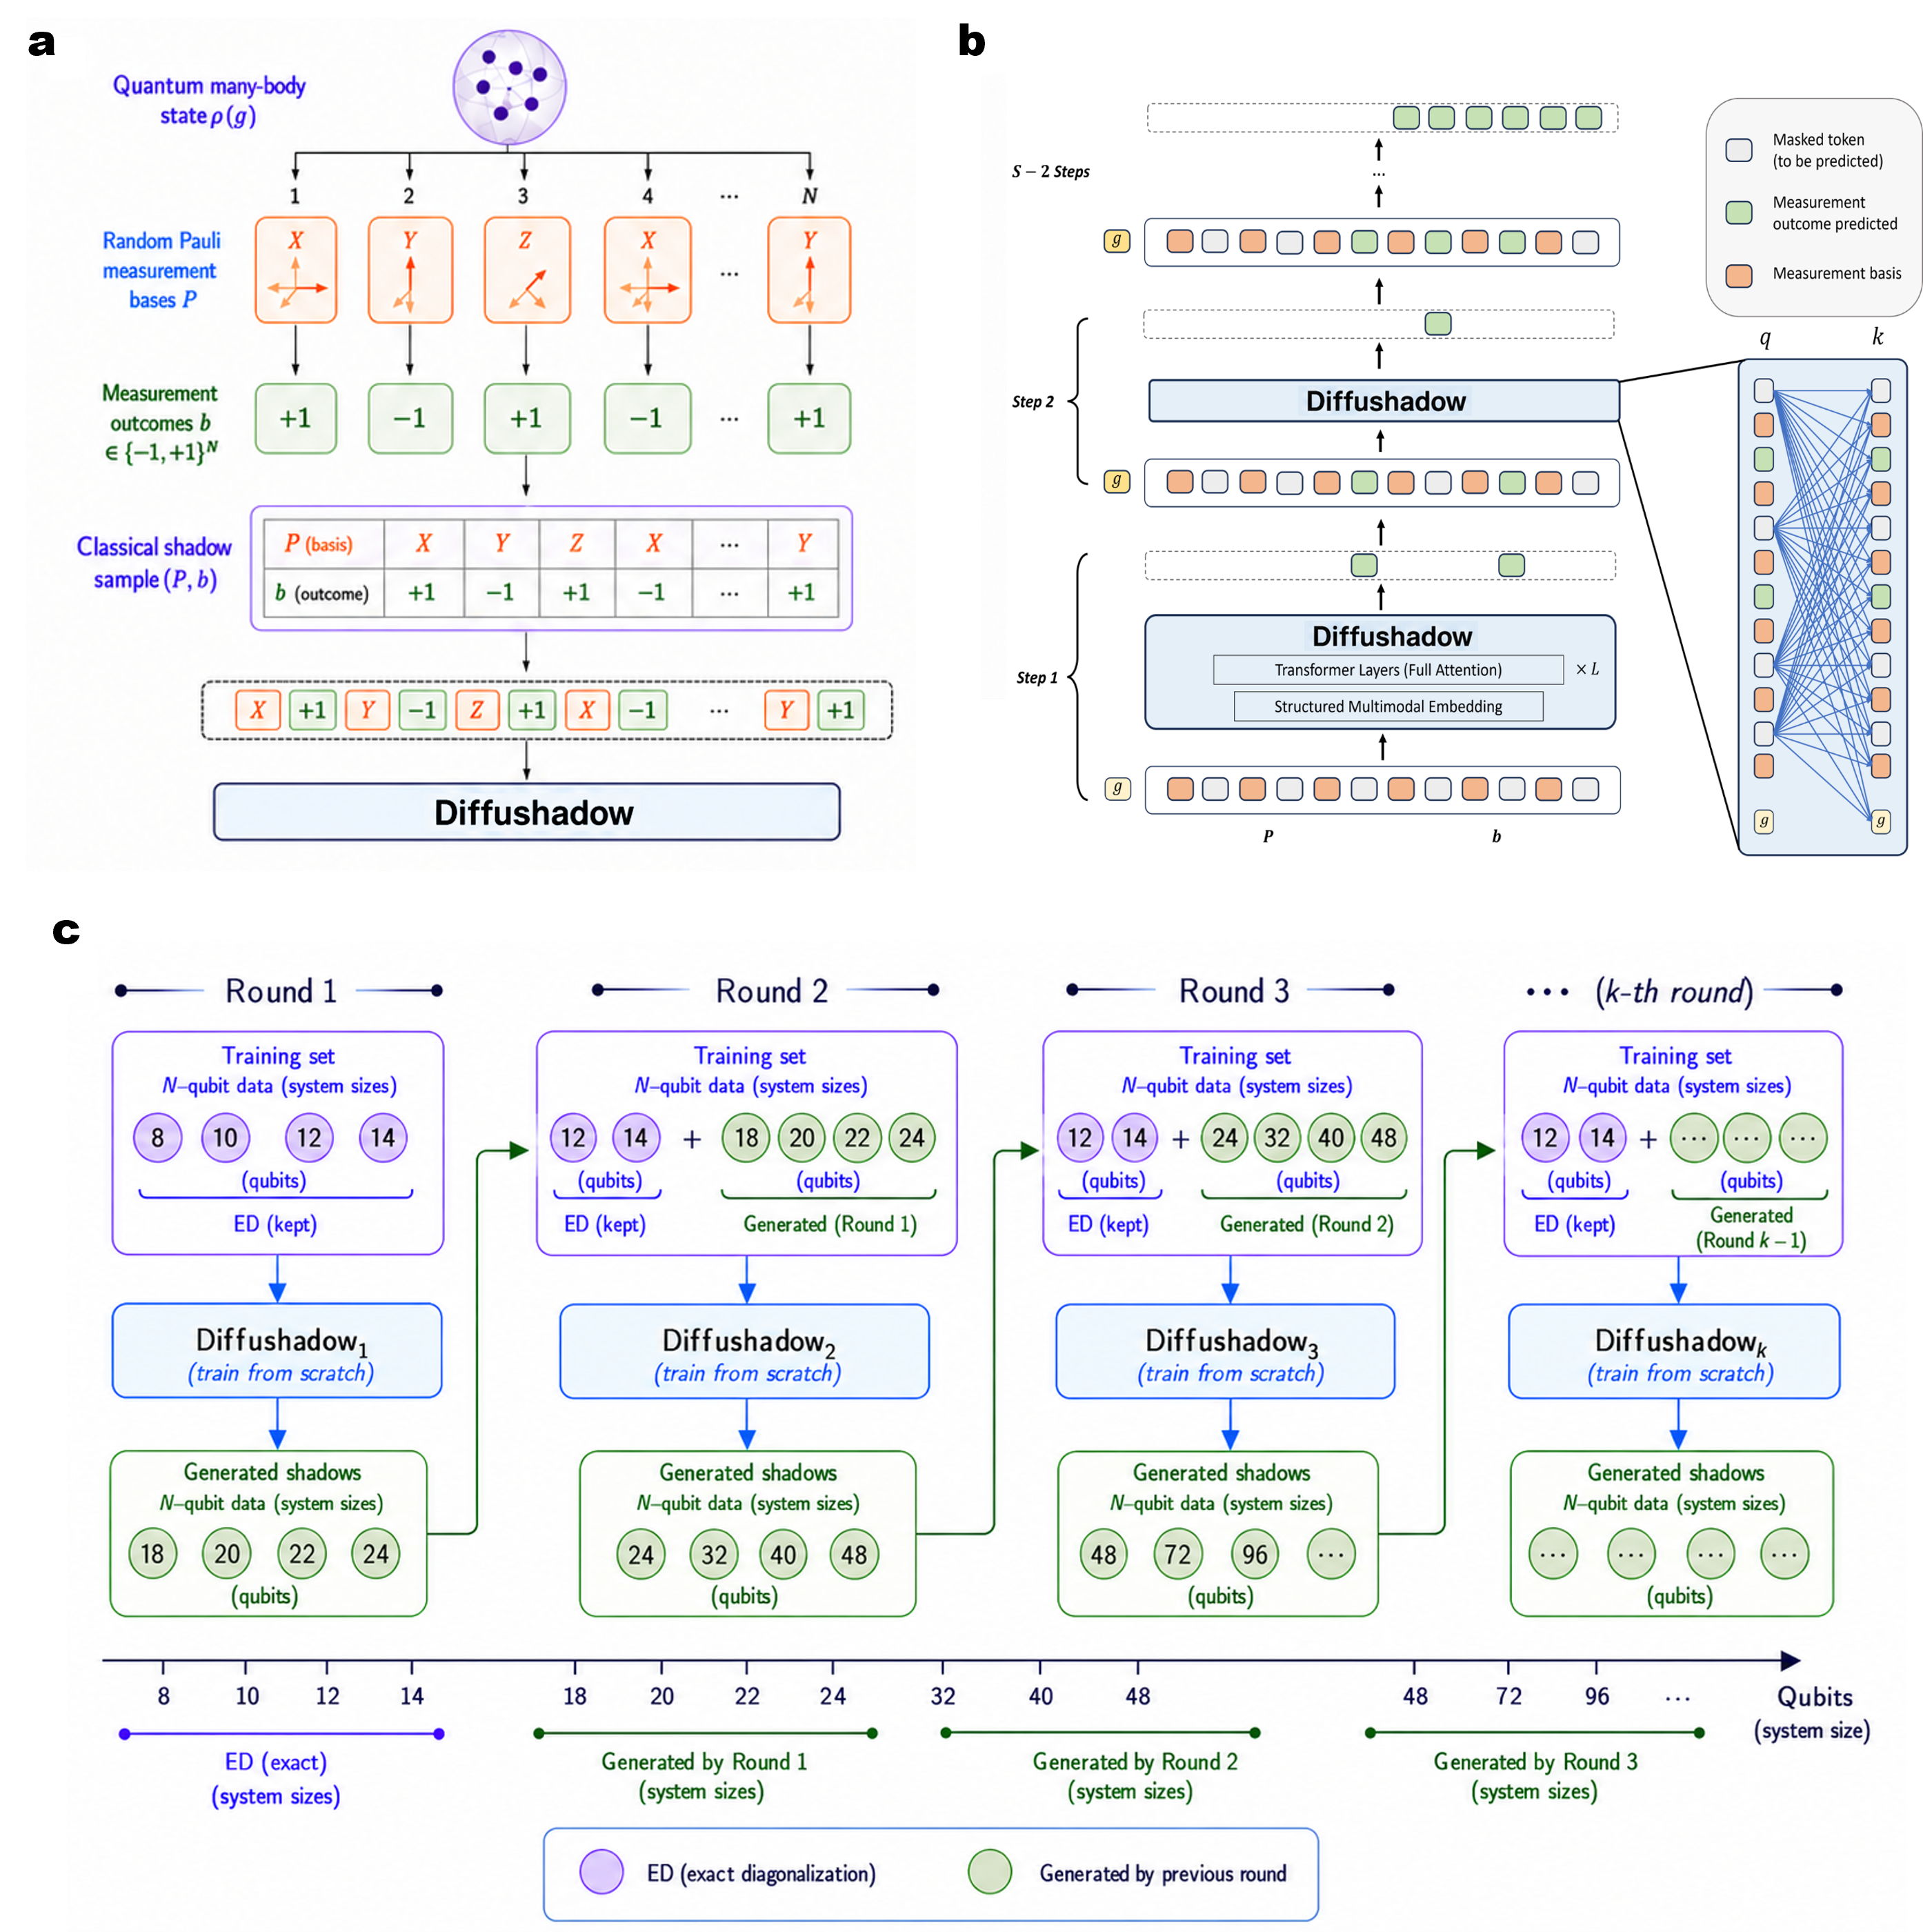
\includegraphics[width=0.98\textwidth]{fig/Figure1_all6.2.png}
\caption{Overview of the Diffushadow framework for cross-scale quantum measurement generation.
\textbf{a} Classical-shadow representation of a quantum many-body state. Each qubit is measured in a randomly selected Pauli basis, and the corresponding measurement outcomes are recorded. The basis sequence $P$ and outcome sequence $b$ together form a classical-shadow snapshot, which is represented as a discrete token sequence for Diffushadow.
\textbf{b} Diffusion-based generation of quantum measurement snapshots. Starting from a fully masked measurement sequence, Diffushadow iteratively denoises the configuration and predicts masked measurement outcomes. Full attention allows the model to aggregate information from both measurement-basis and measurement-outcome tokens across the entire sequence, enabling collective refinement without imposing an autoregressive ordering.
\textbf{c} Recursive scale extrapolation. Diffushadow is first trained on exact small-system classical-shadow data obtained from exact diagonalization, and is then used to generate shadow data for larger systems beyond the original training sizes. The generated data are incorporated into subsequent training rounds together with the retained exact small-system data, progressively expanding the accessible system size. Purple circles denote exact ED data, green circles denote generated data, and braces group the system sizes according to their data source.
}\label{fig1}
\end{figure}

% Diffushadow learns these measurement distributions through masked discrete denoising with full self-attention. Given the physical control parameter, measurement bases and currently available outcomes, the model predicts the outcomes at masked sites without imposing a fixed causal generation order (Fig.~\ref{fig1}b). Full attention therefore allows masked positions to use measurement information distributed throughout the configuration. A causal-mask control confirms this distinction: fixing the outcome of one qubit primarily affects later sequence positions under causal attention, whereas full-attention Diffushadow propagates the change to predictions on both sides of the selected site (Extended Data Fig.~\ref{fig:kl_divergence_attention}).

% Together with full-attention, generation proceeds by iterative unmasking. Starting from a fully or partially masked outcome configuration, Diffushadow predicts the remaining masked sites, reveals selected outcomes according to the decoding rule and then recomputes the predictions using the updated context. Repeating this process produces a complete measurement record with an adaptive rather than predetermined generation order. Iterative decoding substantially reduces the errors of the tested TFI observables relative to one-shot prediction of all outcomes (Extended Data Table~\ref{tab:mse_table}).


% The same denoising formulation supports both unconditional generation and conditional reconstruction. For complete-record generation, all outcomes are initially masked; for reconstruction, observed outcomes remain fixed while only missing sites are denoised. Positional representations encode the spatial organization of the system, allowing the framework to operate across different system sizes and lattice geometries. To extend generation beyond a single size-transfer step, we further introduce recursive scale extrapolation (Fig.~\ref{fig1}c), in which generated measurements at larger sizes are incorporated into subsequent training rounds. We next examine whether these properties enable measurement generation and physical inference beyond the system sizes represented in training.








Diffushadow learns this distribution through masked discrete denoising with full self-attention. Unlike causal attention, full attention allows Diffushadow to predict masked outcomes using information from both preceding and subsequent sites, conditioned on the Hamiltonian parameter, measurement bases and available outcomes (Fig.~\ref{fig1}b). This distinction is illustrated by a causal-mask control in which fixing the measurement outcome of one qubit primarily affects predictions at later sequence positions under causal attention, whereas full-attention Diffushadow propagates the change to predictions on both sides of the selected site (Extended Data Fig.~\ref{fig:kl_divergence_attention}).


Measurement generation proceeds through iterative unmasking. Starting from a fully masked outcome sequence, the model predicts the conditional outcome distributions at all remaining masked sites. At each iteration, the site with the highest predictive confidence is selected, its outcome is sampled and fixed, and the remaining predictions are recomputed using the updated measurement context. The resulting generation order adapts to the model's evolving predictions rather than following a predetermined sequence. Compared with one-shot prediction of all outcomes, iterative decoding substantially reduces errors in the tested TFI observables (Extended Data Table~\ref{tab:mse_table}).

To support cross-scale generation, Diffushadow combines mixed-size training with spatial positional encodings for site positions and two-dimensional lattice coordinates, allowing application to unseen sizes without architectural changes. For further scale extension, recursive scale extrapolation incorporates generated larger-system measurements into successive training rounds alongside retained exact small-system data (Fig.~\ref{fig1}c). 
The same denoising formulation reconstructs incomplete records by keeping observed outcomes fixed while iteratively filling missing positions.







% \section{Results}\label{sec2}
% \subsection{Diffushadow}

% Diffushadow is a discrete diffusion framework for cross-scale generation of quantum measurement records. Figure~\ref{fig1} summarizes its three main components. First, classical-shadow snapshots~\cite{huang2020predicting} provide a site-resolved representation of randomized quantum measurements from which multiple physical observables can be estimated. Second, Diffushadow models these records through full-attention iterative denoising, predicting masked measurement outcomes using information available throughout the configuration without imposing a fixed causal generation order. The site-wise representation and positional encoding allow the same generative formulation to operate on measurement records of different system sizes. To extend generation beyond a single size-extrapolation step, we further develop a recursive scale-extrapolation procedure in which measurements generated for larger systems are incorporated into successive training rounds, progressively expanding the range of system sizes available for physical inference.





% \subsubsection{Classical shadow representation}
% To efficiently represent quantum many-body systems, we adopt classical shadow tomography \cite{huang2020predicting, aaronson2018shadow} as the measurement representation of Diffushadow. Classical shadows provide a compact and experimentally accessible representation of quantum states by storing randomized measurement outcomes instead of the exponentially large density matrix. As illustrated in Fig. \ref{fig1}a, in this framework, each qubit is measured in a randomly selected Pauli basis, and the corresponding measurement outcomes collectively form a classical shadow snapshot of the underlying quantum state. By repeatedly performing randomized measurements, classical shadows enable efficient estimation of a wide range of physical observables \cite{huang2021efficient}, including local correlations and many-body properties, from a limited number of measurements. Importantly, classical shadows naturally preserve physically relevant correlation structures while avoiding the exponential complexity associated with wavefunction-based representations. These properties make classical shadows particularly suitable for scalable generative modeling and finite-size scaling analysis toward the thermodynamic limit. 
% For Diffushadow, each measurement basis and measurement outcome in a single measurement snapshot is modeled as a token, so a single measurement snapshot constitutes a token sequence. This formulation transforms quantum measurement modeling into a discrete generative learning problem, enabling the diffusion model to directly learn the underlying distribution of quantum measurements from experimentally accessible data. 

% \subsubsection{Classical-shadow measurement representation}

% To efficiently represent quantum many-body measurements, we adopt classical shadows~\cite{huang2020predicting,aaronson2018shadow} as the measurement representation of Diffushadow. Classical shadows encode quantum-state information through randomized measurement records without explicitly representing the full density matrix. As illustrated in Fig.~\ref{fig1}a, each qubit is measured in a randomly selected Pauli basis, and the corresponding basis choices and measurement outcomes together form a classical-shadow snapshot. Repeated randomized measurements allow multiple physical observables, including spin correlations and other many-body quantities, to be estimated from the resulting ensemble of snapshots~\cite{huang2021efficient}.

% For Diffushadow, each measurement basis and measurement outcome in a snapshot is represented as a discrete token, producing a site-resolved token sequence whose length grows with system size while retaining a common token vocabulary. This representation converts quantum measurement modeling into a discrete generative learning problem and allows measurement records from different system sizes to be handled within the same model formulation. The diffusion model is then trained to learn the distribution of measurement outcomes conditioned on the measurement bases and the corresponding physical control parameter.

% Classical-shadow measurements have also recently been combined with unsupervised learning to distinguish ordered phases of the ANNNI
% chain~\cite{morais2026distinguishing}. That setting uses shadow-estimated
% correlation features for phase identification. Diffushadow instead
% models the randomized measurement distribution itself and evaluates
% whether the learned distribution can be transferred to larger unseen
% system sizes and used for finite-size extrapolation. 



% \subsubsection{Diffusion generative modeling}

% % Diffushadow models scalable quantum measurement distributions through a diffusion-based generative paradigm designed to capture global and non-local quantum correlations. To model quantum measurement distributions, Diffushadow employs a full-attention mechanism rather than the causal attention commonly used in autoregressive architectures like GPT. Unlike causal attention, which restricts each prediction to depend only on preceding positions in the sequence, full attention enables bidirectional interactions across the entire quantum measurement configuration as schematically illustrated in the right panel of Fig. \ref{fig1}b. The choice of full attention over causal attention is not merely an architectural preference but an alignment with the physical principles governing quantum many-body systems. Quantum systems can exhibit non-local correlations arising from entanglement, and measurement outcomes are not naturally organized as a one-directional causal sequence. 
% % % Causal attention, with its unidirectional mask, fails to capture correlations with subsequent qubits, artificially breaking the inherent symmetry of quantum entanglement. 
% % Full attention enables bidirectional information flow, allowing it to model the global, non-local correlations present in quantum many-body systems. 
% % To further examine the effect of this architectural choice, we performed a causal-mask control experiment. We fixed the measurement outcome of one selected qubit and measured the Kullback-Leibler (KL) divergence between the predicted distributions of the remaining qubits before and after fixation. As shown in Extended Data Fig.~\ref{fig:kl_divergence_attention}, the causal-attention variant mainly propagates this perturbation to later sequence positions, whereas full-attention Diffushadow allows the perturbation to influence qubits on both sides, consistent with bidirectional information flow.

% Diffushadow models quantum measurement records through a masked discrete-denoising process with full self-attention. Unlike autoregressive models, which factorize the measurement sequence according to a fixed causal order, Diffushadow allows each masked outcome to incorporate information from the control parameter, measurement bases, and all currently available outcomes throughout the configuration. As illustrated in Fig.~\ref{fig1}b, full attention therefore provides bidirectional information flow across the measurement record without imposing a predetermined generation direction. To verify this conditioning structure, we perform a causal-mask control experiment in which the outcome of one selected qubit is fixed and the resulting changes in the predicted distributions of the remaining qubits are quantified by the Kullback--Leibler divergence. Extended Data Fig.~\ref{fig:kl_divergence_attention} shows that the causal-attention variant mainly propagates this perturbation to later sequence positions, whereas full-attention Diffushadow allows it to influence predictions on both sides of the selected site.

% Generation proceeds iteratively from a partially or fully masked outcome sequence. At each denoising step, Diffushadow predicts outcome distributions for the remaining masked sites using the current measurement context. Selected sites are then revealed according to the decoding rule, and the predictions for the remaining masked positions are recomputed using the updated context. Repeating this procedure progressively converts the masked sequence into a complete measurement record, with the generation order determined adaptively rather than fixed in advance. Extended Data Table~\ref{tab:mse_table} compares iterative decoding with one-shot generation of all measurement outcomes and shows that iterative denoising yields substantially lower errors for the tested TFI observables.

% The combination of full attention and iterative denoising provides a common mechanism for both complete-record generation and conditional completion. For complete-record generation, all measurement outcomes are initially masked and progressively revealed. For conditional reconstruction, observed outcomes remain fixed while only the missing positions are denoised. This common formulation allows the same trained model to operate under different patterns of available measurement information without introducing a separate reconstruction objective.


% While full attention provides a mechanism for capturing global correlations within a quantum measurement configuration, Diffushadow further leverages this capability through an iterative denoising process, as illustrated in the left panel of Fig. \ref{fig1}b. Unlike autoregressive architectures that generate measurement outcomes sequentially through causal attention, Diffushadow refines all qubits collectively and generates measurement outcomes in no predetermined order during the denoising process. 
% % This generative paradigm of Diffushadow enables bidirectional interactions across the entire measurement configuration and allows the model to capture global correlations without imposing an artificial sequential dependency on the generated measurements. 
% This design is better aligned with the nature of quantum many-body systems, where measurement outcomes collectively reflect the same underlying quantum state rather than being generated through an intrinsic causal chain. Extended Data Table \ref{tab:mse_table} reports numerical experiments comparing iterative-generation Diffushadow with one-shot generation of all measurement outcomes. The results confirm that iterative generation achieves superior accuracy.
% With full attention and iterative denoising, Diffushadow provides an inductive bias for modeling global dependencies in quantum measurement configurations, demonstrating strong potential for effective modeling. Extended Data Table~\ref{tab:mse_table} further compares Diffushadow with the autoregressive ShadowGPT baseline \cite{yao2024shadowgpt} in the TFI model, supporting the effectiveness of full-attention iterative denoising for modeling globally correlated quantum measurement configurations.

% In addition to full attention, Diffushadow generates quantum measurements through iterative denoising. Unlike autoregressive architectures that generate measurement outcomes sequentially in a predetermined order, Diffushadow collectively refines all qubits during the denoising process. This generative paradigm allows all measurement outcomes to emerge simultaneously from the same underlying quantum state rather than through an artificial sequential dependency. By enabling collective refinement across the entire system, Diffushadow more effectively captures global and long-range quantum correlations in scalable quantum many-body systems.



\begin{figure}[htbp!]
\centering
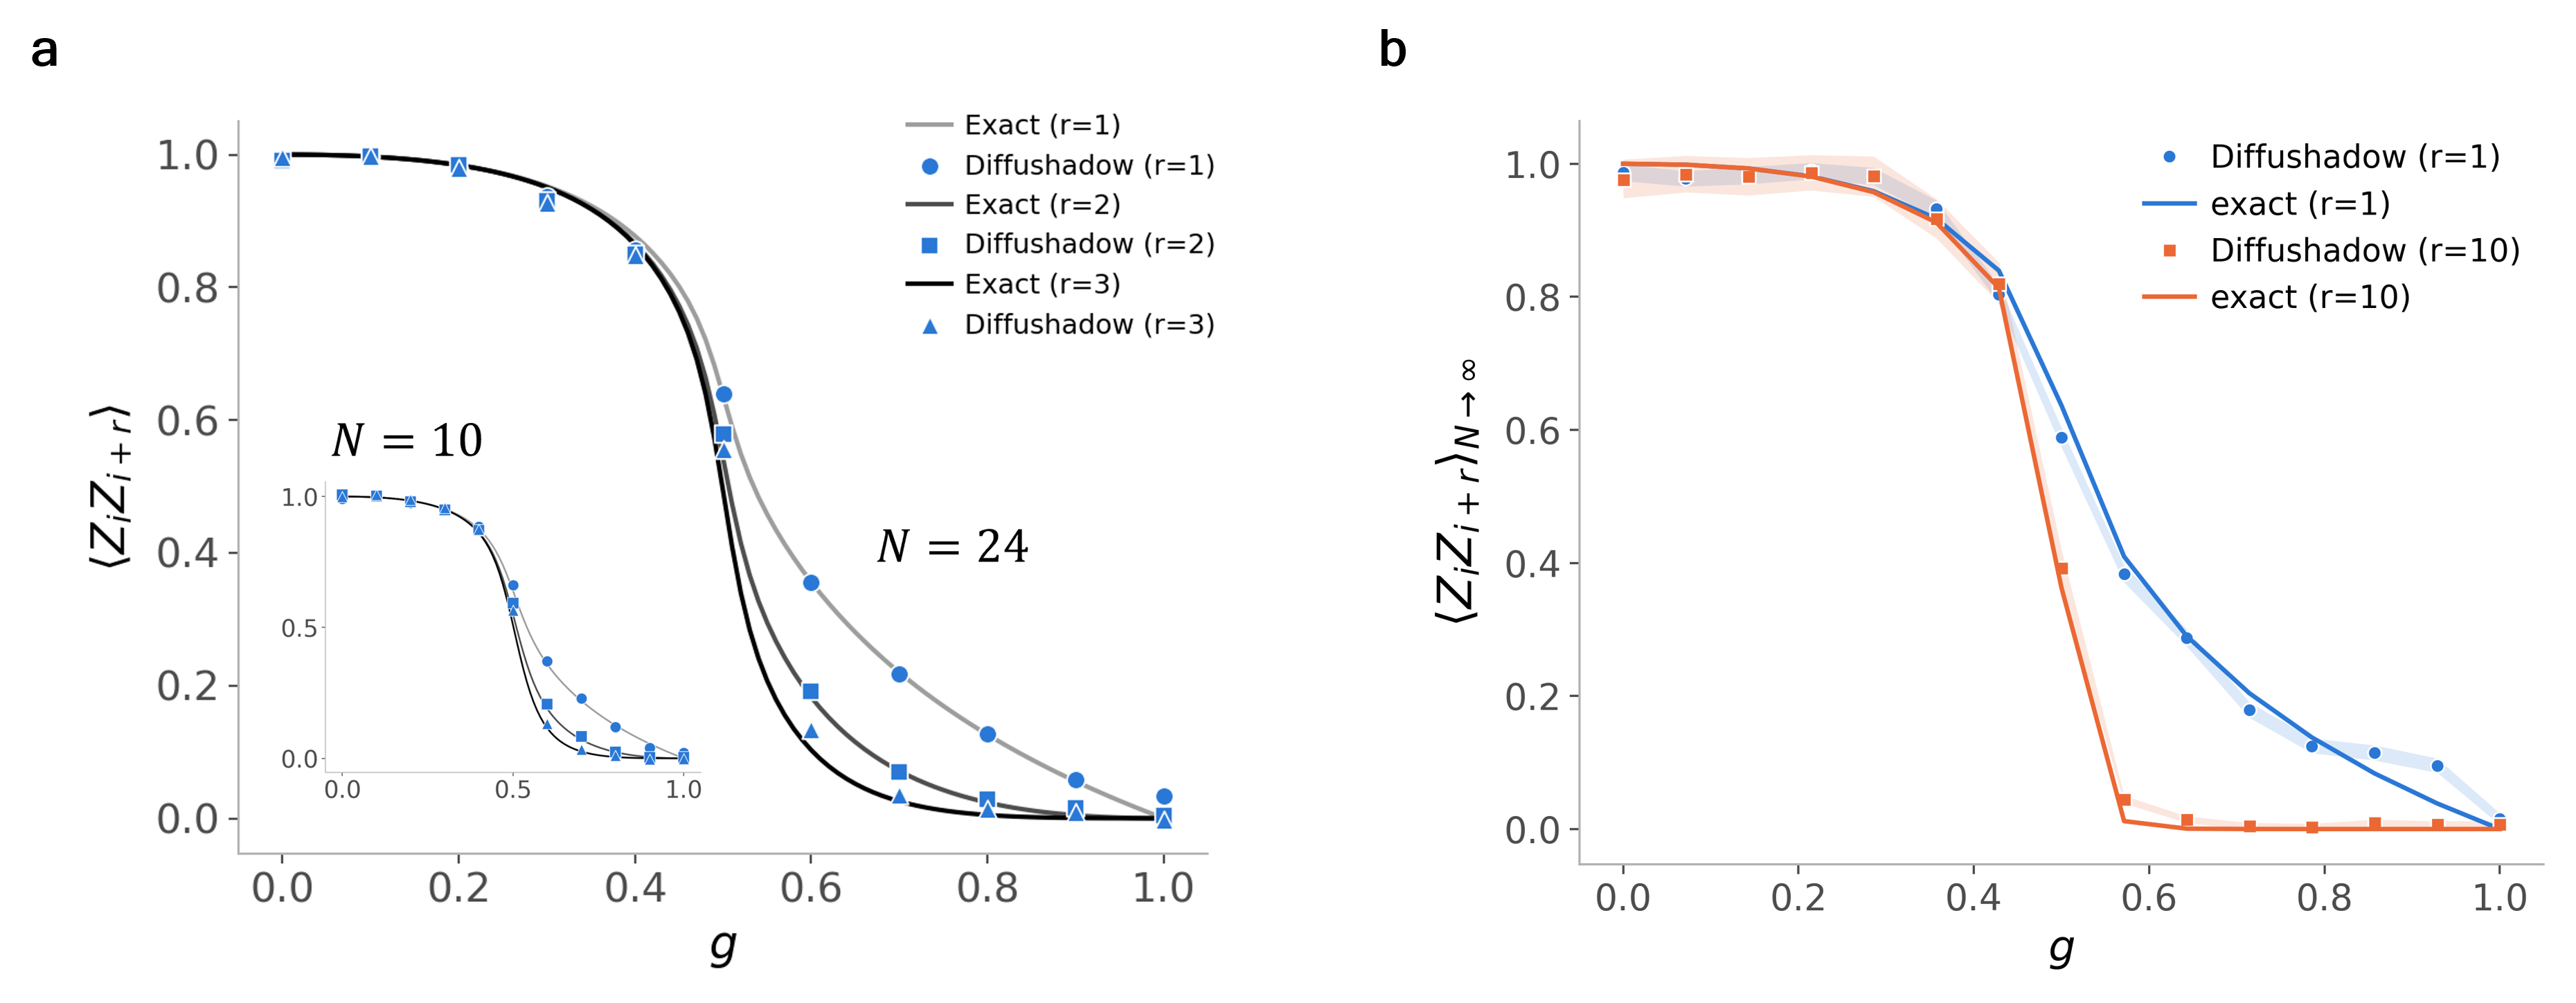
\includegraphics[width=0.98\textwidth]{fig/Figure2_tfi.png}
\caption{\textbf{Cross-scale generation and thermodynamic-limit inference in the transverse-field Ising model.}
\textbf{a}, Longitudinal spin correlations $(\langle Z_i Z_{i+r}\rangle)$ for $r=1,2,3$ at the unseen system size $N=24$, with the training size $N=10$ shown in the inset. Solid curves show exact diagonalization results, and markers show estimates from Diffushadow-generated classical-shadow measurements. 
\textbf{b}, Thermodynamic-limit correlations for $r=1$ and $r=10$, obtained by linear extrapolation in $1/N$ of observables estimated from recursively generated measurements. Solid curves show exact thermodynamic-limit results, and markers show Diffushadow estimates. Shaded regions indicate pointwise 95\% bootstrap confidence intervals.}
\label{fig2}
\end{figure}


% \subsubsection{Validation across representative spin-chain Hamiltonians}

% We conducted experiments on Diffushadow to verify whether it can effectively model the measurement data of quantum many-body systems. We begin by validating Diffushadow on finite-size instances of representative one-dimensional quantum spin-chain Hamiltonians, ranging from the transverse-field Ising model \cite{pfeuty1970one} to frustrated and competing-interaction models such as the $J_1$-$J_2$ chain \cite{majumdar1969next, majumdar1969next2} and the axial next-nearest-neighbor Ising (ANNNI) model \cite{selke1988annni}. These models cover both a canonical quantum phase-transition benchmark and spin-chain systems with competing interactions, providing a testbed for assessing whether Diffushadow can model quantum measurement distributions beyond a single Hamiltonian. For each Hamiltonian, Diffushadow is trained on small-system classical-shadow measurements and used to generate measurement snapshots of the same size. Physical observables estimated from the generated measurements are then compared with exact results. Figure \ref{fig2} a-c present the ground state property estimated by the data generated by Diffushadow for the transverse-field Ising model, the $J_1$-$J_2$ model, and the ANNNI model, respectively. We focus on the correlation function $<Z_iZ_{i+r}>, r=1,...,5$ of order parameters. In the figure, solid lines correspond to exact diagonalization results, and blue scattered points indicate predictions made by Diffushadow. It is evident that Diffushadow's estimates closely align with the exact solutions across the parameter $g$. This suggests that our model attains a high degree of predictive accuracy. On the other hand, considering our model is trained on a few different sparse values of $g$, the results show that our model exhibits promising generalization capabilities. This is significant for the efficient generation of a large amount of shadow data with diverse $g$ values. 
% These results demonstrate that Diffushadow generates measurements that reproduce key ground-state observables at trained system sizes, providing a foundation for accurate physical-property estimation.




% We next examine whether the learned measurement structures can transfer to larger systems not observed during training. For this purpose, Diffushadow is trained on mixed-size measurement data from smaller systems and then used to generate measurements for larger target systems. Figures~\ref{fig2}d--f and \ref{fig2}g--i present cross-size generation results for 20- and 24-qubit systems, respectively. Within each row, the three panels correspond to the transverse-field Ising model, the $J_1$--$J_2$ model, and the ANNNI model. The generated-measurement estimates remain close to the exact results across these larger system sizes, indicating that Diffushadow can generalize beyond the system sizes used during training in these spin-chain settings. This behavior is consistent with the model learning measurement structures that are transferable across finite-size instances, rather than relying solely on size-specific training patterns.



\subsection{Cross-scale generation and thermodynamic-limit inference in the TFI model}

% We have demonstrated that Diffushadow is capable of learning transferable quantum structures and generalizing to larger quantum many-body systems. However, direct zero-shot extrapolation alone remains insufficient for approaching the thermodynamic limit. To further extend the accessible system size of Diffushadow, we introduce a recursive scale extrapolation procedure, which is a progressive scale-expansion framework for quantum measurement generation. This process begins with Diffushadow being trained on a mixed dataset of accurately generated measurement data from several small-scale quantum many-body systems. Then, we employ the trained Diffushadow to produce measurement data for larger-scale quantum many-body systems, thereby completing the first round of iteration. In the second round of training, Diffushadow is trained from scratch using the data generated in the first round along with a portion of the accurate data used in the first round. Similar to the first round, in the second round Diffushadow again generates quantum many-body data of a larger scale than the data it was trained on. All subsequent rounds proceed in the same manner. It is worth noting that the only exact data used throughout the entire process are the small-scale quantum many-body data employed in the first round of training. This is largely due to the fact that data from smaller quantum systems are both easily accessible and highly accurate.

% Having introduced the iterative denoising framework of Diffushadow, we next evaluate whether this generative model can support quantum measurement inference beyond the system sizes used for training. We first focus on the transverse-field Ising model, which provides a controlled benchmark with a well-characterized transition between ferromagnetic and paramagnetic regimes. In this section, we use longitudinal spin correlations \(\langle Z_i Z_{i+r}\rangle\) as representative physical observables for assessing both finite-size generation and scale transfer. As summarized in Fig.~\ref{fig2}a--d, we first evaluate measurement generation at system sizes represented in training, then test direct generation at larger unseen sizes, and finally apply recursive scale extrapolation to obtain measurement ensembles over an expanded range of system sizes for thermodynamic-limit inference.

To assess cross-scale measurement generation, we consider the one-dimensional transverse-field Ising (TFI) model with periodic boundary conditions, described by $H=-(1-g)\sum_i Z_iZ_{i+1}-g\sum_i X_i$, where $g$ controls the competition between ferromagnetic interactions and transverse-field quantum fluctuations. In the thermodynamic limit, the critical point $g_c=0.5$ separates ferromagnetic and paramagnetic phases. Longitudinal spin correlations $\langle Z_iZ_{i+r}\rangle$ characterize the spatial correlations of the ground state, remaining extended in the ordered regime and decaying with separation in the paramagnetic regime. Their dependence on both $g$ and $r$ also provides a probe of the measurement statistics generated by Diffushadow.

% Having introduced the generative framework of Diffushadow, we first evaluate whether measurement statistics learned from small systems can transfer to larger unseen system sizes. We use the transverse-field Ising (TFI) model as a controlled benchmark, owing to its well-characterized ferromagnetic-to-paramagnetic transition and finite-size behavior. Longitudinal spin correlations, \(\langle Z_i Z_{i+r}\rangle\), serve as representative observables for assessing both finite-size generation and scale transfer. As summarized in Fig.~\ref{fig2}a--d, we first evaluate measurement generation at system sizes represented in training, then test direct generation at larger unseen sizes, and finally apply recursive scale extrapolation to obtain measurement ensembles over an expanded range of system sizes for thermodynamic-limit inference.

\subsubsection{Cross-scale measurement generation in the TFI model}

% Before using generated measurements for thermodynamic-limit inference, we first assess whether Diffushadow can reproduce finite-size transverse-field Ising observables both within and beyond the training system sizes.

% As a same-size benchmark, Diffushadow is first trained and evaluated on 10-qubit TFI systems. 
% % This setting provides a direct test of whether the learned generative model can reproduce physical observables from classical-shadow measurement samples at system sizes included in training. 
% As shown in Fig.~\ref{fig2}a, spin-spin correlation functions \(\langle Z_i Z_{i+r}\rangle\) estimated from Diffushadow-generated measurements closely follow the exact diagonalization results across the scanned transverse-field parameter \(g\). The agreement demonstrates that Diffushadow can generate measurement samples that preserve the longitudinal correlation structure of the TFI ground state at training system size. The corresponding mean squared errors between Diffushadow estimates and exact results are reported in Extended Data Table~\ref{tab:mse_table}. The same table compares Diffushadow with the autoregressive ShadowGPT baseline~\cite{yao2024shadowgpt}, with Diffushadow yielding lower errors.

% Beyond faithfully modeling quantum measurements within the training regime, an important question is whether Diffushadow can generalize the learned quantum measurement structures to larger quantum systems that are inaccessible during training. To investigate this question, Diffushadow is trained on mixed-size measurement data from smaller systems and then used to generate measurements for larger target systems that were never observed during training. 
% By exposing the model to measurements from multiple scales during training, Diffushadow is encouraged to learn quantum structures that are shared across system sizes rather than size-specific patterns tied to a particular finite system.
% Fig. \ref{fig2}b presents the cross-scale generation results for 24-qubit systems, which are larger than the systems used during training. In this figure, the generated-measurement estimates remain close to the exact results, indicating that Diffushadow can generalize to larger unseen system sizes in these spin-chain settings. This suggests that Diffushadow does not merely reproduce size-specific training measurement patterns, but instead learns quantum structures that remain transferable across system scales. These learned structures enable the model to extrapolate beyond the original training regime and generate physically meaningful quantum measurements for larger many-body systems.
% Beyond faithfully modeling quantum measurements within the training regime, an important question is whether the learned measurement statistics remain transferable to larger system sizes that are not represented during training. To investigate this question, Diffushadow is trained on mixed-size measurement data from smaller systems and then used to generate measurements for larger target systems that were never observed during training. By exposing the model to measurements from multiple system sizes, mixed-size training encourages it to capture measurement statistics that persist across scales rather than patterns specific to a particular finite system.
% Figure~\ref{fig2}b presents the cross-scale generation results for 24-qubit systems, compared with a largest training size of $N=14$. The generated-measurement estimates remain close to the exact results across the tested correlations, demonstrating direct cross-scale transfer of the learned measurement statistics in these spin-chain settings. These results show that Diffushadow does not merely reproduce size-specific training distributions: statistics learned from smaller systems remain predictive at larger unseen sizes, providing the basis for the recursive scale extrapolation developed below.


We first evaluate measurement generation at the training size $N=10$. As shown in the inset of Fig.~\ref{fig2}a, correlations at $r=1,2,3$ estimated from Diffushadow-generated classical shadows closely follow exact diagonalization (ED) results across the scanned values of $g$, including the rapid suppression of longitudinal correlations near the critical region. Comparisons of the ground-state energy and selected spin correlations with the autoregressive ShadowGPT baseline~\cite{yao2024shadowgpt} are reported in Extended Data Table~\ref{tab:mse_table}, where Diffushadow achieves lower mean squared errors across the reported observables and coupling values.

% For direct cross-scale generation, Diffushadow is trained on mixed-size measurements from $N=8,10,12,14$ and evaluated on the unseen $N=24$ chain without retraining. Figure~\ref{fig2}a shows that the generated measurements reproduce the field and distance dependence of the longitudinal correlations. At weak transverse fields, correlations at all three separations remain close to unity, reflecting ferromagnetic ordering. As $g$ approaches the critical region, the correlations decrease rapidly and become increasingly dependent on separation. Beyond the transition, longer-range correlations approach zero more rapidly than nearest-neighbour correlations. Diffushadow captures these distinct trends across $r=1,2,3$, although deviations are visible near the critical region and at larger $g$, particularly for the nearest-neighbour correlation. The agreement with ED at $N=24$ establishes direct transfer of the tested correlation statistics beyond the system sizes represented in training.


For direct cross-scale generation, Diffushadow is trained on mixed-size measurements from $N=8,10,12,14$ and evaluated on the unseen $N=24$ chain without retraining. Figure~\ref{fig2}a shows that the generated measurements reproduce both the field dependence and spatial separation of the longitudinal spin correlations. At weak transverse fields, Diffushadow recovers the near-unity correlations at all three separations, characteristic of the ferromagnetic regime. Near the critical region, the generated estimates follow the rapid suppression of correlations and the increasing differences between $r=1,2,3$. In the paramagnetic regime, Diffushadow distinguishes the more persistent nearest-neighbour correlations from the faster decay of correlations at larger separations, rather than reproducing only their overall decrease with $g$. Deviations from ED remain visible near the critical region and at selected larger field strengths, particularly for the nearest-neighbour correlation. The simultaneous recovery of field-dependent and distance-dependent correlation behaviour at $N=24$ demonstrates that the learned measurement statistics remain transferable beyond the system sizes represented in training.



% \subsubsection{Thermodynamic-limit inference from recursively generated measurements}

% Direct zero-shot extrapolation does not by itself provide the range of system sizes needed for thermodynamic-limit inference. We therefore introduce recursive scale extrapolation (Fig.~\ref{fig1}c), in which generated larger-system measurements are incorporated into the training data for the next round. Starting from exact measurements for systems with at most $N=14$ spins, three recursive rounds extend generation to $N=96$. Rather than introducing additional exact large-system information, the procedure iteratively propagates the cross-scale structure learned from smaller systems, while retaining exact small-system measurements as a reference. Supplementary Fig.~5 shows that 24-qubit observables generated by models from different recursive rounds remain largely consistent, indicating limited drift at the tested scale.

% We then use the recursively generated ensembles for finite-size analysis of the TFI spin correlations $\langle Z_i Z_{i+r}\rangle$. Following the finite-size-scaling paradigm, we fit the observables as functions of $1/N$~\cite{privman1990finite,cardy1996scaling}, using the empirical fitting form specified in Methods. The resulting thermodynamic-limit estimates for $r=1$ and $r=10$ are shown in Fig.~\ref{fig2}c,d. The extrapolated Diffushadow estimates reproduce the overall correlation profiles across the ferromagnetic and paramagnetic regimes. Deviations are largest near the critical region and for the longer-range $r=10$ correlation, which also exhibits broader bootstrap confidence intervals.

% Together, these results indicate that recursively generated measurements preserve the systematic finite-size evolution of the TFI correlations and, together with the extrapolation protocol, support thermodynamic-limit inference with explicitly quantified statistical uncertainty.



\subsubsection{Thermodynamic-limit inference from recursively generated measurements}

To extend the system sizes available for finite-size inference, we employ recursive scale extrapolation (Fig.~\ref{fig1}c). Starting from exact measurements for systems with at most $N=14$ spins, each subsequent round trains a newly initialized model on larger-system measurements generated by the preceding model, together with retained exact small-system data. Three recursive rounds extend generation to $N=96$ without introducing additional exact large-system measurements. Observable estimates at $N=24$ remain largely consistent across different recursive rounds (Extended Data Fig.~\ref{fig:stability_analysis}), indicating limited drift at the tested scale.

The recursively generated measurement ensembles provide finite-size estimates of the longitudinal correlations $\langle Z_iZ_{i+r}\rangle$. For each field strength $g$ and separation $r$, we perform an empirical linear extrapolation in inverse system size~\cite{privman1990finite,cardy1996scaling}, using $C_{ZZ,N}(r,g)=C_{ZZ,\infty}(r,g)+a(r,g)/N$. The intercept at $1/N=0$ gives the thermodynamic-limit estimate, which is compared with the exact reference in Fig.~\ref{fig2}b. Pointwise 95\% bootstrap confidence intervals quantify the sampling uncertainty propagated through the finite-size fits.

% Figure~\ref{fig2}b shows the extrapolated correlations at $r=1$ and $r=10$, probing short- and longer-range spin correlations, respectively. In the ferromagnetic regime ($g<0.5$), both correlations remain strong, consistent with the long-range order of the ground state. Near the critical point, the correlations decrease rapidly, with a more pronounced suppression at larger separation. In the paramagnetic regime ($g>0.5$), the $r=10$ correlation approaches zero, whereas the nearest-neighbour correlation remains finite and decreases more gradually with increasing field. Diffushadow reproduces this contrasting distance dependence and the overall field evolution of both observables, with visible deviations near the transition and at some field strengths in the paramagnetic regime.

Figure~\ref{fig2}b compares the thermodynamic-limit correlations inferred from recursively generated Diffushadow measurements with exact TFI results at $r=1$ and $r=10$. The extrapolated estimates closely follow the reference profiles across the scanned transverse fields, reproducing strong correlations at both separations in the ferromagnetic regime and their rapid suppression near the critical region. Importantly, Diffushadow captures the contrasting behaviour of the two correlation distances in the paramagnetic regime. The longer-range $r=10$ correlation rapidly approaches zero, whereas the nearest-neighbour correlation remains appreciable and decreases more gradually with increasing field. This agreement shows that the recursively generated measurement ensembles retain sufficient spatial correlation information to distinguish short- and longer-range behaviour after extrapolation to the thermodynamic limit. Although deviations remain at selected field strengths, particularly for $r=1$ in the paramagnetic regime, Diffushadow reproduces the principal features of both exact thermodynamic-limit correlation profiles.



\begin{figure}[htbp!]
\centering
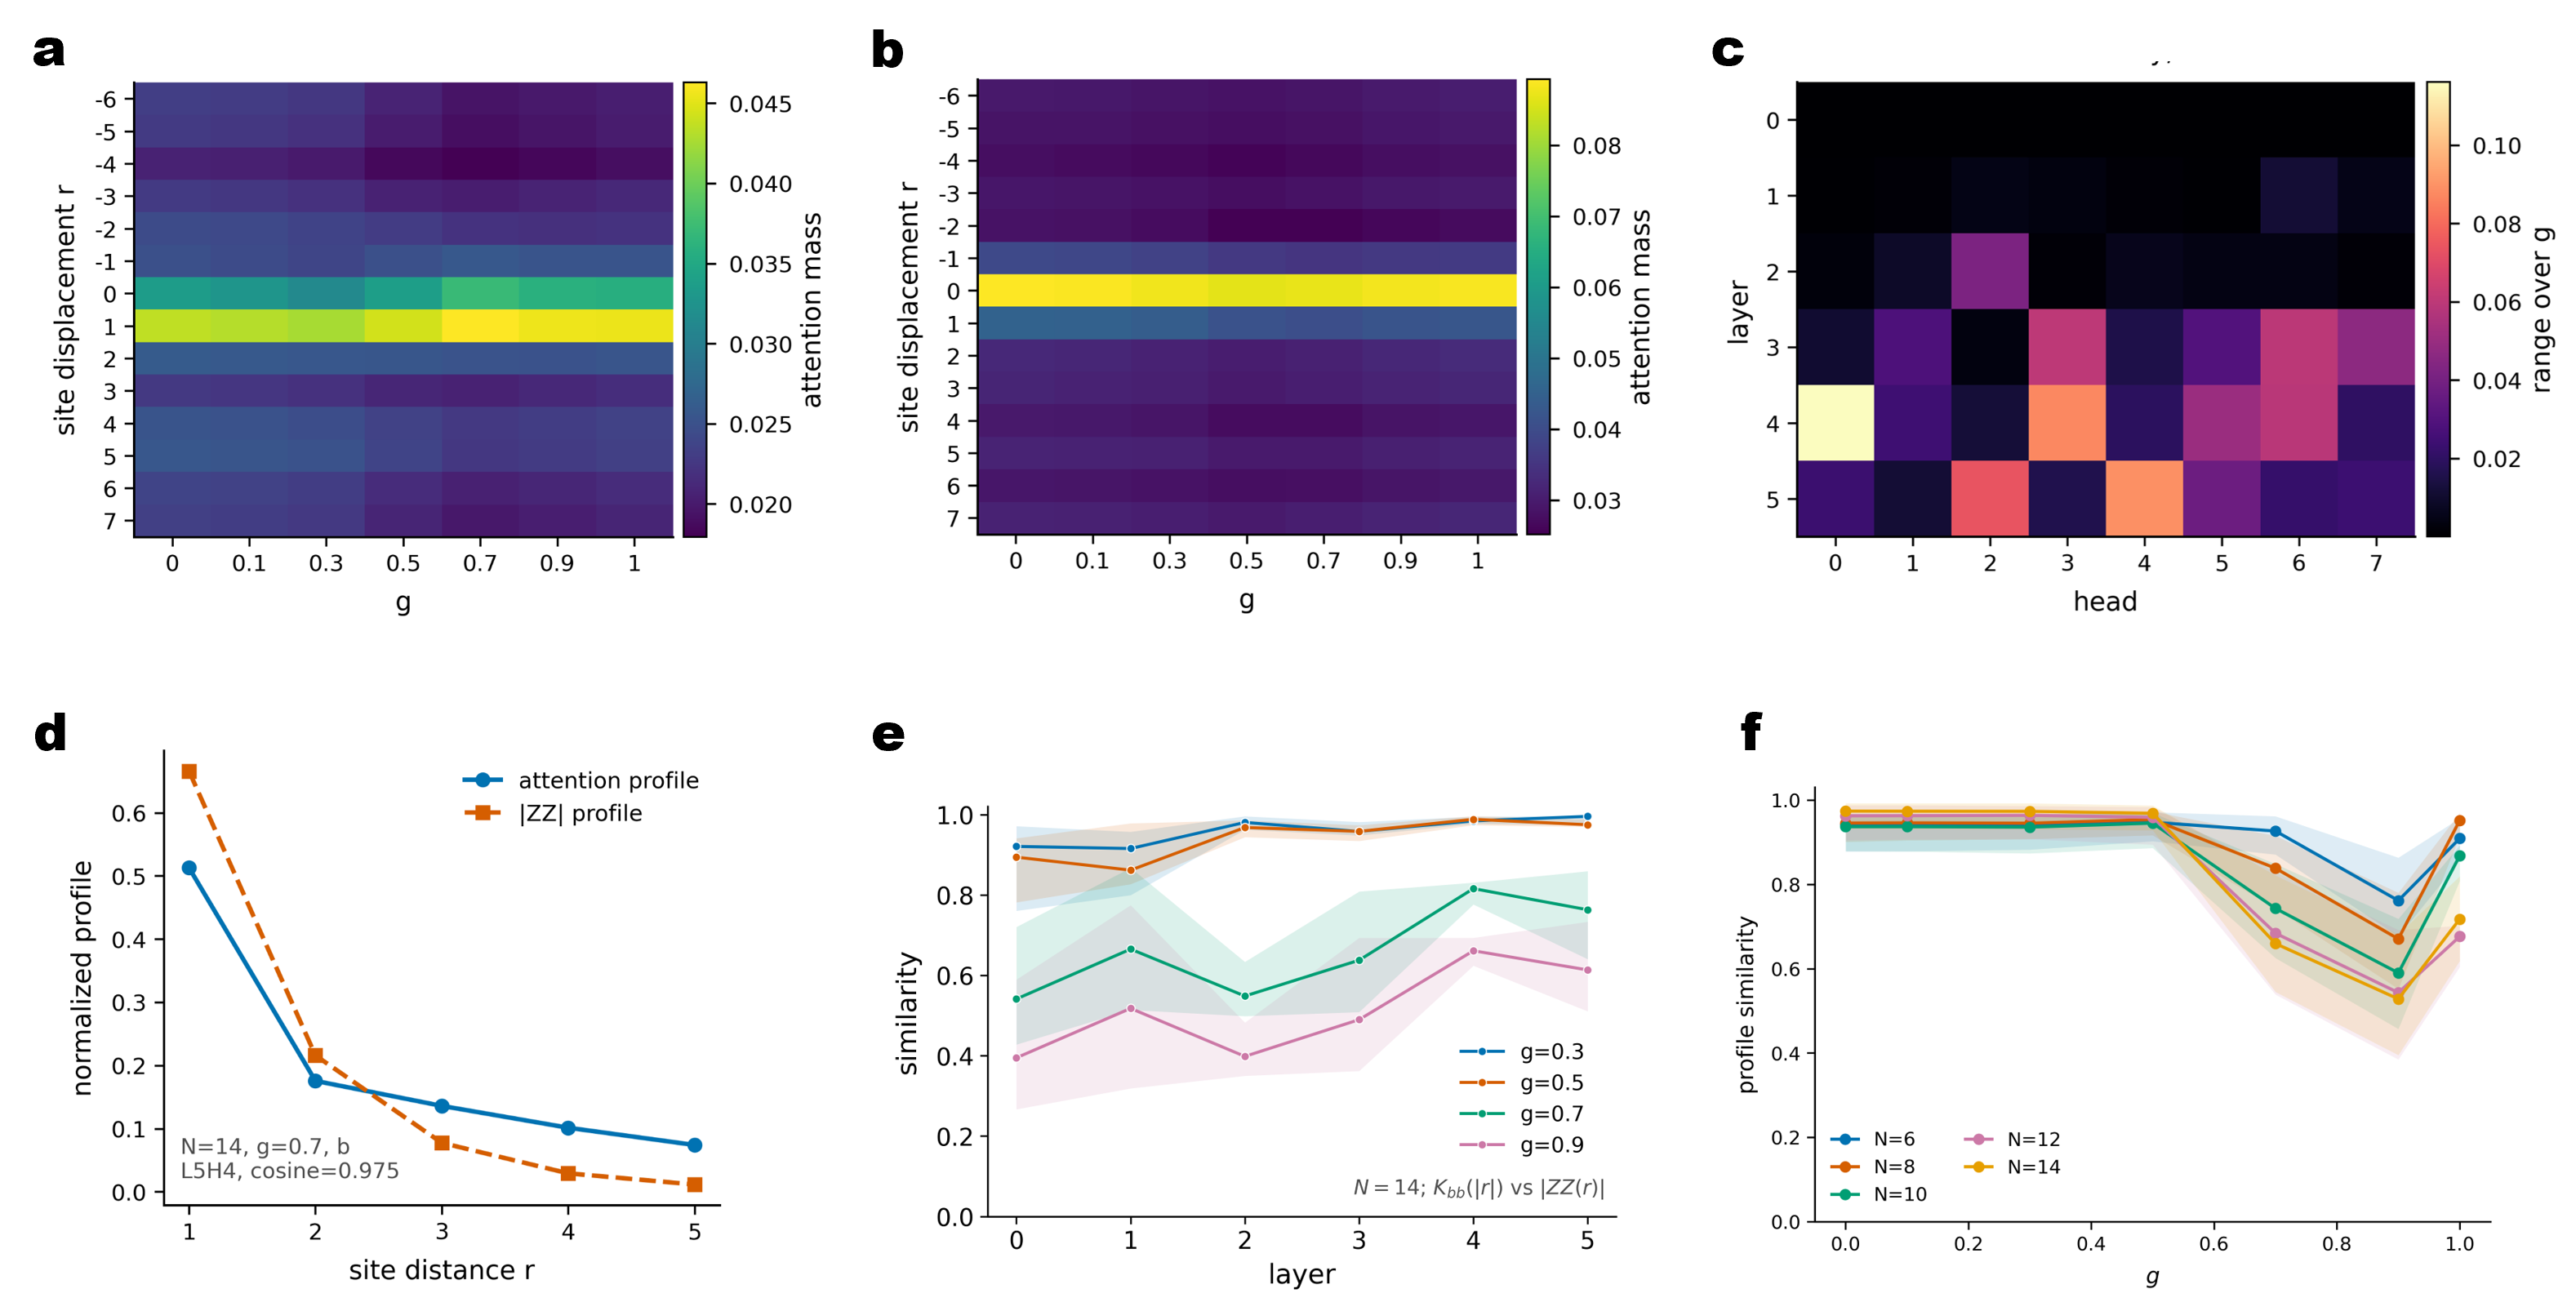
\includegraphics[width=0.98\textwidth]{fig/Figure2_attn_analysis.png}
\caption{
\textbf{Spatial attention patterns and alignment with spin correlations in the transverse-field Ising model.}
Attention is evaluated with all measurement-outcome tokens masked. Panels a--e use $N=14$.
\textbf{a,b,} Attention kernels from masked outcome queries to outcome tokens, $K_{bb}(r,g)$ (a), and measurement-basis tokens, $K_{bP}(r,g)$ (b), as functions of signed periodic site displacement $r$ and transverse-field parameter $g$. Colours indicate attention mass averaged over query sites, measurement-basis configurations, heads and layers.
\textbf{c,} Variation in the attention-weighted mean site distance across $g$ for each layer--head pair. Colour indicates the range $\Delta D^{(\ell,h)}=\max_g D^{(\ell,h)}(g)-\min_g D^{(\ell,h)}(g)$.
\textbf{d,} Absolute-distance attention kernel $K_{bb}(|r|)$ and exact absolute correlation profile $|\langle Z_i Z_{i+r}\rangle|$ for head L5H4 at $g=0.7$, selected for the highest cosine similarity at this setting. Each profile is normalized to unit sum over the displayed distances.
\textbf{e,} Median cosine similarity across heads within each layer between outcome-directed attention kernels and exact absolute $ZZ$ correlation profiles, shown at $g=0.3,0.5,0.7$ and $0.9$.
\textbf{f,} Median cosine similarity across all layer--head pairs as a function of $g$ for $N=6,8,10,12$ and $14$. Shading denotes the interquartile range across heads within each layer in e and across all layer--head pairs in f. Layer and head indices are zero-based.
}
\label{fig3}
\end{figure}


% \subsubsection{Thermodynamic-limit inference from recursively generated measurements}


% We have demonstrated that Diffushadow is capable of learning transferable quantum structures and generalizing to larger quantum many-body systems. However, direct zero-shot extrapolation alone remains insufficient for approaching the thermodynamic limit. To further extend the accessible system size of Diffushadow, we introduce a recursive scale extrapolation procedure, which is a progressive scale-expansion framework for quantum measurement generation, as shown in Fig.~\ref{fig1}c.
% The procedure begins with Diffushadow being trained on a mixed dataset consisting of accurate measurement data from several small-scale quantum many-body systems. The trained model is then used to generate measurement data for larger systems beyond the original training regime. These generated measurements are subsequently incorporated into the training data for the next round, enabling the model to progressively expand its accessible system size. By iteratively repeating this process, Diffushadow progressively transfers the learned quantum measurement structures to increasingly larger quantum many-body systems. In the present implementation, three recursive rounds expand the accessible system size from exact training data with at most $N=14$ spins to generated measurement data for systems as large as $N=96$. The stability of this recursive procedure is further examined in Supplementary Fig. 5, where 24-qubit observables generated by Diffushadow models from different recursive rounds remain largely consistent, suggesting that the recursive training process does not introduce substantial drift at the tested scale.
% % To assess the stability of recursive scale extrapolation, we further compare 24-qubit predictions from Diffushadow models trained in different recursive rounds in the Supplementary Information. The predictions remain largely consistent across rounds, suggesting that incorporating generated measurements into subsequent training stages does not introduce substantial drift or error accumulation in this setting.
% % Instead, the learned quantum structures remain remarkably stable throughout the recursive expansion process, allowing Diffushadow to consistently reproduce physically meaningful quantum measurements at scales beyond the original training regime.
% Throughout the entire recursive extrapolation process, the only exact data required are the small-scale quantum measurements used during the initial training stage. All subsequent generations are derived from the recursively expanded models, allowing the accessible system size to grow far beyond that of the original training data. This reduces the dependence on large-scale exact measurements, which are often prohibitively expensive to obtain from either numerical simulations or quantum experiments.

% As a result, recursive scale extrapolation provides a practical pathway for extending quantum measurement modeling toward system sizes that would otherwise remain inaccessible, thereby enabling thermodynamic-limit inference from a small set of exact measurements together with recursively generated large-scale quantum data.


% Having established the ability of Diffushadow to generate physically consistent quantum measurements at scales far beyond the original training regime, we next seek to infer physical properties in the thermodynamic limit. We focus on the spin-spin correlation function $\langle Z_i Z_{i+r} \rangle$, a fundamental observable for characterizing quantum phases and correlation structures in the transverse-field Ising model.

% The large-scale quantum measurements generated through recursive scale extrapolation provide access to system sizes that would otherwise be inaccessible using the original training data alone. Following the standard finite-size scaling paradigm in many-body physics, observables extracted from the generated measurements are analyzed as functions of the inverse system size $1/N$ \cite{privman1990finite, cardy1996scaling}. 
% % The resulting scaling curves are then extrapolated to the limit $1/N \rightarrow 0$, corresponding to the thermodynamic limit $N \rightarrow \infty$. This enables thermodynamic-limit properties to be estimated from a combination of exact and Diffushadow-generated quantum measurements spanning a broad range of system sizes.
% % For the TFI model, we use an empirical linear expansion in $1/N$.
% % \begin{equation}
% % \label{eq:fit}
% % C_N(r,g)
% % =
% % C_{\infty}(r,g)
% % +
% % \frac{a(r,g)}{N}
% % +
% % \frac{b(r,g)}{N^2},
% % \end{equation}
% % where the fitted intercept \(C_{\infty}(r,g)\) provides the thermodynamic-limit estimate at \(1/N\rightarrow0\). This is performed using correlation estimates obtained from Diffushadow-generated measurements at \(N=\{10,12,16,18,20,22,24,32,36,48,64,72,96\}\). The same system sizes were used for the exact-data calibration of the extrapolation protocol.

% % Figures~\ref{fig2}e and g show the finite-size scaling of \(\langle Z_i Z_{i+r}\rangle\), estimated from Diffushadow-generated measurements, for different correlation distances \(r\) in the ferromagnetic (\(g=0.3\)) and paramagnetic (\(g=0.9\)) regimes, respectively.
% % % Figure \ref{fig3} e and g display how $\langle Z_i Z_{i+r}\rangle$ generated by Diffushadow varies with $1/N$ for different correlation distance $r$, in the ferromagnetic $g = 0.3$ and paramagnetic $g = 0.9$ phases, respectively.
% % For each correlation distance, observables estimated from the exact and Diffushadow-generated measurements exhibit smooth and consistent dependence on \(1/N\), allowing the finite-size data to be extrapolated to \(1/N=0\).
% % Finite-size fits in $1/N$ effectively capture the finite-size corrections and provide stable estimates of the corresponding thermodynamic-limit values by extrapolating to $1/N=0$.
% % Figs.~\ref{fig2}e and g show representative finite-size extrapolations of \(\langle Z_i Z_{i+r}\rangle\) for \(r=1\) and \(r=10\), respectively, at \(g=0.29\) in the ferromagnetic regime and \(g=0.71\) in the paramagnetic regime. All finite-size estimates shown in these panels are obtained from Diffushadow-generated classical-shadow measurements. The error bars denote 95\% bootstrap confidence intervals obtained by resampling the generated measurement snapshots independently at each system size. For each bootstrap replicate, the correlation estimates were recomputed and the quadratic finite-size fit was repeated. For each correlation distance, the finite-size estimates exhibit a systematic dependence on \(1/N\) and are fitted using the quadratic extrapolation ansatz, allowing the finite-size data to be extrapolated to \(1/N=0\). 
% % % The stars at \(1/N=0\) denote the resulting thermodynamic-limit estimates, with their error bars showing the corresponding 95\% bootstrap confidence intervals.

% % To assess the reliability of this extrapolation protocol, we applied the same fitting procedure to exact finite-size TFI correlations evaluated at the system sizes used in the main analysis and compared the fitted intercepts with the exact thermodynamic-limit values. As shown in Extended Data Fig.~\ref{fig:tfi_extrapolation_calibration} and Extended Data Table~\ref{tab:tfi_extrapolation_calibration}, the quadratic expansion yields smaller average and maximum extrapolation errors than a linear fit. The improvement is particularly pronounced for the longer-range \(r=10\) correlation near the critical region. Although the largest residual extrapolation errors remain concentrated around \(g_c=0.5\), they remain small over the parameter and system-size ranges considered. These exact-data calibration results support the use of the quadratic extrapolation protocol for the TFI analysis presented here.


% % Extrapolation across a range of $g$ values yields the thermodynamic-limit correlation profiles for distances $r = 1$ and $10$, presented in Figures~\ref{fig2}d and f. In the ferromagnetic regime ($g<0.5$), the thermodynamic-limit correlations are generally slightly smaller than the corresponding finite-size estimates. This deviation becomes substantially more pronounced near the critical region ($g\approx0.5$), where the extrapolated values lie noticeably below those obtained for the largest accessible finite systems. In contrast, in the paramagnetic regime ($g>0.5$), the extrapolated thermodynamic-limit correlations are typically slightly larger than their finite-size counterparts. These results show that recursively generated measurements preserve the systematic finite-size evolution of the TFI correlations and can be used, together with a calibrated extrapolation protocol, to estimate their thermodynamic-limit profiles.

% Applying this linear extrapolation across the scanned values of \(g\) yields the thermodynamic-limit correlation profiles for \(r=1\) and \(r=10\), shown in Fig.~\ref{fig2}c and d, respectively. 
% % The solid curves with markers denote the central extrapolation estimates obtained from the original generated datasets, while the shaded regions show the 95\% bootstrap confidence intervals arising from finite classical-shadow sampling and its propagation through the finite-size fit.  The dashed curves denote the exact thermodynamic-limit TFI correlations. 
% The Diffushadow estimates reproduce the overall thermodynamic-limit profiles across both the ferromagnetic and paramagnetic regimes, with the nearest-neighbour correlation exhibiting narrower confidence intervals than the longer-range \(r=10\) correlation. The remaining deviations are most visible near the critical region and for the longer-range observable, where finite-size and statistical effects are stronger.

% Together, these results indicate that recursively generated measurements preserve the systematic finite-size evolution of the TFI correlations and, together with the extrapolation protocol, support thermodynamic-limit inference with explicitly quantified statistical uncertainty.



% \subsection{Learning physically aligned quantum structures}
\subsection{Correspondence between attention patterns and physical correlations}

% Although the preceding results demonstrate cross-scale generation at the observable level, it remains important to ask whether Diffushadow's internal structures reflect the underlying physical correlations. We investigate this question in the transverse-field Ising model, which provides a controlled setting with well-characterized phases and exact spin-spin correlation profiles. Through attention analysis \cite{clark2019does}, we characterize how Diffushadow aggregates measurement information across lattice sites and compare the resulting spatial patterns with physical correlation profiles, complementing the observable-level evidence of cross-scale generalization.

% Having established observable-level cross-scale generation in the TFI model, we next examine whether the spatial organization of attention exhibits correspondence with the underlying physical correlations. The TFI model provides a controlled setting with well-characterized phases and exact spin-spin correlation profiles. Through attention analysis~\cite{clark2019does}, we characterize how Diffushadow aggregates measurement information across lattice sites and compare the resulting spatial patterns with physical correlation profiles. This analysis provides a complementary view of the model beyond its observable-level generation performance.

% We first quantify the spatial range of attention using the attention-weighted mean site distance from masked measurement-outcome queries to site-indexed tokens, including both measurement-basis tokens $P_i$ and measurement-outcome tokens $b_i$. This quantity is averaged over masked queries, heads and layers and normalized by the maximum periodic lattice distance. Higher values indicate greater attention allocation to distant sites. As shown in Fig.~\ref{fig2}e, the normalized mean distance varies systematically
% with $g$, generally remaining larger in the ordered regime than in the paramagnetic regime. This behavior is consistent with the more extended $ZZ$ correlations in the ferromagnetic phase. Different system sizes exhibit similar trends, suggesting that the spatial organization of attention responds to the physical regime across the tested sizes.

% To compare attention directly with physical correlations, we construct the outcome-directed spatial kernel $K_{bb}(r,g)$, which measures the average attention mass assigned from a masked measurement-outcome query to outcome tokens at lattice displacement $r$. Combining opposite displacements gives the absolute-distance kernel $K_{bb}(|r|,g)$. We compare this kernel with the exact absolute correlation profile $|\langle Z_i Z_{i+r}\rangle|$, normalizing both profiles over the distances included in the comparison. Figure~\ref{fig2}f shows the head with the largest cosine similarity at \(N=14\) and \(g=0.7\), L5H4. Both profiles decay with distance, and their cosine similarity is 0.975, demonstrating strong spatial alignment for this head and parameter setting.


% To assess how broadly this correspondence holds, we compute the cosine similarity between each head's outcome-directed attention kernel and the corresponding exact correlation profile across different values of $g$ and system sizes. Figure~\ref{fig2}g reports the median similarity across heads, with shading indicating the interquartile range. The median remains close to unity throughout the ordered regime ($g\leq0.5$) for all sizes shown, indicating that the correspondence in this regime is not restricted to a single selected head. In the paramagnetic regime, similarity decreases, reaches a minimum around $g=0.9$, and then increases towards $g=1$. This variation accompanies the weakening and localization of ZZ correlations, with attention and correlation profiles becoming less closely matched over intermediate distances. The recovery near $g=1$ is consistent with both profiles placing greater relative weight on the shortest separations.


% We first quantify the spatial range of attention using the attention-weighted mean lattice distance from masked outcome queries to site-indexed tokens. As shown in Fig.~\ref{fig2}e, this distance varies systematically with \(g\), remaining generally larger in the ordered regime than in the paramagnetic regime, consistent with the more extended \(ZZ\) correlations of the ferromagnetic phase.
% We then compare outcome-directed attention patterns directly with the exact correlation profile \( |\langle Z_i Z_{i+r}\rangle| \). Figure~\ref{fig2}f shows the head with the largest cosine similarity at \(N=14\) and \(g=0.7\). Its attention kernel and correlation profile both decay with distance, with a cosine similarity of 0.975. To test whether this correspondence extends beyond a single head, we compute the similarity across all heads, system sizes and values of \(g\). As shown in Fig.~\ref{fig2}g, the median similarity remains close to unity throughout the ordered regime (\(g\leq0.5\)) for all sizes shown. The median similarity decreases in the paramagnetic regime, reaching a minimum near \(g=0.9\), before increasing again towards \(g=1\).

% Together, these analyses reveal a systematic correspondence between the spatial organization of attention and the TFI correlation structure, although the degree of alignment varies with the physical regime and system size. The results provide evidence that Diffushadow learns physically aligned patterns of measurement-information aggregation, complementing its cross-scale generation performance.

% Together, these analyses reveal a systematic correspondence between the spatial organization of attention and the TFI correlation structure, although the degree of alignment varies with physical regime and system size. These results suggest that Diffushadow organizes measurement information in a manner that reflects physically meaningful spatial structure, providing an internal signature complementary to its observable-level cross-scale generation performance.

% Together, these analyses reveal a systematic correspondence between the spatial organization of attention and the TFI correlation structure, although the degree of alignment varies with physical regime and system size. This correspondence provides complementary evidence that the model's information aggregation is sensitive to spatial structures associated with the underlying correlations, while not by itself establishing a causal role for these attention patterns in generation or cross-scale transfer.

% Together, these analyses reveal a systematic correspondence between the spatial organization of attention and the TFI correlation structure, although the degree of alignment varies with physical regime and system size. The attention analysis therefore complements the observable-level evidence of cross-scale generation by showing that the model's information aggregation varies systematically with the underlying correlation structure.



% We examine the spatial organization of attention in Diffushadow and its correspondence with physical spin correlations in the TFI model~\cite{clark2019does}. All measurement-outcome tokens are masked during this analysis, while the transverse-field parameter and measurement bases remain available. The outcome-directed kernel $K_{bb}(r,g)$ and basis-directed kernel $K_{bP}(r,g)$ exhibit distinct spatial patterns (Fig.~\ref{fig3}a,b). Outcome-directed attention is concentrated at the nearest-neighbour displacement $r=1$, with appreciable weight extending to more distant sites. This longer-range component is more pronounced in the ferromagnetic regime and weakens as the transverse field increases into the paramagnetic regime, consistent with the changing spatial extent of longitudinal spin correlations. In contrast, basis-directed attention remains strongly concentrated at the same site ($r=0$) across the coupling range, reflecting a persistent preference for the local measurement basis.

% The spatial response to the coupling parameter also varies across attention heads and layers. We quantify this dependence through the variation $\Delta D^{(\ell,h)}$ of the attention-weighted mean site distance across $g$ (Fig.~\ref{fig3}c). Heads in earlier layers exhibit relatively small variations, whereas selected heads in deeper layers show substantially greater changes in their spatial attention range. The heterogeneous responses suggest differentiated roles among attention heads and layers in organizing spatial information, rather than a uniform adjustment of attention across the network.

% To examine the correspondence with physical correlations, we compare the absolute-distance outcome-directed attention kernel $K_{bb}(|r|)$ with the exact correlation profile $|\langle Z_iZ_{i+r}\rangle|$. At $N=14$ and $g=0.7$, the selected head L5H4 exhibits a similar distance-dependent decay to the physical correlation profile, with a cosine similarity of 0.975 (Fig.~\ref{fig3}d). This head is selected for its highest similarity at the specified setting, motivating a broader comparison across heads and layers.

% The layer-wise analysis reveals a dependence of this correspondence on both network depth and physical regime (Fig.~\ref{fig3}e). For $g=0.3$ and $0.5$, the median cosine similarity across the eight heads remains high throughout the network. At $g=0.7$ and $0.9$, the similarity decreases and becomes more heterogeneous across layers and heads, although some deeper layers retain relatively stronger alignment. The similarity does not increase monotonically with depth, suggesting that different layers may play distinct roles in representing spatial correlation structures. The interquartile ranges further show that heads within the same layer can differ substantially in their correspondence with the physical correlations.

% Across system sizes $N=6,8,10,12$ and $14$, the median similarity over all layer--head pairs remains high in the ferromagnetic regime ($g\leq0.5$) and decreases in the paramagnetic regime, reaching lower values near $g=0.9$ (Fig.~\ref{fig3}f). The variation across system sizes and attention heads indicates that the correspondence is neither uniform throughout the network nor independent of the physical regime. These observations are consistent with a differentiated organization of spatial attention, in which the degree of alignment with physical correlations depends on coupling strength, network depth and individual attention heads.



We examine the spatial organization of attention in Diffushadow and its correspondence with spin correlations in the TFI model~\cite{clark2019does}. All measurement-outcome tokens are masked, while the transverse-field parameter and measurement bases remain available. The outcome-directed kernel $K_{bb}(r,g)$ and basis-directed kernel $K_{bP}(r,g)$ exhibit distinct spatial patterns (Fig.~\ref{fig3}a,b). Outcome-directed attention is concentrated at the nearest-neighbour displacement $r=1$, with a longer-range component that is more pronounced in the ferromagnetic regime and weakens as the transverse field increases into the paramagnetic regime. This coupling-dependent localization is consistent with the decreasing spatial extent of longitudinal spin correlations. In contrast, basis-directed attention remains strongly concentrated at the same site ($r=0$), indicating a persistent preference for the local measurement basis.

The spatial response to the transverse field differs substantially across attention heads and layers. We quantify this dependence through the variation $\Delta D^{(\ell,h)}$ of the attention-weighted mean site distance across $g$ (Fig.~\ref{fig3}c). Heads in earlier layers generally exhibit small variations, whereas several heads in deeper layers show considerably greater changes in their spatial attention range. This heterogeneous sensitivity suggests that different heads contribute differently to the field-dependent organization of spatial information, rather than adjusting their attention ranges uniformly across the network.

We further assess whether these attention patterns correspond to physical correlations by comparing the absolute-distance outcome-directed kernel $K_{bb}(|r|)$ with the exact absolute correlation profile $|\langle Z_iZ_{i+r}\rangle|$. At $N=14$ and $g=0.7$, head L5H4, selected for the highest cosine similarity at this setting, exhibits a similar distance-dependent decay to the correlation profile, with a similarity of 0.975 (Fig.~\ref{fig3}d). The layer-wise analysis extends this comparison to all eight heads in each layer (Fig.~\ref{fig3}e). At $g=0.3$ and $0.5$, the median similarity remains high throughout the network, whereas at $g=0.7$ and $0.9$, alignment becomes weaker and more heterogeneous across layers and heads. Some deeper layers retain relatively strong correspondence, but similarity does not increase monotonically with depth. Although parameter sensitivity and correlation-profile similarity measure distinct properties, their heterogeneous distributions are consistent with differentiated roles of attention heads and layers in processing spatial information.

This regime-dependent correspondence persists across system sizes $N=6,8,10,12$ and $14$ (Fig.~\ref{fig3}f). The median similarity over all layer--head pairs remains high in the ferromagnetic regime and at the critical coupling $g_c=0.5$, but decreases in the paramagnetic regime, reaching lower values near $g=0.9$. The alignment with physical correlation profiles therefore extends beyond the selected head and system size, while exhibiting systematic dependence on the physical regime and substantial variation within the network.




\begin{figure}[htbp!]
\centering
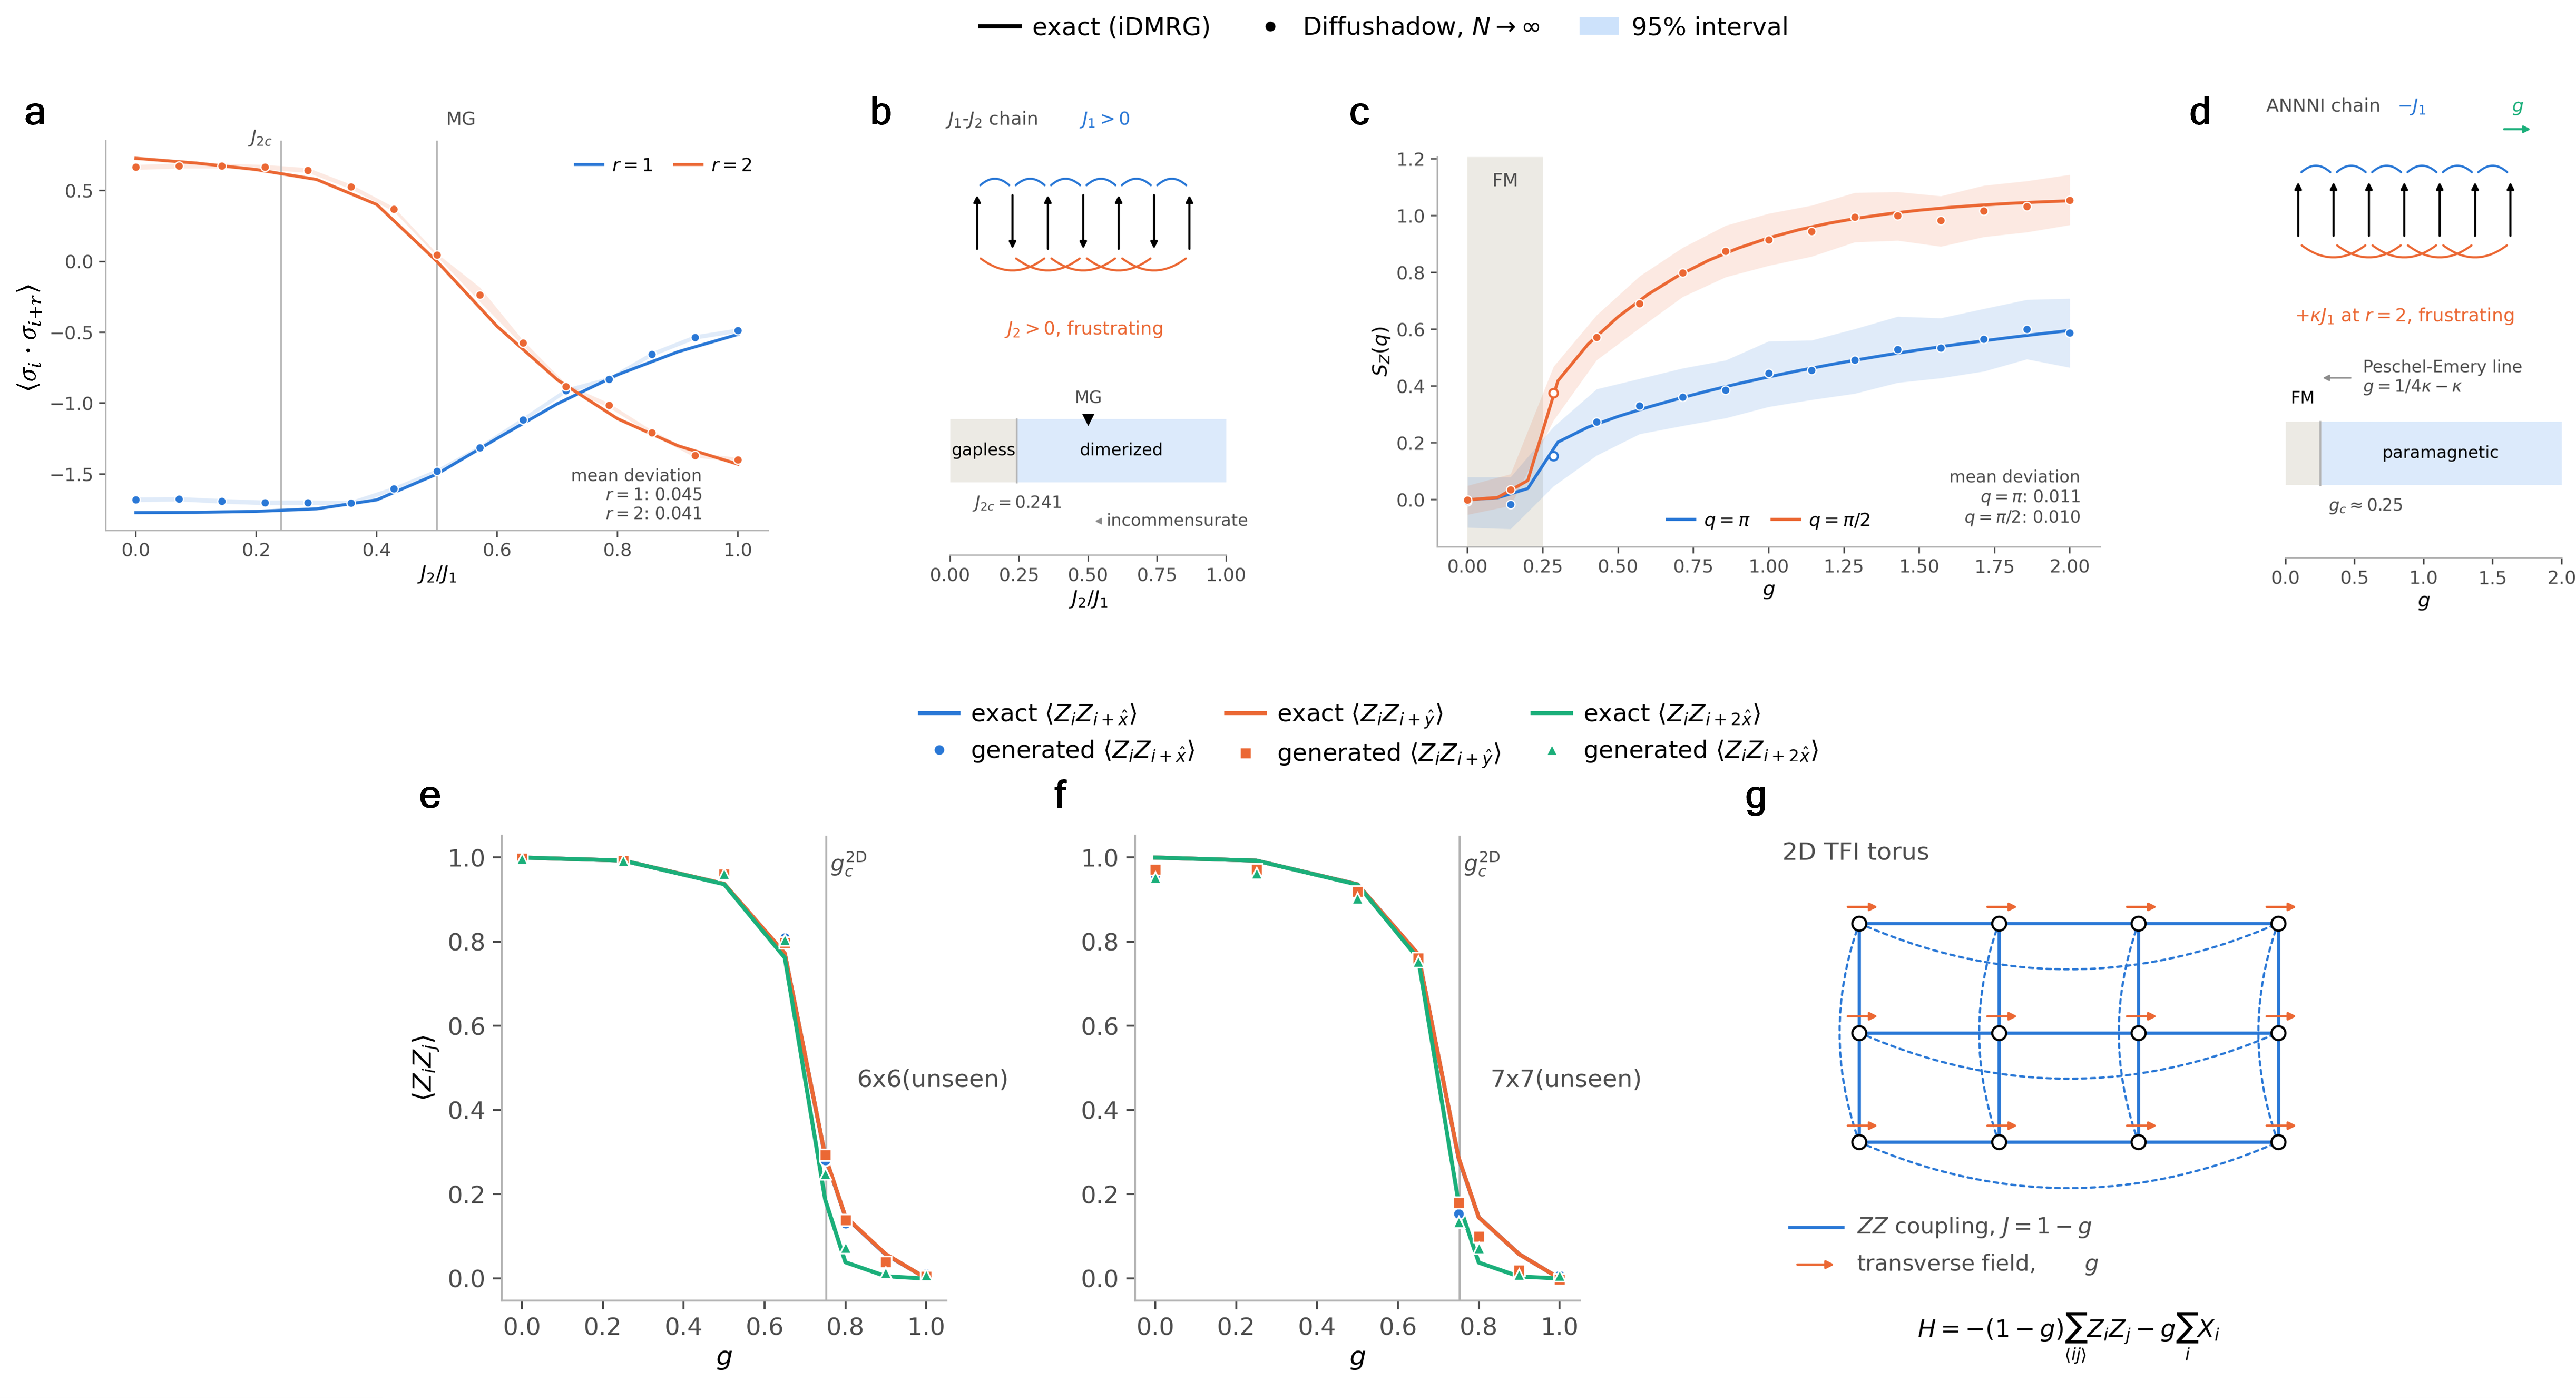
\includegraphics[width=\textwidth]{fig/FIG3_all3.2.png}
\caption{
\textbf{Thermodynamic-limit inference in frustrated spin chains and cross-scale generation on two-dimensional lattices.}
\textbf{a,} Thermodynamic-limit spin correlations $\langle\boldsymbol{\sigma}_i\cdot\boldsymbol{\sigma}_{i+r}\rangle$ for $r=1,2$ in the frustrated $J_1$--$J_2$ chain. Vertical lines mark the critical coupling $J_{2c}/J_1\approx0.241$ and the Majumdar--Ghosh (MG) point at $J_2/J_1=0.5$.
\textbf{b,} Interaction schematic and phase diagram of the $J_1$--$J_2$ chain, indicating the gapless and dimerized regimes, MG point and onset of incommensurate correlations.
\textbf{c,} Thermodynamic-limit longitudinal structure factors $S_Z(\pi)$ and $S_Z(\pi/2)$ in the ANNNI chain at $\kappa=0.4$. Grey shading indicates the ferromagnetic regime.
In a,c, solid curves show iDMRG references, and markers show Diffushadow estimates linearly extrapolated in $1/N$. Shading denotes pointwise 95\% bootstrap confidence intervals. Annotated mean absolute deviations exclude the open markers near the ANNNI transition in c.
\textbf{d,} Interaction schematic and phase diagram of the ANNNI chain, indicating the ferromagnetic and paramagnetic regimes.
\textbf{e,f,} Site-averaged $ZZ$ correlations on unseen $6\times6$ (e) and $7\times7$ (f) periodic TFI lattices, generated by a model trained on lattices of at most 16 spins. Solid curves show SSE quantum Monte Carlo references; markers show Diffushadow estimates. Blue circles, orange squares and green triangles denote horizontal nearest-neighbour $\langle Z_iZ_{i+\hat{x}}\rangle$, vertical nearest-neighbour $\langle Z_iZ_{i+\hat{y}}\rangle$ and horizontal next-nearest-neighbour $\langle Z_iZ_{i+2\hat{x}}\rangle$ correlations, respectively. Vertical lines mark $g_c^{\mathrm{2D}}\approx0.753$.
\textbf{g,} Periodic square-lattice geometry with nearest-neighbour $ZZ$ coupling $J=1-g$ (blue bonds) and transverse field $g$ (orange arrows). Dashed bonds indicate periodic connections.
}
\label{fig4}
\end{figure}



\subsection{Cross-scale generation across different Hamiltonians and lattice geometries}


% Through recursive scale extrapolation, the Diffushadow models trained across different rounds produce quantum many-body data at progressively larger system sizes. These data then enable the estimation of physical properties for quantum systems in the thermodynamic limit. Following the standard finite-size scaling paradigm in many-body physics, observables extracted from the generated measurements are analyzed as functions of the inverse system size $1/N$. Extrapolating the resulting scaling curves to $1/N=0$ provides estimates of their thermodynamic-limit values, allowing physical properties beyond the accessible finite-size regime to be inferred directly from Diffushadow-generated data.

% Having established cross-scale measurement generation and thermodynamic-limit inference in the one-dimensional TFI model, we next examine the applicability of Diffushadow to more complex interactions and lattice geometries. We consider the frustrated $J_1$--$J_2$ chain and the axial next-nearest-neighbour Ising (ANNNI) chain, which introduce competing interactions, and the two-dimensional TFI model on periodic square lattices. For each system, Diffushadow is trained on classical-shadow measurements from small systems and evaluated at larger unseen sizes. These benchmarks test whether the framework preserves model-specific correlation structures across scales and supports physical inference beyond the one-dimensional TFI setting.

We further evaluate Diffushadow on quantum systems with competing interactions and different lattice geometries. For the frustrated $J_1$--$J_2$ and axial next-nearest-neighbour Ising (ANNNI) chains, we use recursively generated measurements to estimate thermodynamic-limit observables. For the two-dimensional TFI model, we examine direct cross-scale generation on larger unseen periodic lattices without retraining.

% As shown in Fig. XX, the availability of large-scale quantum measurements generated through recursive scale extrapolation enables the construction of finite-size scaling curves over a substantially broader range of system sizes than would be accessible from exact data alone. For each correlation distance ($r$), spin-spin correlations $(\langle Z_i Z_{i+r}\rangle)$ estimated from both exact and generated measurements exhibit smooth and systematic dependence on the inverse system size ($1/N$). To capture the finite-size corrections and infer the corresponding thermodynamic-limit values, we fit the scaling curves using quadratic functions of ($1/N$) and extrapolate them to ($1/N=0$).

\subsubsection{Frustrated and competing-interaction spin chains}


% The $J_1$--$J_2$ and ANNNI chains provide two settings in which competing interactions produce correlation structures beyond those of the TFI model (Fig.~\ref{fig4}b,d). In the antiferromagnetic $J_1$--$J_2$ chain, competing nearest- and next-nearest-neighbour exchange interactions lead to a transition from a gapless regime to a dimerized regime at $J_{2c}/J_1\simeq0.241$, with the Majumdar--Ghosh (MG) point at $J_2/J_1=0.5$. We examine the spin-dot correlations $\langle\boldsymbol{\sigma}_i\cdot\boldsymbol{\sigma}_{i+r}\rangle$ at $r=1,2$, which probe the two competing exchange interactions. The ANNNI model combines ferromagnetic nearest-neighbour and competing next-nearest-neighbour Ising interactions in a transverse field. At $\kappa=0.4$, below the zero-field multiphase point $\kappa=0.5$, we evaluate the longitudinal structure factors $S_Z(\pi)$ and $S_Z(\pi/2)$, which probe staggered and period-four correlation components, respectively.

% For both models, measurement generation is evaluated at the training size $N=12$ and the unseen size $N=24$ (Supplementary Fig.~2). Recursively generated measurements at larger sizes are then used for empirical linear extrapolation in $1/N$, with the fitted intercepts compared against independent infinite-system density-matrix renormalization group (iDMRG) references. Pointwise 95\% bootstrap confidence intervals quantify finite-measurement sampling uncertainty propagated through observable estimation and extrapolation.


The antiferromagnetic $J_1$--$J_2$ chain features competing nearest- and next-nearest-neighbour exchange interactions, with a transition from the gapless to the dimerized regime at $J_{2c}/J_1\simeq0.241$ and the Majumdar--Ghosh (MG) point at $J_2/J_1=0.5$ (Fig.~\ref{fig4}b)~\cite{okamoto1992fluid, majumdar1969next2}. We probe these interactions through the spin-dot correlations $\langle\boldsymbol{\sigma}_i\cdot\boldsymbol{\sigma}_{i+r}\rangle$ at $r=1,2$. The ANNNI chain combines ferromagnetic nearest-neighbour and competing next-nearest-neighbour Ising interactions in a transverse field (Fig.~\ref{fig4}d)~\cite{beccaria2006density, chandra2007floating}. At $\kappa=0.4$, below the zero-field multiphase point $\kappa=0.5$, we examine $S_Z(\pi)$ and $S_Z(\pi/2)$, which probe staggered and period-four correlation components, respectively.

For both chains, we evaluate generated measurements at the training size $N=12$ and unseen size $N=24$ (Extended Data Fig.~\ref{fig:J1J2_ANNNI_12_24}), then extrapolate observables from recursively generated larger-size ensembles linearly in $1/N$. The intercepts are compared with independent infinite-system density-matrix renormalization group (iDMRG) references; pointwise 95\% bootstrap confidence intervals propagate finite-record sampling uncertainty through observable estimation and extrapolation.

In the $J_1$--$J_2$ chain, the spin-dot observable combines $XX$, $YY$ and $ZZ$ correlations, testing whether Diffushadow preserves statistics across Pauli components rather than only the longitudinal $ZZ$ correlations of the TFI model (Fig.~\ref{fig4}a). At weak frustration, nearest-neighbour correlations are strongly negative and next-nearest-neighbour correlations positive. As $J_2/J_1$ increases, Diffushadow captures the weakening of the former and the sign reversal of the latter near the MG point. At stronger frustration, it also reproduces the increasing magnitude of next-nearest-neighbour antiferromagnetic correlations relative to nearest-neighbour correlations. This redistribution across the gapless and dimerized regimes reflects the changing competition between exchange interactions. Mean absolute deviations from iDMRG are 0.045 ($r=1$) and 0.041 ($r=2$).

The ANNNI chain tests momentum-resolved structure factors, which combine longitudinal correlations across multiple spatial separations (Fig.~\ref{fig4}c). At $\kappa=0.4$, both $S_Z(\pi)$ and $S_Z(\pi/2)$ are small in the low-field ferromagnetic regime, where the dominant ordering wavevector is $q=0$. As the transverse field increases, Diffushadow reproduces the rapid rise and broad plateau of $S_Z(\pi/2)$, alongside the more gradual growth of $S_Z(\pi)$. Diffushadow also preserves the separation between the two profiles, including the greater spectral weight at $q=\pi/2$. Because the two wavevectors weight spatial separations differently, their simultaneous agreement with iDMRG indicates that the generated ensembles retain distinct components of the spatial correlation structure, not merely its overall magnitude. Mean absolute deviations from iDMRG are 0.011 and 0.010 for $S_Z(\pi)$ and $S_Z(\pi/2)$, respectively, excluding open markers near the transition where reference-grid interpolation is less reliable.


% In the $J_1$--$J_2$ chain, the two spin-dot correlations exhibit contrasting responses to increasing frustration (Fig.~\ref{fig4}a). At weak $J_2/J_1$, the nearest-neighbour correlation is strongly negative, reflecting antiferromagnetic correlations between adjacent spins, whereas the next-nearest-neighbour correlation is positive. As $J_2/J_1$ increases, the nearest-neighbour correlation becomes less negative, while the next-nearest-neighbour correlation decreases and changes sign. This redistribution of short-range correlations reflects the growing competition between the two exchange interactions. Diffushadow reproduces these trends across the gapless and dimerized regimes, including the region around the MG point (Fig.~\ref{fig4}b). The mean absolute deviations from the iDMRG references are 0.045 and 0.041 for $r=1$ and $r=2$, respectively.

% For the ANNNI chain, the thermodynamic-limit structure factors exhibit distinct responses to the transverse field (Fig.~\ref{fig4}c). Both $S_Z(\pi)$ and $S_Z(\pi/2)$ remain small in the low-field ferromagnetic regime, where longitudinal order is dominated by the uniform component. As the transverse field suppresses ferromagnetic order, $S_Z(\pi/2)$ increases rapidly and approaches a broad plateau, whereas $S_Z(\pi)$ grows more gradually. The different field dependences reflect the redistribution of longitudinal correlations among distinct spatial wavevectors in the presence of competing Ising interactions. Diffushadow reproduces both profiles, with mean absolute deviations of 0.011 and 0.010 for $S_Z(\pi)$ and $S_Z(\pi/2)$, respectively, excluding the open markers near the transition where interpolation of the iDMRG reference grid is less reliable.


% In the $J_1$--$J_2$ chain, we examine whether recursively generated measurements preserve the redistribution of spin correlations induced by competing exchange interactions (Fig.~\ref{fig4}a). Unlike the longitudinal $ZZ$ correlations evaluated in the TFI model, the spin-dot observable combines $XX$, $YY$ and $ZZ$ correlations, providing a test of measurement statistics across multiple Pauli components. At weak frustration, the nearest-neighbour correlation is strongly negative, whereas the next-nearest-neighbour correlation is positive. As $J_2/J_1$ increases, Diffushadow reproduces the weakening of nearest-neighbour antiferromagnetic correlations and the sign reversal of the next-nearest-neighbour correlation near the Majumdar--Ghosh point. At stronger frustration, the generated estimates also capture the increasing magnitude of the next-nearest-neighbour antiferromagnetic correlation relative to the nearest-neighbour contribution. This agreement extends across the gapless and dimerized regimes, indicating that the generated measurements retain the changing balance of correlations associated with the two competing exchange interactions. The mean absolute deviations from the iDMRG references are 0.045 and 0.041 for $r=1$ and $r=2$, respectively.

% The ANNNI model provides a complementary test through momentum-resolved structure factors, which combine longitudinal correlations over multiple spatial separations rather than probing a single distance. Figure~\ref{fig4}c compares the thermodynamic-limit estimates of $S_Z(\pi)$ and $S_Z(\pi/2)$ with iDMRG references at $\kappa=0.4$. Both structure factors remain small in the low-field ferromagnetic regime, where the ordering wavevector is $q=0$. The nonzero-wavevector components examined here respond differently as the transverse field increases. Diffushadow captures the rapid growth of $S_Z(\pi/2)$ beyond the ferromagnetic region and its approach to a broad plateau, while reproducing the more gradual increase of $S_Z(\pi)$. Importantly, the generated estimates preserve the separation between the two structure factors across the field range, including the stronger spectral weight at $q=\pi/2$. Because the two wavevectors weight spatial correlations differently, their simultaneous agreement with the references provides evidence that the generated measurement ensembles preserve distinct components of the spatial correlation structure. The mean absolute deviations are 0.011 and 0.010 for $S_Z(\pi)$ and $S_Z(\pi/2)$, respectively, excluding the open markers near the transition where interpolation of the iDMRG reference grid is less reliable.



% After establishing the full cross-scale generation and thermodynamic-limit inference pipeline in the transverse-field Ising model, we next examine whether Diffushadow can be extended beyond this canonical benchmark. 
% We consider two representative one-dimensional spin-chain Hamiltonians with competing interactions, the frustrated $J_1$--$J_2$ model (Fig.~\ref{fig3}e,f) and the axial next-nearest-neighbour Ising (ANNNI) model (Fig.~\ref{fig3}g,h). The $J_1$--$J_2$ model introduces competing nearest- and next-nearest-neighbour exchange interactions and exhibits frustration-induced dimerization physics, while the ANNNI model contains competing Ising interactions that give rise to modulated ordering tendencies. 
% % These models therefore provide a broader testbed for assessing whether Diffushadow can generate physically meaningful quantum measurement samples and support finite-size extrapolation beyond the transverse-field Ising setting.
% We evaluate model-specific observables that reflect the dominant correlations of the two Hamiltonians. For the $J_1$--$J_2$ model, we use the spin-dot correlations $\langle \boldsymbol{\sigma}_i \cdot \boldsymbol{\sigma}_{i+r}\rangle$ at $r=1,2$, which probe the nearest- and next-nearest-neighbour exchange interactions. For the ANNNI model at $\kappa=0.4$, we evaluate the structure factors $S_Z(\pi)$ and $S_Z(\pi/2)$, which characterize distinct longitudinal ordering components.

% We first consider two one-dimensional Hamiltonians with competing interactions. The $J_1$--$J_2$ chain combines antiferromagnetic nearest- and next-nearest-neighbour exchange interactions (Fig.~\ref{fig3}e), with a gapless regime at weak frustration and a dimerized regime above $J_{2c}/J_1\approx0.241$ (Fig.~\ref{fig3}f). We evaluate the spin-dot correlations $\langle \boldsymbol{\sigma}_i\cdot\boldsymbol{\sigma}_{i+r}\rangle$ at $r=1,2$, which directly probe the two exchange terms. The ANNNI chain combines ferromagnetic nearest-neighbour Ising interactions, frustrating next-nearest-neighbour interactions and a transverse field $h$ (Fig.~\ref{fig3}g). We fix the frustration ratio at $\kappa=0.4$ and evaluate the longitudinal structure factors $S_Z(\pi)$ and $S_Z(\pi/2)$. These observables probe distinct momentum components of the longitudinal correlations along a field-driven scan spanning the ferromagnetic and paramagnetic regimes (Fig.~\ref{fig3}h).
% The $J_1$--$J_2$ chain has also served as a representative benchmark for transformer-based variational wave functions ~\cite{viteritti2022accuracy,viteritti2023transformer}, more general neural-network quantum-state models~\cite{rende2025foundation}, and machine-learning analyses of its phase transition ~\cite{rahaman2023machine}. The ANNNI chain has likewise been studied using classical-shadow measurements combined with unsupervised learning to distinguish its ordered phases~\cite{morais2026distinguishing}, demonstrating that shadow-derived correlation features retain information about its ordering structure. These studies focus primarily on representing or optimizing quantum states or on identifying phase structure, with classical shadows used as features for downstream analysis. Here, we address a complementary question: whether a generative model trained only on small-system classical-shadow measurements can learn the randomized measurement distribution itself, transfer it to larger unseen system sizes, and support finite-size extrapolation. 
% The $J_1$--$J_2$ chain has also served as an important benchmark for machine-learning approaches to frustrated quantum systems ~\cite{rahaman2023machine,viteritti2022accuracy}. However, previous studies primarily focused on ground-state representation or phase characterization, whereas here we investigate the generation of classical-shadow measurement distributions and their scalability across system sizes.


% Since the characteristic physics of these Hamiltonians is different from that of the transverse-field Ising model, we evaluate model-specific observables that directly reflect their dominant interactions and ordering tendencies. For the $J_1$--$J_2$ model, we evaluate the spin-dot correlations $\langle \boldsymbol{\sigma}_i \cdot \boldsymbol{\sigma}_{i+r}\rangle$ at $r=1,2$ in both finite-size generation and thermodynamic-limit inference. These correlations directly probe the nearest- and next-nearest-neighbour exchange terms in the Hamiltonian. For the ANNNI model, we evaluate the structure factors \(S_Z(\pi)\) and \(S_Z(\pi/2)\), which probe distinct ordering tendencies associated with competing Ising interactions. In particular, \(S_Z(\pi/2)\) is sensitive to modulated ordering with period-four character, while \(S_Z(\pi)\) captures staggered ordering components. Throughout the ANNNI experiments, we fix the frustration ratio at $\kappa=0.4$. This value lies below the zero-field multiphase point $\kappa=0.5$, so the present scan probes field-driven behavior on the lower-frustration side rather than targeting the high-frustration floating or antiphase regime studied in canonical finite-size-scaling analyses~\cite{beccaria2007evidence,nagy2011exploring}. These observables therefore provide compact but physically meaningful tests of whether Diffushadow-generated measurements preserve the relevant correlation and ordering structures beyond the transverse-field Ising model.

% We first evaluate finite-size measurement generation for these two Hamiltonians. Figs.~\ref{fig3}a,b show the ANNNI results at 12 and 24 qubits, corresponding to same-size and cross-scale generation, respectively. The structure factors \(S_Z(\pi)\) and \(S_Z(\pi/2)\) estimated from Diffushadow-generated measurements are in good agreement with the exact results across the transverse-field parameter \(g\). For both system sizes, the generated measurements reproduce the distinct evolution of the two ordering components, including the rapid growth of \(S_Z(\pi/2)\) and the more gradual variation of \(S_Z(\pi)\). 
% Classical-shadow measurements have also recently been combined with unsupervised learning to distinguish ordered phases of the ANNNI
% chain~\cite{morais2026distinguishing}. That setting uses shadow-estimated
% correlation features for phase identification. Diffushadow instead
% models the randomized measurement distribution itself and evaluates
% whether the learned distribution can be transferred to larger unseen
% system sizes and used for finite-size extrapolation. 
% Figs.~\ref{fig3}c,d show the corresponding results for the $J_1$--$J_2$ model at 10 and 24 qubits, representing same-size and cross-scale generation, respectively. Diffushadow captures the main evolution of the spin-dot correlations at \(r=1,2,3\) as the frustration parameter \(J_2\) is varied, including the contrasting trends of correlations at different distances. These show that Diffushadow can generate measurement samples that preserve model-specific correlation and ordering structures not only at training system sizes, but also during cross-scale generation to larger spin chains.

% We first evaluate finite-size measurement generation for these two Hamiltonians. Figs.~\ref{fig3}a,b show the $J_1$--$J_2$ results at 12 and 24 qubits, corresponding to same-size and cross-scale generation, respectively. Diffushadow captures the main evolution of the spin-dot correlations at \(r=1,2\) as the frustration parameter \(J_2\) is varied, including the contrasting trends of the nearest- and next-nearest-neighbor correlations. Figs.~\ref{fig3}c,d show the corresponding ANNNI results at 12 and 24 qubits. The structure factors \(S_Z(\pi)\) and \(S_Z(\pi/2)\) estimated from Diffushadow-generated measurements are in good agreement with the exact finite-size results across the transverse-field parameter \(g\). At both system sizes, the generated measurements reproduce the distinct evolution of the two ordering components, including the rapid growth of \(S_Z(\pi/2)\) and the more gradual variation of \(S_Z(\pi)\). Together, these results show that Diffushadow-generated measurements preserve model-specific correlation and ordering structures both at the training system sizes and during cross-scale generation to larger spin chains.



% We examine whether the generated measurements for these more complex spin chains can also support finite-size extrapolation. Following the recursive scale-extrapolation strategy used for the transverse-field Ising model, we generate classical-shadow measurements for a sequence of larger system sizes and estimate the corresponding model-specific observables. These finite-size estimates are then analyzed as functions of \(1/N\) and extrapolated to \(1/N=0\), yielding thermodynamic-limit estimates for the selected observables.

% Finite-size generation tests at the training size $N=12$ and the unseen size $N=24$ show that Diffushadow reproduces the main parameter dependence of these model-specific observables (Supplementary Information). 
% We present the test results at the training size $N=12$ and the unseen size $N=24$ in Supplementary Fig.~2 and apply the recursive scale-extrapolation procedure to generate measurements for larger systems. Observable estimates extracted from these measurements are fitted linearly in $1/N$, with the intercepts providing thermodynamic-limit estimates. We compare these estimates with independent infinite-system density-matrix renormalization group (iDMRG) references. Bootstrap resampling propagates finite-measurement sampling uncertainty through the observable estimation and finite-size extrapolation.


% For the $J_1$--$J_2$ model, Figs.~\ref{fig3}a and \ref{fig3}b show the thermodynamic-limit estimates of the spin-dot correlations \(\langle \boldsymbol{\sigma}_i \cdot \boldsymbol{\sigma}_{i+r} \rangle\) for \(r=1\) and \(r=2\), respectively, as functions of \(J_2 / J_1\). These two correlation distances directly probe the nearest- and next-nearest-neighbour exchange terms in the Hamiltonian. As $J_2/J_1$ increases, the nearest-neighbour correlation becomes less negative, whereas the next-nearest-neighbour correlation decreases and changes sign. Diffushadow reproduces these contrasting trends, reflecting the competition between the two exchange interactions. Residual discrepancies are most apparent at weak frustration and are not fully captured by the bootstrap intervals, which quantify sampling uncertainty. 
% The shaded regions indicate 95\% bootstrap confidence intervals arising from finite measurement sampling and finite-size extrapolation. 
% Representative finite-size extrapolations at \(J_2=0.36\) and \(J_2=0.86\) are shown in Fig.~\ref{fig3}g. For both correlation distances, the estimates obtained from Diffushadow-generated measurements can be organized by linear fits in \(1/N\), with the fitted intercepts providing the corresponding thermodynamic-limit estimates.

% For the ANNNI model, Figs.~\ref{fig3}c and \ref{fig3}d show the thermodynamic-limit estimates of the structure factors \(S_Z(\pi)\) and \(S_Z(\pi/2)\), respectively, as functions of the transverse-field parameter \(g\). The generated estimates reproduce the distinct field dependence of the two structure factors. $S_Z(\pi/2)$ rises rapidly above the transition region and approaches a broad plateau, whereas $S_Z(\pi)$ increases more gradually. The mean absolute deviations from the iDMRG references are 0.011 and 0.010, respectively, excluding the open markers near the transition, where interpolation of the reference grid is less reliable. 
% Representative finite-size extrapolations at \(g=0.71\) and \(g=1.71\) are shown in Fig.~\ref{fig3}j. For both structure factors, the estimates obtained from Diffushadow-generated measurements can be organized by linear fits in \(1/N\), with the fitted intercepts providing the corresponding thermodynamic-limit estimates. These results can be viewed as an observable-level finite-size analysis at fixed \(\kappa=0.4\), rather than as a reconstruction of the complete ANNNI phase diagram~\cite{beccaria2007evidence,nagy2011exploring}.



% Together, these results extend the thermodynamic-limit inference pipeline beyond the transverse-field Ising benchmark. Although the frustrated $J_1$-$J_2$ and ANNNI models exhibit more complex finite-size behavior, Diffushadow-generated measurements still preserve the relevant model-specific correlation and ordering structures across system sizes. This supports the use of Diffushadow as a flexible measurement-generation framework for finite-size extrapolation in one-dimensional spin-chain systems with competing interactions.

% Together, these results extend thermodynamic-limit inference beyond the transverse-field Ising benchmark to spin chains with competing interactions. 
% % Diffushadow-generated measurements preserve the characteristic parameter dependence of the selected correlation observables across system sizes and support their finite-size extrapolation. 
% % This supports the use of Diffushadow as a flexible measurement-generation framework for finite-size extrapolation in one-dimensional spin-chain systems with competing interactions.
% This shows that recursively generated measurement ensembles can preserve model-specific finite-size trends across distinct one-dimensional Hamiltonians.


\subsubsection{Cross-scale generation on two-dimensional lattices}


% Figures~\ref{fig3}c,d show the corresponding results for the $J_1$--$J_2$ model at 10 and 24 qubits, representing same-size and cross-scale generation, respectively. We evaluate the spin-dot correlations \(\langle \boldsymbol{\sigma}_i\cdot\boldsymbol{\sigma}_{i+r}\rangle\) at distances \(r=1,2,3\). As the frustration parameter \(J_2\) increases, the nearest-neighbor correlation becomes less negative, while the next-nearest-neighbor correlation decreases and changes sign. The third-neighbor correlation exhibits an opposite trend, increasing from negative to positive values. Diffushadow-generated measurements reproduce these distance-dependent trends in both the trained-size and cross-scale settings, indicating that the model can capture the redistribution of spin correlations induced by competing exchange interactions.
% We next test whether cross-scale generation persists when the lattice geometry changes from one to two dimensions. This setting further motivates generation without a fixed causal ordering, as no single linear ordering preserves local adjacency uniformly along both spatial directions. Under a fixed autoregressive ordering, each outcome prediction is restricted to preceding outcomes, irrespective of their spatial relationship to the target site. Full-attention iterative denoising instead allows masked outcomes to condition on available measurement information throughout the lattice. 
% % We therefore examine the two-dimensional transverse-field Ising model to assess whether Diffushadow can generate measurements that preserve spatial correlations at larger, unseen lattice sizes.

% % We next extend Diffushadow to two-dimensional lattices, where no single linear ordering preserves local adjacency along both spatial directions. Full-attention denoising allows masked outcomes to condition on available measurements throughout the lattice, motivating its use for cross-scale generation in the two-dimensional transverse-field Ising model.

% We consider the two-dimensional TFI model on square lattices with periodic boundary conditions (Fig.~\ref{fig3}k). Diffushadow is trained on classical-shadow measurements from a mixture of small two-dimensional lattices containing at most 16 spins, with two-dimensional rotary positional embeddings encoding lattice coordinates. Without further training, the model generates measurement snapshots for unseen \(6\times6\) and \(7\times7\) lattices. We evaluate site-averaged horizontal and vertical nearest-neighbour \(ZZ\) correlations and horizontal next-nearest-neighbour correlations estimated from generated snapshots against stochastic series expansion quantum Monte Carlo (SSE QMC) references.

% Diffushadow is trained on classical-shadow measurements from periodic square lattices containing at most 16 spins, with two-dimensional rotary positional embeddings encoding lattice coordinates (Fig.~\ref{fig3}k). Without further training, the model generates measurement snapshots for unseen \(6\times6\) and \(7\times7\) lattices. We evaluate site-averaged horizontal and vertical nearest-neighbour \(ZZ\) correlations and horizontal next-nearest-neighbour correlations estimated from generated snapshots against stochastic series expansion quantum Monte Carlo (SSE QMC) references.

% Figs.~\ref{fig3}i,j compare correlations estimated from Diffushadow-generated measurements with SSE QMC reference results for the unseen \(6\times6\) and \(7\times7\) lattices. Across the scanned range of \(g\), the generated estimates closely follow the reference curves, reproducing the strong longitudinal correlations in the interaction-dominated regime and their suppression as the transverse field increases. This agreement is observed in both horizontal and vertical nearest-neighbour correlations, showing that the generated measurements recover the tested local correlations along both spatial directions. The horizontal next-nearest-neighbour correlations also follow the reference trend, extending the agreement to sites separated by more than one lattice spacing. All three observables are estimated from the same ensemble of generated classical-shadow snapshots, providing a common measurement representation for assessing correlations across directions and distances. The correspondence persists on the \(7\times7\) lattice, containing approximately three times as many spins as the largest training system, demonstrating that the tested spatial correlation structure remains accessible through generated measurements well beyond the training sizes.

% As shown in Figs.~\ref{fig3}i,j, the generated estimates closely follow the SSE QMC results across the scanned values of \(g\), reproducing the suppression of longitudinal correlations with increasing transverse field. This agreement is observed in both horizontal and vertical nearest-neighbour correlations, showing that the generated measurements recover the tested local correlations along both spatial directions. The horizontal next-nearest-neighbour correlations also follow the reference trend, extending the agreement to sites separated by more than one lattice spacing. The correspondence persists on the \(7\times7\) lattice, which contains approximately three times as many spins as the largest training system.

% These results demonstrate cross-scale measurement generation on two-dimensional lattices, with model trained on systems of at most 16 spins preserving the tested spatial correlations on unseen 36- and 49-spin lattices. Together with the $J_1$--$J_2$ and ANNNI results, they show that the framework can generate measurements for larger unseen systems across settings with competing interactions and different lattice geometries, while retaining the model-specific correlations and ordering signatures assessed here.



We evaluate direct cross-scale generation in the two-dimensional TFI model on periodic square lattices, where nearest-neighbour $ZZ$ interactions couple spins along both spatial directions and periodic bonds connect opposite lattice boundaries (Fig.~\ref{fig4}g). Unlike one-dimensional chains, these two-dimensional neighbour relationships cannot be represented uniformly as local adjacency under a fixed linear ordering. We train a separate Diffushadow model on classical-shadow measurements from mixed-size two-dimensional lattices containing at most 16 spins, using two-dimensional rotary positional embeddings to encode lattice coordinates. Without retraining, the model generates measurement records for unseen $6\times6$ and $7\times7$ lattices, containing 36 and 49 spins, respectively. We compare site-averaged horizontal and vertical nearest-neighbour $ZZ$ correlations, together with horizontal next-nearest-neighbour correlations, against stochastic series expansion quantum Monte Carlo (SSE QMC) references.

% We evaluate direct cross-scale generation in the two-dimensional TFI model on periodic square lattices, with nearest-neighbour $ZZ$ interactions along both spatial directions (Fig.~\ref{fig4}g). Because a fixed linear ordering cannot preserve local adjacency along both lattice axes, we use two-dimensional rotary positional embeddings to encode lattice coordinates. A separate Diffushadow model trained on mixed-size classical-shadow measurements from lattices of at most 16 spins generates records for unseen $6\times6$ and $7\times7$ lattices (36 and 49 spins) without retraining. We compare site-averaged horizontal and vertical nearest-neighbour $ZZ$ correlations and horizontal next-nearest-neighbour correlations with finite-size stochastic series expansion quantum Monte Carlo (SSE QMC) references.

Figures~\ref{fig4}e,f show that Diffushadow closely reproduces the SSE QMC correlations on both unseen lattice sizes. The periodic square geometry gives equivalent local environments along the horizontal and vertical directions, for which the exact nearest-neighbour correlations are equal by lattice symmetry. Diffushadow recovers this near-equivalence in its generated measurements while accurately following the field dependence of both directional correlations. The model also reproduces the distinct behaviour of horizontal next-nearest-neighbour correlations, which are more strongly suppressed than nearest-neighbour correlations as the transverse field increases. The agreement across different spatial directions and separations indicates that the generated measurements preserve the tested directional symmetry and distance-dependent correlation structure beyond the training sizes.

Near the two-dimensional critical coupling $g_c^{2D}\simeq0.753$, Diffushadow captures the rapid suppression of longitudinal correlations on both unseen lattice sizes, including the different rates of decay of nearest- and next-nearest-neighbour correlations (Fig.~\ref{fig4}e,f). The SSE QMC references also exhibit visible finite-size differences between the $6\times6$ and $7\times7$ lattices in this region. Diffushadow follows these size-dependent variations rather than reproducing identical correlation profiles at the two sizes, although deviations from the references remain near the transition. Notably, this agreement extends to the unseen $7\times7$ lattice, containing 49 spins compared with at most 16 in training. The results show that direct cross-scale generation preserves the tested spatial correlations and their finite-size dependence across substantially larger two-dimensional lattices, without retraining or recursive scale extrapolation.



\begin{figure}[ht!]
\centering
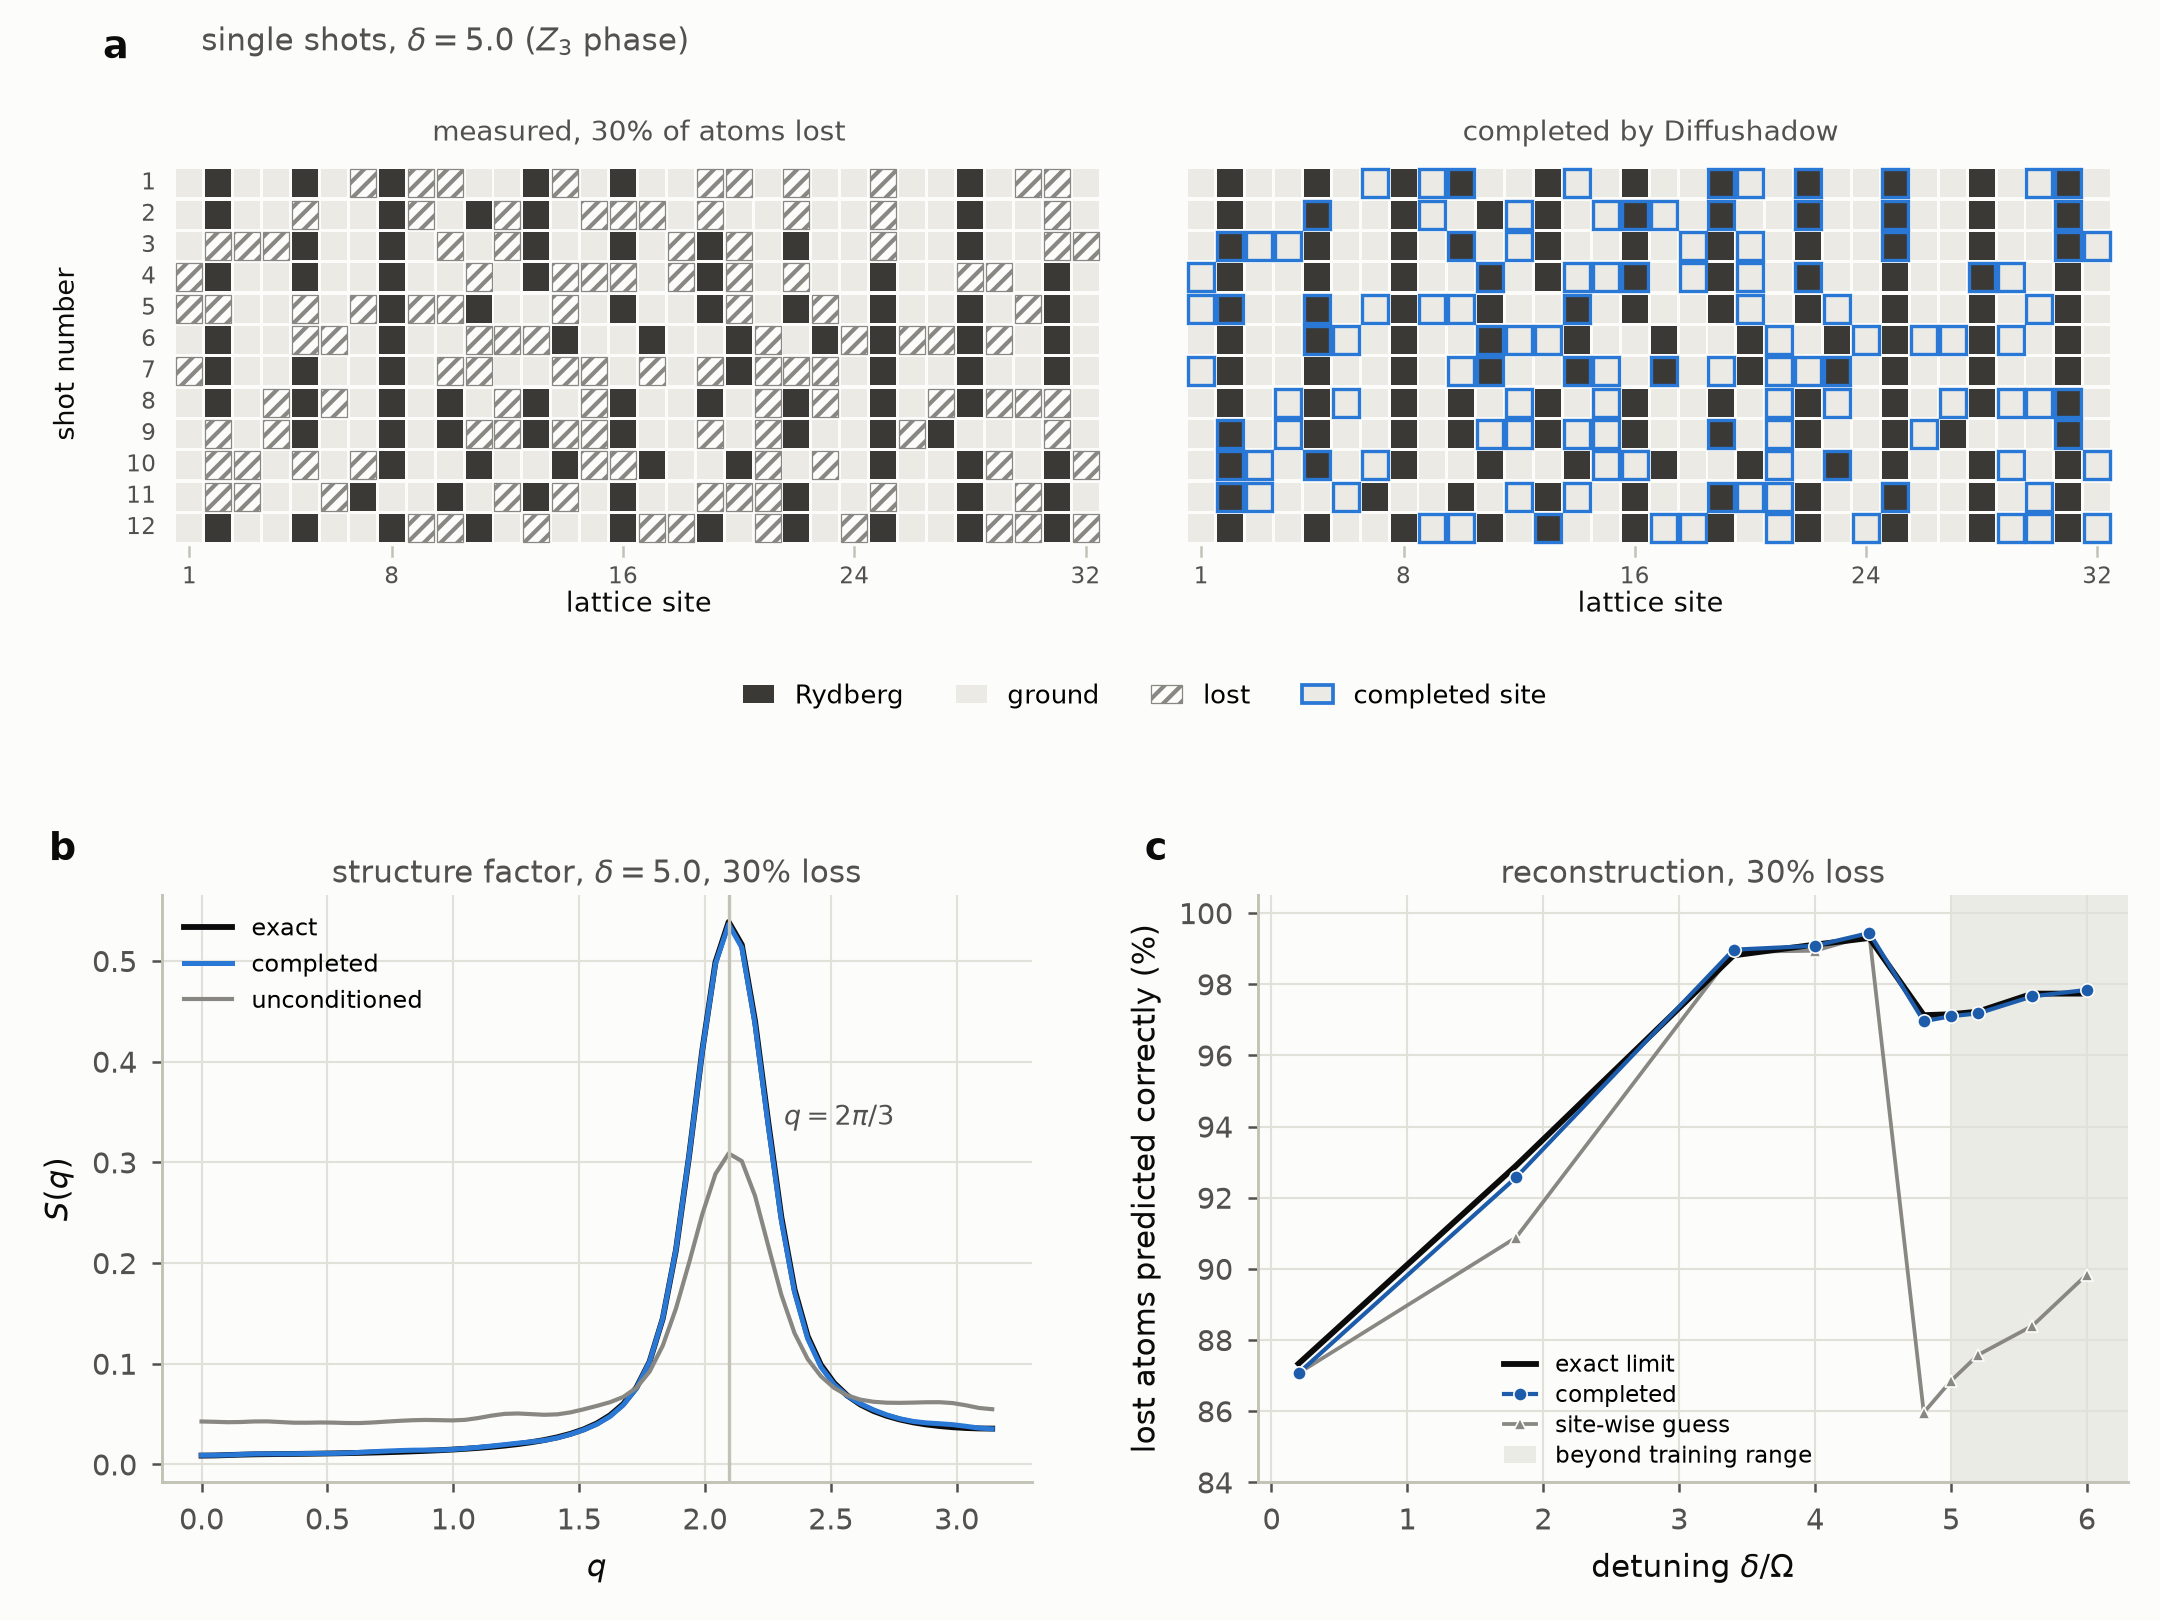
\includegraphics[width=0.98\textwidth]{fig/FIG5_rydberg_v2.png}
\caption{\textbf{Reconstruction of incomplete Rydberg measurement records.} Results for an open chain of $N=32$ atoms at blockade radius $R_b/a=2.35$, using held-out occupation snapshots sampled from DMRG ground states. Missing readouts are simulated by randomly masking 30\% of the sites in each snapshot. Diffushadow reconstructs the masked outcomes by conditional denoising while keeping observed outcomes fixed. \textbf{a,} Twelve partially observed snapshots at $\delta/\Omega=5.0$ (left) and their conditional completions (right). Dark and light cells denote Rydberg and ground-state occupations, respectively; hatched cells indicate missing readouts, and blue outlines identify completed sites. \textbf{b,} Connected density--density structure factor $S(q)$ at the same detuning. Black, blue and grey curves show the DMRG reference, conditionally completed ensemble and unconditioned-fill control, respectively. The control fills missing sites using model samples conditioned only on detuning. The vertical line marks the $Z_3$ correlation peak at $q=2\pi/3$. Panels \textbf{a,b} use conditional sampling. \textbf{c,} Prediction accuracy at masked sites as a function of $\delta/\Omega$, using deterministic decoding (blue circles). The black curve shows the Bayes-optimal per-site accuracy computed from conditional marginals of the DMRG reference state. Grey triangles show a site-wise baseline that predicts the more probable occupation from each site's unconditional density. The shaded region indicates detunings beyond the training range, $\delta/\Omega>5.0$. Within each comparison, the same missing-site masks are used for Diffushadow and the corresponding references or controls.
}
\label{fig5}

\end{figure}


\subsection{Reconstruction of incomplete Rydberg measurement records}

% \subsection{Learning physically aligned quantum structures}

% % Although Diffushadow exhibits promising performance in generalizing towards large-scale quantum systems, a crucial question remains: Does Diffushadow genuinely comprehend the physical implications of the many-body system and learn transferable quantum structures?

% Although Diffushadow exhibits strong performance in modeling and generalizing quantum measurement distributions across system sizes, it remains important to ask whether its cross-scale behavior is supported by physically meaningful internal structures rather than by memorization of finite-size statistical patterns. We investigate this question in the transverse-field Ising model, which provides a controlled setting with well-characterized phases and exact spin-spin correlation profiles. Through attention analysis, we investigate the internal structures learned by the model \cite{clark2019does}, thereby providing a mechanistic perspective on Diffushadow's scale generalization. 



% We first quantify the spatial range of attention by measuring the attention-weighted site distance from masked measurement queries to site-indexed tokens. Specifically, we compute the average distance between a masked measurement token and the sites it attends to, weighted by attention scores and averaged over all masked queries, heads and layers. Here, site-indexed tokens include both measurement-basis tokens $P_i$ and measurement-outcome tokens $b_i$. Intuitively, this quantity measures the effective spatial receptive field of the model. Higher values indicate that information is aggregated from more distant sites, whereas lower values imply a stronger reliance on local neighborhoods. As shown in Fig. \ref{fig4}a, the normalized mean site distance varies systematically with the coupling parameter, indicating that the model adapts its spatial receptive field across physical regimes. Moreover, it remains consistently larger in the ordered regime ($g<0.5$) than in the paramagnetic regime ($g>0.5$) across all system sizes. This trend is consistent with the physical characteristics of the one-dimensional transverse-field Ising model, where the ferromagnetic phase is associated with stronger and more extended spatial correlations, while correlations become increasingly short-ranged in the paramagnetic phase. Notably, the curves retain a highly consistent shape across system sizes, indicating that the model captures some degree of scale invariance in the underlying quantum system.



% Beyond generating new measurement records, Diffushadow can also reconstruct missing outcomes in partially observed records. In experiments on programmable atom arrays, some atoms may be lost or their readouts may be unavailable, leaving individual measurement records incomplete. Discarding these records reduces the number of samples available for estimating multisite observables, even though the observed sites still contain useful information about the underlying correlation structure. Also, requiring complete readouts at all sites involved in an observable becomes increasingly restrictive as the number of sites grows, increasing the measurement resources needed for statistical estimation. However, incomplete records still contain useful information because correlations between observed and unobserved sites constrain the possible missing outcomes. This conditional information provides a basis for retaining partially observed records through reconstruction.
% Measurements from programmable atom arrays can be incomplete when atoms are lost from the trap, and detection assigns no outcome at the affected sites.  The standard response is to discard incomplete shots, which becomes prohibitive for observables that involve many sites at once. It reduces the number of samples available for estimating multisite observables, even though the observed sites still contain useful information about the underlying correlation structure. This conditional information can provide a basis for retaining partially observed records through reconstruction.
% By learning the joint measurement distribution, Diffushadow provides a conditional reconstruction procedure that holds observed outcomes fixed and fills missing positions through iterative denoising. This application uses the trained model without additional training or architectural modifications.

% Measurements from programmable atom arrays can be incomplete when atoms are lost from the trap or when readout fails at individual sites, leaving the affected positions without recorded outcomes. A common response is to discard incomplete shots, which can substantially reduce the number of usable samples for multisite observables that require all relevant sites to be observed. Yet the remaining outcomes still contain conditional information about the missing sites. The masked-denoising formulation of Diffushadow provides a direct way to exploit this information by holding observed outcomes fixed while reconstructing missing positions through iterative denoising. This conditional reconstruction uses the same trained model as measurement generation, without task-specific retraining or architectural modification.

% Measurements from programmable atom arrays can be incomplete owing to atom loss or readout failure, reducing the number of records usable for multisite observables. Diffushadow addresses this setting by holding observed outcomes fixed while reconstructing missing positions through iterative denoising, using the same trained model as for measurement generation without task-specific retraining.




Measurements from programmable atom arrays can be incomplete owing to atom loss or readout failure, reducing the number of records usable for multisite observables. In Rydberg systems, spatial occupation correlations and blockade constraints provide information about missing outcomes through the remaining observations. Diffushadow exploits this conditional information by holding observed outcomes fixed while reconstructing missing positions through iterative denoising, without task-specific retraining. We evaluate this capability on an open Rydberg chain of $N=32$ atoms at blockade radius $R_b/a=2.35$, using held-out occupation snapshots sampled from DMRG ground states. The model is trained on chains with $N=16,24,32$, and 30\% of the sites are randomly masked at test time. Conditional sampling is used to reconstruct measurement ensembles, whereas deterministic decoding predicts individual missing outcomes (Fig.~\ref{fig5}a).

We first assess whether the reconstructed ensembles preserve collective spatial correlations. At $\delta/\Omega=5.0$, Diffushadow recovers the characteristic $Z_3$ peak of the connected density--density structure factor at $q=2\pi/3$, with an amplitude of 0.536 compared with the DMRG reference value of 0.539 (Fig.~\ref{fig5}b). In contrast, an unconditioned-fill control, which inserts occupations from independently generated records conditioned only on detuning, produces a substantially reduced peak of 0.309. This difference shows the importance of conditioning on the observed occupations of each individual record. By incorporating these observations, Diffushadow recovers the spatially organized correlations that are substantially weakened when missing sites are filled without regard to their measurement context.

Conditional completion also preserves local physical consistency between observed and reconstructed sites. Across the tested detunings, the fraction of doubly excited nearest-neighbour pairs spanning these sites remains below 0.02\%, compared with up to 3.7\% for the unconditioned-fill control (Supplementary Information). This low violation rate is achieved without explicitly enforcing blockade constraints during decoding, indicating that the learned conditional measurement statistics retain the local restrictions associated with Rydberg interactions. The reconstruction further supports multisite observable estimation. At $\delta/\Omega=5.0$, Diffushadow reproduces intact-data estimates of two- and eight-site occupation correlators, evaluated at sites separated according to the $Z_3$ period, to within approximately 0.002. Meanwhile, the average numbers of usable records increase from 467 and 28, respectively, to all 1000 test records (Supplementary Information). Thus, conditional reconstruction enables substantially more incomplete records to contribute to multisite correlation estimates while maintaining close agreement with the corresponding intact-data observables.

For individual-outcome prediction, we compare deterministic Diffushadow decoding with the Bayes-optimal expected per-site accuracy obtained from conditional occupation marginals of the reference DMRG matrix product state (Fig.~\ref{fig5}c). These marginals account for the same observed occupations available to Diffushadow and define the optimal expected accuracy for predicting each missing site. We also evaluate an unconditional site-density baseline that predicts the most probable occupation at each position without conditioning on the observed record. At $\delta/\Omega=5.0$, Diffushadow achieves 97.1\% accuracy, closely approaching the Bayes-optimal reference of 97.2\% and substantially exceeding the baseline accuracy of 86.9\%. The model remains close to the Bayes-optimal reference across the tested detunings, including $\delta/\Omega=5.2,5.6,6.0$ beyond the training range $\delta/\Omega\leq5.0$. This agreement indicates that Diffushadow effectively exploits the conditional information in partially observed records for missing-site prediction, with the learned conditional statistics remaining useful even at unseen detunings.


% We evaluate reconstruction on an open Rydberg chain of $N=32$ atoms at blockade radius $R_b/a=2.35$, using held-out occupation snapshots sampled from DMRG ground states. The model is trained on chains with $N=16,24,32$, and 30\% of the sites are randomly masked at test time. We use conditional sampling to reconstruct measurement ensembles and deterministic decoding to predict individual missing outcomes (Fig.~\ref{fig4}a).

% The conditionally completed ensembles retain the characteristic spatial correlations of the reference state. At $\delta/\Omega=5.0$, the connected density--density structure factor preserves the $Z_3$ peak at $q=2\pi/3$, with amplitude 0.536 compared with the DMRG reference value of 0.539 (Fig.~\ref{fig4}b). An unconditioned-fill control, which inserts model samples generated from detuning alone into the missing positions, yields a reduced peak of 0.309. These comparisons demonstrate the importance of conditioning on the observed outcomes of each individual record. Consistent with this preservation of spatial correlations, the fraction of doubly excited nearest-neighbour pairs spanning observed and reconstructed sites remains below 0.02\% across the tested detunings, without explicitly enforcing the blockade during decoding. The corresponding fraction reaches 3.7\% for the unconditioned-fill control (Supplementary Information).

% The benefit of reconstruction also extends to multisite observable estimation. At $\delta/\Omega=5.0$ and 30\% missing readouts, conditional completion reproduces the intact-data estimates of two- and eight-site occupation correlators, with sites separated by the $Z_3$ period, to approximately 0.002. Compared with retaining only records in which every required site is observed, completion increases the usable sample from an average of 467 and 28 records, respectively, to all 1000 test records (Supplementary Information). These results illustrate how reconstruction can retain information for observables whose evaluation would otherwise exclude a large fraction of partially observed measurements.

% To assess individual-outcome prediction, we compute the conditional occupation marginals of the missing sites from the DMRG matrix product state. These marginals determine the Bayes-optimal expected per-site accuracy given the same observed outcomes. Figure~\ref{fig4}c compares this reference with deterministic Diffushadow decoding and a site-wise baseline that predicts each site's more probable occupation from its unconditional density. Diffushadow closely approaches the Bayes-optimal accuracy across the tested detunings, including $\delta/\Omega=5.2,5.6,6.0$, beyond the training range $\delta/\Omega\leq5.0$. The advantage over the site-wise baseline becomes pronounced at larger detunings. At $\delta/\Omega=5.0$, the reconstruction accuracy is 97.1\%, compared with the Bayes-optimal value of 97.2\% and the baseline accuracy of 86.9\%.


% We evaluate reconstruction on an open Rydberg chain of $N=32$ atoms at blockade radius $R_b/a=2.35$, using held-out occupation snapshots sampled from DMRG ground states. The model is trained on chains with $N=16,24,32$, and 30\% of the sites are randomly masked at test time. Conditional sampling is used to reconstruct measurement ensembles, whereas deterministic decoding predicts individual missing outcomes (Fig.~\ref{fig4}a).

% Conditional completion preserves the spatial correlations of the reference state. At $\delta/\Omega=5.0$, the connected density--density structure factor preserves the $Z_3$ peak at $q=2\pi/3$ with amplitude 0.536, close to the DMRG reference value of 0.539, whereas an unconditioned-fill control yields 0.309 (Fig.~\ref{fig4}b). The fraction of doubly excited nearest-neighbour pairs spanning observed and reconstructed sites remains below 0.02\% across the tested detunings, compared with up to 3.7\% for the unconditioned-fill control (Supplementary Information). Conditional completion also reproduces the intact-data estimates of two- and eight-site occupation correlators to within approximately 0.002, while increasing the corresponding average numbers of usable records from 467 and 28 to all 1000 test records (Supplementary Information).

% For individual-outcome prediction, we compare deterministic decoding with the Bayes-optimal expected per-site accuracy derived from the reference DMRG state and with an unconditional site-density baseline. Diffushadow closely approaches the Bayes-optimal accuracy across the tested detunings, including $\delta/\Omega=5.2,5.6,6.0$ beyond the training range $\delta/\Omega\leq5.0$ (Fig.~\ref{fig4}c). At $\delta/\Omega=5.0$, its accuracy is 97.1\%, compared with 97.2\% for the Bayes-optimal reference and 86.9\% for the baseline.

% % Together, these results demonstrate an application of Diffushadow to incomplete measurement records, combining recovery of ensemble correlation statistics with accurate prediction of missing site occupations. These capabilities broaden the use of Diffushadow from generating new measurements to reconstructing partially observed datasets, without additional training or architectural modifications. This provides a practical way to make fuller use of the measurements that would otherwise contribute less, or be discarded entirely, in analyses of multisite observables.

% Together, these results show that Diffushadow recovers both ensemble-level correlations and individual missing outcomes from incomplete Rydberg measurements without additional training. This provides a practical way to make fuller use of the measurements that would otherwise contribute less, or be discarded entirely, in analyses of multisite observables.



% Together, these results demonstrate that the same denoising framework used for measurement generation can also recover information from incomplete Rydberg records without task-specific retraining. Conditional sampling preserves ensemble-level correlation statistics, while deterministic decoding approaches the Bayes-optimal per-site prediction accuracy. This reconstruction capability provides a practical way to make fuller use of partially observed measurements that would otherwise contribute less, or be discarded entirely, in analyses of multisite observables.




 
% To further resolve the spatial structure of attention, we construct site-resolved attention kernels for measurement-basis tokens and measurement-outcome tokens. These kernels characterize how attention is distributed across different token types and lattice distances.
% Specifically, the attention kernel $K(r, g)$ is defined as the average attention mass assigned to tokens located $r$ lattice sites away from a masked measurement query when the Hamiltonian parameter is $g$. 
% % The kernel therefore characterizes how attention is distributed as a function of spatial separation and Hamiltonian parameter $g$. 
% Depending on the token type of the attended keys, the kernel can be further decomposed into outcome-directed kernels $K_{bb}(r, g)$ and basis-directed kernels $K_{bP}(r, g)$, corresponding to attention allocated to measurement-outcome tokens and measurement-basis tokens, respectively. Figs. \ref{fig4}b and c show how much attention a masked measurement token assigns to measurement-outcome tokens and measurement-basis tokens at different lattice distances, respectively.
% Fig. \ref{fig4}b reveals a pronounced concentration of attention at distances 0 and 1 across all coupling strengths. Beyond these local interactions, a clear phase-dependent pattern emerges. For $g<0.5$, substantial attention mass persists over a broad range of distances, leading to a relatively slow spatial decay and enhanced long-range information aggregation. In contrast, for $g>0.5$, attention becomes strongly localized, with distances 0 and 1 dominating the distribution and attention rapidly diminishing at larger separations. This behavior is consistent with the stronger long-range correlations present in the ferromagnetic phase of the transverse-field Ising model.
% In Fig. \ref{fig4}c, the attention mass is overwhelmingly concentrated at distance 0, far exceeding that at all other distances. This indicates that Diffushadow primarily relies on the measurement basis of the same site when predicting a masked measurement outcome, consistent with the fact that the local measurement basis provides the most direct information about the corresponding measurement result.


% % For a masked measurement query token \(b_i\), we define a site-resolved attention kernel by aggregating attention over all key tokens of type
% % \(\tau \in \{P,b\}\) at relative site displacement \(r\):
% % \[
% % K_{\tau}(r;g)
% % =
% % \left\langle
% % \sum_{j}
% % A(b_i,\tau_j)\,
% % \mathbf{1}\!\left[j-i=r\right]
% % \right\rangle_{i,\mathrm{prompts}},
% % \qquad \tau \in \{P,b\}.
% % \]
% % where \(A_{\ell h}(q_i,\tau_j \mid g,N)\) is the attention weight in layer \(\ell\) and head \(h\) from the query token \(q_i=b_i\) to the key token \(\tau_j\), \(\mathcal{Q}\) denotes the set of masked measurement queries averaged over prompts and sites, and \(d(j,i)\) is the signed site displacement from query site \(i\) to key site \(j\) under periodic boundary conditions.

% While the preceding analyses characterize the average attention behavior of the model, these aggregate statistics may conceal substantial heterogeneity across individual attention heads. We therefore examine the spatial attention patterns of individual heads. As shown in Fig. \ref{fig4}d, we further probe the sensitivity of individual attention heads by quantifying how their attention patterns vary with the coupling parameter $g$. While attention heads in the first two layers remain largely invariant across different values of $g$, heads in deeper layers exhibit substantially stronger responses to changes in the physical regime. Such head-dependent behavior suggests a degree of functional specialization within the model, with different attention heads responding to different aspects of the underlying quantum correlations \cite{voita2019analyzing, michel2019sixteen}. This observation naturally raises the question of whether these specialized heads encode physically meaningful correlation structures. 

% To investigate this possibility, we compare the spatial attention kernel of representative specialized heads with the exact correlation profile of the underlying quantum system. For this purpose, we introduce an absolute-distance attention kernel $K(\lvert r \rvert)$, obtained by combining attention weights associated with separations $+r$ and $-r$. As shown in Fig. \ref{fig4}e, the attention kernel of a representative specialized head (L5H4) closely matches the corresponding correlation profile $\langle Z_i Z_{i+r}\rangle$ when $g=0.7$. The resulting cosine similarity reaches 0.975, indicating that, for this representative head and parameter setting, the spatial organization of attention is strongly aligned with the physical correlation structure encoded in the quantum state.
% To further quantify the relationship between attention and physical correlations, we compare the characteristic spatial scales of the attention kernel and the correlation profile. Specifically, we compute the attention-weighted mean distance from the normalized kernel $K(\lvert r \rvert)$ and the correlation-weighted mean distance from the normalized correlation profile $\langle Z_i Z_{i+r}\rangle$. Fig. \ref{fig4}f shows the resulting relationship for the specialized attention head L5H2 across different coupling parameters $g$. A strong linear correlation is observed (Pearson’s $\rho = 0.943$), indicating that this attention head's effective receptive field varies systematically with the spatial extent of the physical correlations present in the quantum state.

% While Figs. \ref{fig4}e and \ref{fig4}f provide evidence from representative specialized heads, it remains important to assess whether the observed alignment persists across different physical regimes and system sizes. To characterize the model's behavior, we computed the cosine similarity between the attention kernel of each attention head and the corresponding correlation profile, across different physical regimes and system sizes. 
% % As shown in Fig. \ref{fig4}g, the similarity remains close to unity throughout the ordered regime $(g\leq 0.5)$ for all system sizes, indicating a high degree of similarity between the attention kernel and the corresponding correlation profile. Beyond the critical region, the similarity gradually decreases and reaches a minimum around $g \approx 0.9$, before increasing again as $g\to1.0$.
% % This decrease may be related to the weakening of $ZZ$ correlations in the paramagnetic regime. As $ZZ$ correlations become increasingly short-ranged, the learned attention pattern may no longer closely follow the corresponding correlation profile, resulting in a lower similarity.
% Figure~\ref{fig4}g reports the median similarity across heads, with the shaded regions indicating the interquartile range. The median remains close to unity throughout the ordered regime (\(g\leq0.5\)) for all system sizes, showing that the observed correspondence is not confined to the representative heads in Figs.~\ref{fig4}e and \ref{fig4}f. Beyond the critical region, the similarity gradually decreases and reaches a minimum around \(g\approx0.9\), before increasing again as \(g\to1.0\). The decrease coincides with the weakening and progressive localization of the \(ZZ\) correlations in the paramagnetic regime, where the attention and correlation profiles become less closely matched over intermediate distances. The subsequent recovery near \(g=1\) is consistent with the relative weight of both profiles becoming concentrated at the shortest separations.

% In conclusion, these analyses reveal a systematic correspondence between the spatial organization of attention and the \(ZZ\)-correlation structure of the transverse-field Ising model. This correspondence persists across physical regimes and system sizes, providing evidence that Diffushadow organizes measurement information in a physically aligned manner. This provides a mechanistic perspective on how the model captures many-body measurement distributions across different physical regimes and system sizes.

% Together, these analyses reveal a systematic correspondence between the spatial organization of attention and the \(ZZ\)-correlation structure of the transverse-field Ising model. This correspondence persists across physical regimes and system sizes, providing evidence that Diffushadow organizes measurement information in a physically aligned manner. These attention patterns offer a descriptive view of the model's internal spatial organization, rather than a causal explanation of its predictions or cross-scale generalization.

\section{Discussion}\label{sec12}

% In this work, we introduced Diffushadow as a generative framework for learning quantum measurement distributions. Trained on classical-shadow measurements from small systems, Diffushadow generates configurations at larger unseen sizes in the one-dimensional transverse-field Ising, frustrated $J_1$-$J_2$, and ANNNI models. Building on this cross-scale capability, recursive scale extrapolation progressively expands the accessible system sizes through successive training rounds, enabling finite-size analysis and thermodynamic-limit estimation of selected correlations and structure factors. Beyond these one-dimensional benchmarks, the two-dimensional TFI results extend the geometric scope of cross-scale generation by preserving the tested correlations along both lattice directions. In addition to generating complete configurations, the framework supports conditional inference from incomplete Rydberg occupation records, further broadening the uses of the learned measurement distribution.

% In this work, we introduced Diffushadow as a framework for cross-scale generation of quantum measurement records through full-attention iterative denoising. Trained on classical-shadow measurements from small systems, Diffushadow generates measurement records at larger unseen sizes across the one-dimensional transverse-field Ising, frustrated $J_1$-$J_2$, and ANNNI models. Building on this scale-transfer capability, recursive scale extrapolation progressively expands the accessible system sizes through successive training rounds, enabling finite-size analysis and thermodynamic-limit estimation of selected correlations and structure factors. The two-dimensional TFI results further demonstrate that cross-scale generation extends beyond one-dimensional geometries, preserving tested correlations on unseen lattices along multiple spatial directions. Beyond complete-record generation, the same denoising formulation provides a practical route for conditional reconstruction of incomplete Rydberg occupation records, illustrating its applicability to measurement scenarios affected by missing observations.

% In this work, we introduced Diffushadow as a framework for cross-scale generation of quantum measurement records through full-attention iterative denoising. Trained on classical-shadow measurements from small systems, Diffushadow generates records for larger unseen sizes across the one-dimensional TFI, frustrated $J_1$--$J_2$, and ANNNI models. Recursive scale extrapolation further extends the accessible system sizes and supports thermodynamic-limit estimation of selected correlations and structure factors, while the two-dimensional TFI results show that cross-scale generation also transfers across lattice geometry. These results suggest that small-system measurement statistics can remain informative for physical inference beyond the sizes at which reference records are available, provided that the relevant statistical structure remains transferable with system size. At the measurement level, learning the joint distribution allows generated records to be reused for multiple observables and conditioned on partial observations. The same denoising formulation therefore supports both large-scale generation and conditional reconstruction, as demonstrated by the Rydberg experiments.

% In this work, we introduced Diffushadow as a framework for cross-scale generation of quantum measurement records through full-attention iterative denoising. Trained on classical-shadow measurements from small systems, Diffushadow generates records for larger unseen sizes across the one-dimensional TFI, frustrated $J_1$--$J_2$, and ANNNI models. Recursive scale extrapolation further extends the accessible system sizes and supports thermodynamic-limit estimation of selected correlations and structure factors, while the two-dimensional TFI results show that cross-scale generation also extends to a different lattice geometry. These results suggest that small-system measurement statistics can remain informative for physical inference beyond the sizes at which reference records are available. At the measurement level, modeling the joint distribution allows both reuse of generated records for multiple observables and conditioning on partial observations. Thus, the same generative formulation provides a common basis for cross-scale generation, finite-size inference, and conditional reconstruction.


Diffushadow demonstrates that quantum measurement statistics learned from small systems can be transferred to larger unseen sizes and used for many-body inference. By modeling the joint distribution of measurement outcomes rather than predicting individual observables directly, the framework generates reusable measurement ensembles for estimating different correlations and structure factors. Recursive scale extrapolation extends generation from exact data for systems of at most $N=14$ spins to $N=96$, supporting thermodynamic-limit estimates through finite-size extrapolation across three one-dimensional Hamiltonians. Direct generation on larger two-dimensional lattices further demonstrates the transfer of spatial correlation statistics across system sizes. Diffushadow therefore extends the finite-size measurement information available for physical inference without requiring additional exact large-system measurements.

Attention analysis provides a complementary view of the spatial information processing within Diffushadow. In the TFI model, attention patterns exhibit a regime-dependent correspondence with spin correlations, while differences across heads and layers suggest differentiated roles in organizing spatial information. These observations provide an internal signature of physically structured attention, although their causal contribution to generative accuracy and cross-scale transfer remains to be established~\cite{jain2019attention}.

The Rydberg results demonstrate a further use of the learned conditional measurement distribution. Without task-specific retraining, the same denoising formulation reconstructs missing outcomes while retaining observed measurements. Conditional sampling preserves collective correlations and largely maintains local blockade constraints, whereas deterministic decoding approaches the Bayes-optimal expected per-site accuracy. These complementary capabilities distinguish ensemble-level reconstruction from individual-outcome prediction and support the use of incomplete records for multisite observable estimation~\cite{scholl2023erasure}.

Several limitations define the scope of these findings. Validation covers selected Hamiltonians, observables and lattice geometries, with attention analysis restricted to the one-dimensional TFI model. Thermodynamic-limit estimates rely on an empirical linear extrapolation in $1/N$, whose accuracy may be limited near criticality. The reported bootstrap intervals quantify finite-sample uncertainty but do not capture systematic generation bias, errors accumulated through recursive training or uncertainty in the extrapolation form. Furthermore, all measurement records are numerically generated, and Rydberg missing readouts are simulated by random masking. Validation on experimental measurements with realistic readout noise and missingness mechanisms remains necessary~\cite{maciejewski2020mitigation,kim2022quantum,scholl2023erasure}. Near-Bayes-optimal per-site accuracy also does not imply optimal reconstruction of the joint missing-site configuration. Extending these investigations to experimental data and more complex spatial correlations will help establish the broader reliability of cross-scale quantum measurement inference.

% Together, these applications highlight the value of learning a joint probability distribution over measurement outcomes, which provides a common basis for addressing different physical queries. At sizes included in training, generated classical-shadow snapshots can be used to estimate multiple observables compatible with the measurement scheme without training a separate predictor for each quantity. At larger unseen sizes, generated ensembles provide data for finite-size analysis. For partially observed records, conditioning on known outcomes enables completion of missing positions. Full attention gives the denoising process access to available information throughout the configuration, while positional representations encode the lattice geometry. These uses share a modeling framework, with separate models trained for different Hamiltonians and model parameters updated during recursive extrapolation.
% The transverse-field Ising model serves as the primary controlled benchmark for presenting the full pipeline, while the $J_1$--$J_2$ and ANNNI results extend the analysis to frustrated and competing-interaction settings using model-specific observables. 
% Thus, the present results support the transferability of Diffushadow across several one-dimensional spin-chain settings, while broader validation on more complex geometries and Hamiltonians remains an important direction for future work.
% We evaluated the applicability of Diffushadow on several representative one-dimensional spin-chain Hamiltonians, including the transverse-field Ising model, the frustrated $J_1$--$J_2$ model, and the ANNNI model. The transverse-field Ising model serves as the primary controlled benchmark for presenting the full pipeline, from same-size measurement generation and cross-scale extrapolation to finite-size scaling and thermodynamic-limit inference. We further extended the analysis to the $J_1$--$J_2$ and ANNNI models, which introduce frustration, competing interactions, dimerization physics, and modulated ordering tendencies. Using model-specific observables, including spin-dot correlations in the $J_1$--$J_2$ model and structure factors in the ANNNI model, Diffushadow reproduces the main finite-size trends and supports selected thermodynamic-limit extrapolations beyond the transverse-field Ising setting. Thus, the present results support the transferability of Diffushadow across several one-dimensional spin-chain settings, while broader validation on more complex geometries, Hamiltonians, phases, and observables remains an important direction for future work.

% The cross-scale results suggest that small-system measurement data can remain informative for physical inference beyond the sizes at which reference records are available. For the models and observables examined here, measurement statistics learned by Diffushadow support the generation of measurement records for larger systems, extending the range of sizes accessible to finite-size analysis. Recursive scale extrapolation develops this capability through successive training rounds while retaining small-system reference records, enabling thermodynamic-limit estimates from observables evaluated over an expanded range of system sizes. This inference depends on the transferability of the relevant measurement statistics as the system grows. The two-dimensional benchmarks extend the evidence for cross-scale generation to a different lattice geometry at finite sizes. At the measurement level, modeling the joint distribution also allows generated records to be reused for different observables and conditioned on partial observations. These applications share a common modeling framework, with separate models trained for different Hamiltonians and each recursive round using a newly initialized model trained on the expanded dataset.


% Recent studies have demonstrated that classical-shadow measurements can be effectively combined with machine learning for scalable quantum-state characterization and observable prediction \cite{cho2024machine}. Diffushadow instead models the measurement distribution itself rather than using classical-shadow measurements primarily as input features for physical properties prediction. Classical-shadow tokenization allows Diffushadow to learn directly from experimentally accessible measurement records rather than from explicit wavefunction or density-matrix representations. By modeling measurement distributions instead of individual physical observables, the generated classical-shadow snapshots remain compatible with standard classical-shadow estimators and can therefore be reused to evaluate multiple physical quantities without retraining task-specific predictors. Full-attention iterative denoising provides a flexible way to model globally correlated measurement configurations without imposing a predefined autoregressive ordering. Recursive scale extrapolation further turns this generative capability into a practical route for extending finite-size measurement data toward larger systems. In this sense, Diffushadow is not merely a model for producing additional samples, but a framework for using learned measurement distributions to support finite-size scaling and thermodynamic-limit inference.

% Beyond these uses of the learned distribution, the attention analysis characterizes how Diffushadow organizes measurement information in the one-dimensional TFI model. The spatial range of attention changes with the physical regime, and outcome-directed attention kernels exhibit correspondence with longitudinal spin correlations. In the ordered regime, this correspondence extends beyond a single selected head, although its strength varies with coupling and system size. These observations provide evidence of physically aligned information aggregation and complement the agreement between generated observables and reference calculations. Their causal contribution to generative accuracy and transfer across system sizes remains to be established~\cite{jain2019attention}.

% The attention analysis provides additional insight into why Diffushadow can generalize across system sizes. In the transverse-field Ising setting, the spatial range of attention changes systematically across physical regimes, and selected attention heads develop kernels that closely follow exact spin-spin correlation profiles. These observations indicate that the model reproduces observable-level statistics while organizing information in a manner consistent with the correlation structure of the underlying quantum state. Although attention patterns should not be interpreted as a complete explanation of the model's behavior \cite{jain2019attention}, they provide a mechanistic perspective on how full-attention denoising can capture transferable measurement structures across system sizes.

% Turning to conditional inference, the Rydberg application illustrates how conditional information can retain the usefulness of incomplete measurement records. Holding observed outcomes fixed allows the trained model to complete missing sites without additional training for reconstruction. The comparison with independently generated fills shows the importance of conditioning on each record when preserving ensemble correlations. Conditional sampling serves observable estimation, whereas deterministic decoding addresses prediction of individual missing outcomes. The latter closely approaches the Bayes-optimal expected per-site accuracy computed from the reference matrix product state under the same observations. This comparison demonstrates effective learning of conditional statistics from measurement data and establishes a complementary role for learned sampling alongside tensor-network calculations. Completion also allows more records to contribute to multisite observable estimates, with reliability depending on the accuracy of the learned conditional distribution.

% Beyond cross-scale generation, the Rydberg application demonstrates the practical value of conditional denoising for incomplete quantum measurements. In experiments, atom loss and missing readouts can produce incomplete occupation records~\cite{scholl2023erasure}, reducing the number of usable measurements for multisite observables. By holding observed outcomes fixed, Diffushadow reconstructs missing sites without additional training for the reconstruction task. Conditional sampling preserves ensemble correlations and enables observable estimation, whereas deterministic decoding targets individual missing outcomes. The latter approaches the Bayes-optimal expected per-site accuracy computed from the reference matrix product state under the same observations, indicating that the model captures the conditional correlations required for near-optimal reconstruction. Completion therefore provides a way to recover information from otherwise incomplete records and increase the number of measurements contributing to multisite observable estimates.

% Beyond scale transfer, the Rydberg results illustrate how conditional denoising can recover information from incomplete quantum measurements arising from atom loss or missing readouts~\cite{scholl2023erasure}. Conditional sampling preserves ensemble statistics for observable estimation, whereas deterministic decoding approaches the Bayes-optimal expected per-site accuracy under the same observations. Together, these results show that the learned conditional measurement statistics support both ensemble-level reconstruction and individual-outcome prediction, making more records usable for multisite observables without task-specific retraining.

% Several limitations remain. The present study focuses primarily on one-dimensional spin-chain Hamiltonians, and the mechanistic analyses are carried out in the transverse-field Ising setting. Extending Diffushadow to higher-dimensional systems, longer-range interactions, and more complex quantum phases will be important for assessing its broader applicability. In addition, the current experiments are based on numerically generated measurement data, whereas realistic quantum devices introduce sampling constraints, readout errors, and hardware-dependent noise that may affect the learned measurement distributions \cite{maciejewski2020mitigation, kim2022quantum}. Future work should therefore investigate Diffushadow on noisy experimental data, account for model and hardware-induced uncertainties in recursive extrapolation, and examine how generated-measurement errors propagate into downstream physical estimates. Although these limitations remain, our results suggest that diffusion-based quantum measurement generation offers a promising framework for bridging accessible small-system measurements with larger-scale and thermodynamic-limit physics. By learning structured measurement distributions and enabling recursive extrapolation, Diffushadow provides a data-driven pathway that complements existing numerical and machine-learning approaches and may expand the practical reach of scalable inference in many-body quantum systems.

% However, several limitations remain. Validation covers selected observables and physical settings, and the attention analysis is confined to the one-dimensional TFI model. Larger two-dimensional lattices, other geometries and more complex correlation structures require further assessment. The bootstrap intervals quantify measurement sampling uncertainty propagated through observable estimation and finite-size fitting. They do not include systematic generation bias, errors inherited through recursive training, or uncertainty associated with the empirical linear extrapolation in $1/N$. Residual deviations in the $J_1$-$J_2$ results illustrate the importance of this distinction. Increasing the number of generated samples can reduce sampling fluctuations without removing such biases. The present datasets are numerically generated, and Rydberg missing readouts are simulated by random masking. Application to experimental records therefore requires validation under realistic readout noise and under missingness mechanisms more representative of experimental atom loss and detection failure~\cite{maciejewski2020mitigation, kim2022quantum, scholl2023erasure}. Moreover, near-Bayes-optimal per-site accuracy does not imply recovery of the full missing-site configuration or its joint uncertainty.
% However, several limitations remain. Validation is restricted to selected observables and physical settings, with attention analysis confined to the one-dimensional TFI model; larger two-dimensional systems, other geometries and more complex correlation structures require further assessment. The bootstrap intervals quantify finite-sample uncertainty propagated through observable estimation and finite-size fitting, but do not capture systematic generation bias, errors inherited through recursive training, or uncertainty in the empirical linear extrapolation in \(1/N\). The present datasets are numerically generated, and Rydberg missing readouts are simulated by random masking, so application to experimental records requires validation under realistic readout noise and experimentally representative missingness mechanisms~\cite{maciejewski2020mitigation,kim2022quantum,scholl2023erasure}. Moreover, near-Bayes-optimal per-site accuracy does not imply recovery of the full missing-site configuration or its joint uncertainty.

% However, several limitations remain. Validation covers selected observables and physical settings, and the attention analysis is confined to the one-dimensional TFI model. Larger two-dimensional lattices, other geometries and more complex correlation structures require further assessment, and the present two-dimensional results establish finite-size cross-scale generation rather than thermodynamic-limit inference. The bootstrap intervals quantify measurement sampling uncertainty propagated through observable estimation and finite-size fitting. They do not include systematic generation bias, errors inherited through recursive training, or uncertainty associated with the empirical linear extrapolation in $1/N$. Residual deviations in the $J_1$-$J_2$ results illustrate the importance of this distinction. Increasing the number of generated samples can reduce sampling fluctuations without removing such biases. The present datasets are numerically generated, and Rydberg missing readouts are simulated by random masking. Application to experimental records therefore requires validation under realistic readout noise~\cite{maciejewski2020mitigation,kim2022quantum} and under missingness mechanisms more representative of experimental atom loss and detection failure. Near-Bayes-optimal per-site accuracy does not imply recovery of the full missing-site configuration or its joint uncertainty.

% In conclusion, Diffushadow provides a measurement-based route to extending finite-system data toward larger-scale physical inference and extracting information from incomplete records. Reliable uncertainty estimates for generation, recursive training and finite-size extrapolation will be central to applying this framework more broadly.
% In conclusion, Diffushadow establishes cross-scale quantum measurement generation as a route for leveraging comparatively accessible small-system measurement data to access physical information at larger unseen sizes, where direct experimental measurements and high-accuracy numerical references become increasingly difficult to obtain. Through recursive scale extrapolation, this capability extends finite-size measurement information toward thermodynamic-limit inference of selected observables. The same denoising framework also supports conditional reconstruction of incomplete measurements, extending its utility from large-scale generation to practical measurement recovery. More broadly, our results suggest that generative models of quantum measurements can transfer physically useful statistics beyond the scales represented in their training data, opening a data-driven route to many-body inference in regimes where direct reference measurements become increasingly difficult to obtain.

% In conclusion, Diffushadow establishes cross-scale quantum measurement generation as a route from comparatively accessible small-system data to larger unseen systems, where direct measurements and high-accuracy numerical references become increasingly difficult to obtain. Through recursive scale extrapolation, this capability extends finite-size measurement information toward thermodynamic-limit inference of selected observables. The same denoising framework also supports conditional reconstruction of incomplete measurements, extending its utility from large-scale generation to practical measurement recovery. More broadly, our results suggest that generative models of quantum measurements can transfer physically useful statistics beyond the scales represented in their training data, enabling data-driven many-body inference beyond directly accessible system sizes.

% In conclusion, Diffushadow provides a framework for cross-scale quantum measurement generation, connecting small-system measurement data to larger unseen systems and, through recursive scale extrapolation, to thermodynamic-limit inference of selected observables. The same denoising framework also supports conditional reconstruction of incomplete measurements, extending its utility from large-scale generation to practical measurement recovery. Extending this approach to broader geometries and experimental datasets, together with improved characterization of systematic uncertainty in generation and recursive extrapolation, will be important for assessing its wider applicability to quantum many-body inference.


% \section{Conclusion}\label{sec13}

% Conclusions may be used to restate your hypothesis or research question, restate your major findings, explain the relevance and the added value of your work, highlight any limitations of your study, describe future directions for research and recommendations. 

% In some disciplines use of Discussion or 'Conclusion' is interchangeable. It is not mandatory to use both. Please refer to Journal-level guidance for any specific requirements. 



\section{Methods}\label{sec11}




% \subsection{Quantum spin-chain Hamiltonians}

% We consider three representative one-dimensional quantum spin-chain Hamiltonians to evaluate Diffushadow: the transverse-field Ising model \cite{pfeuty1970one}, the frustrated $J_1$--$J_2$ model \cite{majumdar1969next, majumdar1969next2}, and the axial next-nearest-neighbor Ising (ANNNI) model \cite{selke1988annni}. Throughout this work, \(\sigma_i^\alpha\) with \(\alpha \in \{x,y,z\}\) denotes the Pauli operator acting on the \(i\)-th spin, and \(N\) denotes the number of spins. All three Hamiltonians are defined with periodic boundary conditions, such that
% \begin{equation}
% \sigma_{N+i}^{\alpha} = \sigma_i^{\alpha}.
% \end{equation}

% The first model is the one-dimensional transverse-field Ising model. In our numerical implementation, the Hamiltonian is parameterized by an interpolation parameter \(g\) between the Ising interaction and the transverse field,
% \begin{equation}
% H_{\mathrm{TFI}}(g)
% =
% -(1-g)\sum_{i=1}^{N}\sigma_i^z\sigma_{i+1}^z
% -
% g\sum_{i=1}^{N}\sigma_i^x .
% \label{eq:tfi_hamiltonian}
% \end{equation}
% Here, \(g\) controls the relative strength of the transverse field. The Ising interaction dominates for small \(g\), whereas the transverse field dominates for large \(g\). In the thermodynamic limit, this parametrization gives the critical point at \(g_c=0.5\).

% The second model is the frustrated $J_1$--$J_2$ spin chain. We use the Pauli-matrix convention rather than the spin-operator convention \(S_i^\alpha=\sigma_i^\alpha/2\). The Hamiltonian is
% \begin{equation}
% H_{J_1\text{-}J_2}
% =
% J_1\sum_{i=1}^{N}
% \left(
% \sigma_i^x\sigma_{i+1}^x+
% \sigma_i^y\sigma_{i+1}^y+
% \sigma_i^z\sigma_{i+1}^z
% \right)
% +
% J_2\sum_{i=1}^{N}
% \left(
% \sigma_i^x\sigma_{i+2}^x+
% \sigma_i^y\sigma_{i+2}^y+
% \sigma_i^z\sigma_{i+2}^z
% \right).
% \label{eq:j1j2_hamiltonian}
% \end{equation}
% Here, \(J_1\) and \(J_2\) denote the nearest-neighbor and next-nearest-neighbor exchange couplings, respectively. The $J_1$--$J_2$ chain exhibits a transition from a gapless phase to a dimerized phase as the frustration ratio increases ~\cite{okamoto1992fluid}. When \(J_1\) is fixed, we use
% \begin{equation}
% \alpha = \frac{J_2}{J_1},
% \qquad
% J_2 = \alpha J_1
% \label{eq:j1j2_alpha}
% \end{equation}
% as the control parameter. When \(J_1=1\), the numerical value of \(\alpha\) is identical to that of \(J_2\). The next-nearest-neighbor coupling introduces competing interactions and frustration, making the $J_1$--$J_2$ chain a useful benchmark beyond the transverse-field Ising model.

% The third model is the transverse-field axial next-nearest-neighbor Ising model (ANNNI),
% \begin{equation}
% H_{\mathrm{ANNNI}}(g,\kappa)
% =
% -J_1\sum_{i=1}^{N}\sigma_i^z\sigma_{i+1}^z
% +
% \kappa J_1\sum_{i=1}^{N}\sigma_i^z\sigma_{i+2}^z
% -
% g\sum_{i=1}^{N}\sigma_i^x .
% \label{eq:annni_hamiltonian}
% \end{equation}
% Here, \(J_1\) is the nearest-neighbor ferromagnetic Ising coupling, \(\kappa J_1\) is the competing next-nearest-neighbor Ising coupling, and \(g\) is the transverse-field strength. Equivalently,
% \begin{equation}
% J_2 = \kappa J_1 ,
% \label{eq:annni_kappa}
% \end{equation}
% where \(\kappa\) controls the relative strength of the next-nearest-neighbor competing interaction. 
% % In our experiments, we fix $\kappa=0.4$ and vary the transverse-field strength $g$.
% % In our experiments presented, \(J_1\) is fixed to \(1\), and the ANNNI model is evaluated by fixing \(\kappa\) and scanning the transverse field \(g\). 
% % This model provides an Ising-type spin-chain benchmark with competing interactions and richer finite-size behavior than the standard transverse-field Ising model.
% In our experiments, $J_1$ is fixed to 1. For the $J_1$--$J_2$ model, the control parameter is $\alpha=J_2/J_1$. For the ANNNI model, we fix $\kappa=0.4$ and vary only the transverse-field parameter $g$. Accordingly, the scalar conditioning variable \(\boldsymbol{\lambda}\) used by Diffushadow corresponds to $\alpha$ for the $J_1$--$J_2$ model and to $g$ for the TFI model and the fixed-$\kappa$ ANNNI experiments.
\subsection{Measurement datasets and numerical references}

All measurement datasets were generated numerically from ground states of the models described in Results. For the one-dimensional TFI, $J_1$--$J_2$ and ANNNI chains and the two-dimensional TFI lattices, small-system ground states were obtained by exact diagonalization with periodic boundary conditions, using a matrix-free Lanczos solver~\cite{Lanczos1950} for the two-dimensional systems. Classical-shadow snapshots~\cite{huang2020predicting} were generated by independently and uniformly selecting a measurement basis from \(\{X,Y,Z\}\) at each site and sampling the joint outcomes according to the Born rule through sequential projective measurements. Each snapshot contains the measurement bases and binary outcomes for all sites. For the Rydberg chains, we used open boundary conditions and obtained ground states as finite matrix product states (MPSs) using density-matrix renormalization group (DMRG)~\cite{SCHOLLWOCK201196}. Occupation records were drawn from the MPSs by direct sampling~\cite{PhysRevB.85.165146} in the fixed \(Z\) basis, with independently sampled held-out records used to evaluate reconstruction. Numerical references were computed directly from exact-diagonalization ground states for accessible finite systems, using infinite-system DMRG (iDMRG)~\cite{mcculloch2008infinite} for the thermodynamic-limit $J_1$--$J_2$ and ANNNI observables, and using stochastic series expansion quantum Monte Carlo~\cite{PhysRevE.68.056701} for the larger two-dimensional TFI lattices. The Rydberg reference MPSs additionally provided density and correlation observables and conditional occupation marginals for evaluating reconstruction against the Bayes-optimal expected per-site accuracy.


\subsection{Diffushadow architecture}
\label{sec:method_arch}


Diffushadow is implemented as a full-attention Transformer for discrete classical-shadow measurement sequences \cite{vaswani2017attention, huang2020predicting}. Each measurement snapshot is represented as an interleaved token sequence containing the Hamiltonian control parameter, the local measurement bases, and the corresponding measurement outcomes. For a system of \(N\) spins, the input sequence is written as
\begin{equation}
\mathbf{x}
=
[\boldsymbol{\lambda}, P_1, b_1, P_2, b_2, \ldots, P_N, b_N],
\end{equation}
where \(\boldsymbol{\lambda}\) denotes the scalar control parameter used in the corresponding experiment, \(P_i \in \{X,Y,Z\}\) is the Pauli measurement basis on site \(i\), and \(b_i\) is the measurement outcome. 
% In the transverse-field Ising model and the ANNNI model with fixed \(\kappa\), \(\boldsymbol{\lambda}\) corresponds to the transverse-field parameter \(g\). In the $J_1$--$J_2$ model, \(\boldsymbol{\lambda}\) corresponds to the coupling ratio \(\alpha=J_2/J_1\) (i.e., \(J_2\) when \(J_1=1\)).

The scalar control parameter is mapped to the model hidden dimension through a linear projection. 
% This design avoids unnecessary dimensionality increase that could hinder learning and also reduces the overall complexity of the model. 
The measurement-basis tokens and measurement-outcome tokens are mapped through separate embedding layers, as they encode distinct types of information. For outcome tokens, an additional mask category is included to represent corrupted measurement outcomes during diffusion training. To distinguish the three types of tokens in the sequence, namely the control parameter, measurement bases, and measurement outcomes, we add a learnable type embedding to each token representation. The resulting embedded sequence is then passed to a stack of Transformer blocks.
Unless otherwise specified, Diffushadow consists of \(L=6\) Transformer blocks with \(H=8\) attention heads per block, a hidden dimension of \(d_{\mathrm{model}}=256\), and a feed-forward dimension of \(d_{\mathrm{ff}}=1024\). The same architectural configuration is used for the TFI, $J_1$--$J_2$, and ANNNI experiments.

Each Transformer block consists of multi-head full self-attention followed by a feed-forward network, with residual connections and layer normalization. Unlike causal autoregressive models, Diffushadow applies full attention over the entire sequence, allowing each measurement-outcome token to attend to the control parameter, all measurement bases, and all other available outcomes. 
% This design avoids imposing a predefined left-to-right generation order and provides a flexible architecture for modeling globally correlated measurement configurations.
To encode positional information across variable system sizes, Diffushadow applies rotary positional embeddings (RoPE) to the query and key representations in each attention layer \cite{su2024roformer}. RoPE injects site-order information by applying position-dependent rotations to the query and key vectors, so that attention weights depend not only on token content but also on relative token positions. For two-dimensional lattices, the positional representation is extended to encode the two lattice coordinates; implementation details are provided in the Supplementary Methods. The two-dimensional implementation uses additive parameter conditioning, whose precise definition is given in Supplementary Section S2.
% This provides a length-flexible positional encoding for classical-shadow sequences of different system sizes. 
The attention output is then projected back to the hidden dimension and passed through a feed-forward network with GELU activation.

The final output layer is a linear classifier applied only to the measurement-outcome positions. For each site \(i\), the model predicts a two-dimensional distribution over the binary measurement outcome,
\begin{equation}
p_\theta(b_i \mid \boldsymbol{\lambda}, \mathbf{P}, \mathbf{b}_t),
\end{equation}
where \(\mathbf{b}_t\) denotes the current partially masked measurement-outcome sequence. 
% During training, only the masked positions contribute to the denoising loss. During generation, Diffushadow takes the current partially observed classical-shadow sequence as input and produces outcome predictions for all measurement-outcome positions. However, only the selected masked positions are updated at each denoising step. 
% The same architecture is used for same-size generation, cross-scale generation, recursive scale extrapolation, and attention analysis.


\subsection{Training Diffushadow}
\label{sec:method_training}

Diffushadow is trained with a stochastic masking objective on quantum measurement records. For each snapshot, the conditioning information consists of the Hamiltonian control parameter \(\boldsymbol{\lambda}\) and the measurement-basis sequence \(\mathbf{P}\), while the complete measurement-outcome sequence is denoted by \(\mathbf{b}_0\). The same objective is applied to Rydberg occupation records, with all measurement-basis tokens fixed to \(Z\).

During training, only the measurement outcomes are corrupted, while \(\boldsymbol{\lambda}\) and \(\mathbf{P}\) remain unchanged. For each sample, a masking probability \(p_{\mathrm{mask}}\) is drawn uniformly from \([\epsilon,1]\), where \(\epsilon>0\). Each outcome token is then independently replaced with \([\mathrm{MASK}]\) with probability \(p_{\mathrm{mask}}\), yielding the partially masked sequence \(\mathbf{b}_t\). Sampling different masking probabilities exposes the model to contexts containing different numbers of observed outcomes.

For mixed-size training, each mini-batch contains records from a single system size, ensuring a common sequence length within each optimization step. Samples are shuffled within each size group, and the resulting mini-batches are shuffled across groups at each epoch.

The model is optimized to recover the original outcomes at masked positions using the Hamiltonian parameter, measurement bases and available outcomes. For a mini-batch \(\mathcal{B}\) containing \(B\) snapshots of system size \(N\), the denoising loss is
\begin{equation}
\label{eq:loss_fun}
\mathcal{L}_{\mathcal{B}}(\theta)
=
-\frac{1}{n_{\mathrm{mask}}}
\sum_{s=1}^{B}
\sum_{i=1}^{N}
m_{s,i}
\log p_{\theta}
\left(
\mathbf{b}_{0,s}[i]
\mid
\boldsymbol{\lambda}_{s},
\mathbf{P}_{s},
\mathbf{b}_{t,s}
\right),
\end{equation}
where \(m_{s,i}=1\) indicates that site \(i\) in snapshot \(s\) is masked, and
\(n_{\mathrm{mask}}=\sum_{s=1}^{B}\sum_{i=1}^{N}m_{s,i}\)
is the total number of masked outcomes in the mini-batch.
Here, \(p_{\theta}\) denotes the predicted conditional outcome distribution and \(\theta\) denotes the model parameters. The loss is therefore averaged over all masked outcomes in the mini-batch, with unmasked positions excluded.

Model parameters are optimized using AdamW~\cite{Loshchilov2017DecoupledWD}. Experiment-specific learning rates, batch sizes, training durations, masking parameters, learning-rate schedules and checkpoint-selection criteria are reported in the Supplementary Methods.


% \subsection{Training Diffushadow}
% \label{sec:method_training}

% Diffushadow is trained with a stochastic masking objective on classical-shadow measurement sequences. For each measurement snapshot, the conditioning information consists of the Hamiltonian control parameter \(\boldsymbol{\lambda}\) and the measurement-basis sequence \(\mathbf{P}\), while the measurement-outcome sequence is denoted by \(\mathbf{b}_0\). 
% % Here, \(\boldsymbol{\lambda}\) represents the relevant model parameter, such as \(g\) for the transverse-field Ising model, \( J_2\) for the $J_1$--$J_2$ model, and \((g,\kappa)\) for the ANNNI model.

% % During training, we corrupt only the measurement-outcome sequence \(\mathbf{b}_0\), while keeping \(\boldsymbol{\lambda}\) and \(\mathbf{P}\) unchanged. For each training sample, we first draw a masking probability
% % \begin{equation}
% % p_{\mathrm{mask}} \sim \mathcal{U}[\epsilon, 1],
% % \end{equation}
% % where \(\epsilon\) is a small positive hyperparameter that prevents the masking probability from being exactly zero. We then sample a binary mask sequence \(\mathbf{m}=(m_1,\ldots,m_N)\), where each mask variable is independently drawn as
% % \begin{equation}
% % m_i \sim \mathrm{Bernoulli}(p_{\mathrm{mask}}),
% % \end{equation}
% % and \(N\) is the number of spins for the corresponding sample. The corrupted outcome sequence \(\mathbf{b}_t\) is constructed by replacing masked positions with a special mask token \([\mathrm{MASK}]\):
% % \begin{equation}
% % \label{eq:mask_fun}
% % \mathbf{b}_t[i] =
% % \begin{cases}
% % [\mathrm{MASK}], & \text{if } m_i = 1, \\
% % \mathbf{b}_0[i], & \text{if } m_i = 0 .
% % \end{cases}
% % \end{equation}
% During training, we corrupt only the measurement-outcome sequence \(\mathbf{b}_0\), while keeping the Hamiltonian parameter \(\boldsymbol{\lambda}\) and measurement-basis sequence \(\mathbf{P}\) unchanged. For each sample, we draw a masking probability \(p_{\mathrm{mask}}\) uniformly from \([\epsilon,1]\), where \(\epsilon>0\), and independently replace each outcome token with \([\mathrm{MASK}]\) with probability \(p_{\mathrm{mask}}\). The resulting partially masked sequence is denoted by \(\mathbf{b}_t\).

% For training on data spanning multiple system sizes, datasets from different system sizes are combined at the mini-batch level. 
% % Each mini-batch contains samples from only one fixed system size, so that all sequences within the batch have the same length. 
% Mini-batches from different system sizes are then shuffled within each epoch and processed sequentially during training. In this way, Diffushadow is exposed to measurement data from multiple system sizes within the same training run.
% % , while each individual optimization step is performed on a batch with a consistent sequence length.

% The training objective is to recover the original measurement outcomes at the masked positions, conditioned on the Hamiltonian parameter, the measurement bases, and the remaining unmasked outcomes. The denoising loss is defined as
% \begin{equation}
% \label{eq:loss_fun}
% \mathcal{L}
% =
% -\mathbb{E}_{\boldsymbol{\lambda},\mathbf{P},\mathbf{b}_0,\mathbf{b}_t}
% \left[
% \sum_{i=1}^{N}
% m_i
% \log
% p_{\theta}
% \left(
% \mathbf{b}_0[i]
% \mid
% \boldsymbol{\lambda},\mathbf{P},\mathbf{b}_t
% \right)
% \right],
% \end{equation}
% where \(p_{\theta}\) is the conditional distribution predicted by Diffushadow and \(\theta\) denotes the model parameters. Here, \(N\) denotes the system size of the current mini-batch. The factor \(m_i\) ensures that only masked positions contribute to the loss. Through this objective, Diffushadow learns to reconstruct missing measurement outcomes from the global measurement context, enabling iterative denoising during generation. Specifically, the training parameter grid is \(\lambda=g\in\{0.0, 0.25, 0.4, 0.5, 0.6, 0.75, 0.9, 1.0\}\) for the TFI model, \(\lambda=\alpha=J_2/J_1\in\{0.0, 0.25, 0.4, 0.5, 0.6, 0.75, 0.9, 1.0\}\) for the \(J_1\)--\(J_2\) model with \(J_1=1\), and \(\lambda=g\in\{0,0.25,0.4,0.5,0.6,0.75,0.9,1,1.25,1.5,1.75,2\}\) for the ANNNI model with \(J_1=1\) and fixed \(\kappa=0.4\). 

% For recursive scale extrapolation, Diffushadow is trained through a sequence of independently initialized training rounds. Specifically, the first-round model is trained on exact classical-shadow data for $N=\{8,10,12,14\}$. The second-round model is trained from scratch using retained exact data for $N=\{12,14\}$ together with the first-round generated data $N=\{18, 20, 22, 24\}$. The third-round model is again trained from scratch using exact data for $N=\{12,14\}$ and second-round generated data for $N=\{24,32,40,48\}$, and is used to generate measurements up to $N=\{64, 72,96\}$. 


\subsection{Iterative measurement generation}
\label{sec:method_generation}

Diffushadow generates measurement snapshots through iterative unmasking~\cite{li2026multimodal}. Given a Hamiltonian control parameter \(\boldsymbol{\lambda}\) and a target system size \(N\), we independently sample a Pauli measurement basis from \(\{X,Y,Z\}\) at each site and initialize all measurement outcomes as \([\mathrm{MASK}]\). The control parameter and measurement bases remain fixed throughout generation.

At iteration \(k\), let \(\mathcal{M}_k\) denote the set of masked sites and \(\mathbf{b}^{(k)}\) the current outcome sequence. The model predicts logits \(z_i^{(k)}(b)\) for every masked site, conditioned on \(\boldsymbol{\lambda}\), \(\mathbf{P}\) and \(\mathbf{b}^{(k)}\). These logits are converted into outcome probabilities using a sampling temperature \(\tau>0\):
\begin{equation}
\label{eq:generation_probability}
q_i^{(k)}(b)
=
\frac{\exp\!\left(z_i^{(k)}(b)/\tau\right)}
{\sum_{b'\in\{0,1\}}
\exp\!\left(z_i^{(k)}(b')/\tau\right)},
\qquad b\in\{0,1\}.
\end{equation}

We rank the remaining masked sites by their predictive entropy and reveal one site per iteration. Specifically, the selected site and its sampled outcome are
\begin{equation}
\label{eq:entropy_decoding}
\begin{aligned}
H_i^{(k)}
&=
-\sum_{b\in\{0,1\}}
q_i^{(k)}(b)\log q_i^{(k)}(b),\\
i_k
&=
\operatorname*{arg\,min}_{i\in\mathcal{M}_k}
H_i^{(k)},\\
\mathbf{b}^{(k+1)}[i_k]
&\sim
\mathrm{Bernoulli}\!\left(q_{i_k}^{(k)}(1)\right).
\end{aligned}
\end{equation}
The sampled outcome is inserted into the sequence and held fixed in subsequent iterations. Predictions for the remaining masked sites are then recomputed using the updated measurement context. This procedure generates a complete \(N\)-site record in \(N\) denoising steps, with an unmasking order determined adaptively for each snapshot.

Repeating the procedure with independently sampled measurement bases and outcome draws produces an ensemble of generated snapshots. Sampling temperatures and ensemble sizes for each benchmark are specified in the Supplementary Methods. The one-shot and random-position decoding controls, together with the ShadowGPT comparison settings, are also described there.



\subsection{Recursive scale extrapolation}
\label{sec:method_recursive}

We extend Diffushadow from exact measurement data at small system sizes to larger one-dimensional systems through successive training rounds. Each round uses an independently initialized model, trained from scratch with the masking objective described in \hyperref[sec:method_training]{Methods (``Training Diffushadow'')}. After training, the model generates measurement records at larger system sizes using the iterative sampling procedure described in \hyperref[sec:method_generation]{Methods (``Iterative measurement generation'')}. These generated records are combined with retained exact data to form the training dataset for the next round.

The first-round model is trained on exact classical-shadow records for \(N\in\{8,10,12,14\}\) and generates training records for the next round at \(N\in\{18,20,22,24\}\). The second-round model is trained on these generated records together with exact records retained at \(N\in\{12,14\}\), and generates training records for the next round at \(N\in\{24,32,40,48\}\). The third-round model is trained on the second-round generated records and the same exact records at \(N\in\{12,14\}\), and generates records for \(N\in\{64,72,96\}\). Thus, the largest generated system contains 96 spins, starting from exact training data containing at most 14 spins. Table~\ref{tab:recursive_schedule} summarizes the data sources and generation targets.

\begin{table*}[t]
\centering
\small
\caption{
Three-round recursive scale extrapolation.
Generated training records are supplied by the immediately preceding
model, and each new model is trained from an independent random
initialization. The generation targets list the sizes used to advance
the recursive procedure and its final large-system outputs.
}
\label{tab:recursive_schedule}
\begin{tabular}{clll}
\hline
Round & Exact training sizes
& Generated training sizes (source)
& Generation targets \\
\hline
1 & \(8,10,12,14\)
& ---
& \(18,20,22,24\) \\
2 & \(12,14\)
& \(18,20,22,24\) (round 1)
& \(24,32,40,48\) \\
3 & \(12,14\)
& \(24,32,40,48\) (round 2)
& \(64,72,96\) \\
\hline
\end{tabular}
\end{table*}

The retained exact records provide a common reference at small system sizes during the later training rounds, while the generated records extend the range of sizes represented in training. Finite-size ensembles used for thermodynamic-limit inference can therefore originate from different models in this sequence. 
% The generating round for each dataset entering a finite-size fit is specified in the Supplementary Methods, including the choice of source when a system size is generated in more than one round.

For the two-dimensional TFI benchmark, we use direct size extrapolation with a single trained model. The model trained on lattices containing at most 16 spins generates measurement records on \(6\times6\) and \(7\times7\) lattices with its parameters held fixed. These tests evaluate size generalization of that model, whereas the one-dimensional thermodynamic-limit analysis uses the recursively trained model sequence.


% \subsection{Measurement generation and physical property estimation with Diffushadow}


% To generate a classical-shadow measurement snapshot, Diffushadow starts from a fully masked measurement-outcome sequence. Given a Hamiltonian parameter \(\boldsymbol{\lambda}\) and a randomly sampled Pauli-basis sequence, the model iteratively predicts the corresponding measurement outcomes. At each denoising step, the model predicts probabilities for all masked positions. Instead of unmasking all positions simultaneously, we employ an adaptive strategy that selectively uncovers the most confident predictions in each iteration. 
% % Specifically, we compute the entropy of the model's output distribution as a measure of predictive uncertainty and unmask the positions with the lowest entropy (highest confidence). 
% An ablation study of the decoding strategy is presented in Extended Data Table~\ref{tab:mse_table}, showing that iterative decoding with entropy-based position selection yields more accurate observable estimates than one-shot decoding or random position selection.



% For each Hamiltonian parameter, Diffushadow generates \(M=10000\) classical-shadow measurement snapshots \(\mathcal{D}=\{(\mathbf{P}_t,\mathbf{b}_t)\}_{t=1}^{M}\), where \(\mathbf{P}_t\) denotes the Pauli measurement-basis sequence and \(\mathbf{b}_t\) denotes the corresponding binary measurement-outcome sequence.  Specifically, \(\lambda\) is sampled at 15 uniformly spaced values over \([0,1]\) for the TFI model, \([0,1]\) for the \(J_1\)--\(J_2\) model, and \([0,2]\) for the ANNNI model, where \(\lambda\) corresponds to \(g\), \(J_2/J_1\), and \(g\), respectively.
% Physical observables are evaluated using standard inverse-channel classical-shadow estimators with translational averaging and median-of-means aggregation. We estimate longitudinal spin correlations for the TFI model, spin-dot correlations for the \(J_1\)--\(J_2\) model, and longitudinal structure factors at \(q=\pi\) and \(q=\pi/2\) for the ANNNI model. The same estimation procedure is applied to exact and Diffushadow-generated measurement snapshots. Full estimator definitions and evaluation settings are provided in Supplementary Methods.


% % For each Hamiltonian parameter, Diffushadow generates \(M=10000\) classical-shadow measurement snapshots \(\mathcal{D}=\{(\mathbf{P}_t,\mathbf{b}_t)\}_{t=1}^{M}\), where \(\mathbf{P}_t\) denotes the Pauli measurement-basis sequence and \(\mathbf{b}_t\) denotes the corresponding binary measurement-outcome sequence.  Specifically, \(\lambda\) is sampled at 15 uniformly spaced values over \([0,1]\) for the TFI model, \([0,1]\) for the \(J_1\)--\(J_2\) model, and \([0,2]\) for the ANNNI model, where \(\lambda\) corresponds to \(g\), \(J_2/J_1\), and \(g\), respectively. 
% % %The binary outcomes are mapped to Pauli eigenvalues as \(s_{t,i}=2b_{t,i}-1\). 
% % For the transverse-field Ising setting, we estimate longitudinal spin-spin correlations from the generated classical-shadow measurements. For uniformly sampled single-qubit Pauli measurements, the inverse measurement-channel factor gives the local estimator \(\widehat{Z}_{t,i}=3s_{t,i}\mathbf{1}[P_{t,i}=Z]\). The distance-\(r\) spin-spin correlation is then estimated under periodic boundary conditions as
% % \begin{equation}
% % \widehat{C}_{ZZ}(r)
% % =
% % \frac{1}{MN}
% % \sum_{t=1}^{M}
% % \sum_{i=1}^{N}
% % \widehat{Z}_{t,i}
% % \widehat{Z}_{t,i+r},
% % \qquad
% % \end{equation}
% % where the site index $i+r$ is understood modulo $N$.

% % For the $J_1$--$J_2$ model, we estimate spin-dot correlations from the same classical-shadow snapshots. For each Pauli component \(\alpha\in\{x,y,z\}\), we define the local estimator
% % \[
% % \widehat{\sigma}^{\alpha}_{t,i}
% % =
% % 3s_{t,i}\mathbf{1}[P_{t,i}=\alpha].
% % \]
% % The component-resolved spin correlation is estimated as
% % \begin{equation}
% % \widehat{C}_{\alpha\alpha}(r)
% % =
% % \frac{1}{MN}
% % \sum_{t=1}^{M}
% % \sum_{i=1}^{N}
% % \widehat{\sigma}^{\alpha}_{t,i}
% % \widehat{\sigma}^{\alpha}_{t,i+r},
% % \end{equation}
% % where \(i+r\) is again understood modulo \(N\). The spin-dot correlation is then computed as
% % \begin{equation}
% % \widehat{C}_{\mathrm{spin}}(r)
% % =
% % \widehat{C}_{xx}(r)
% % +
% % \widehat{C}_{yy}(r)
% % +
% % \widehat{C}_{zz}(r),
% % \end{equation}
% % corresponding to
% % \(\langle\boldsymbol{\sigma}_i\cdot\boldsymbol{\sigma}_{i+r}\rangle\).
% % In the finite-size generation tests, we evaluate \(r=1,2,3\), while the thermodynamic-limit analysis focuses on \(r=1,2\), which directly correspond to the nearest- and next-nearest-neighbor exchange terms in the $J_1$--$J_2$ Hamiltonian.

% % For the ANNNI model, we estimate the longitudinal structure factor from the \(ZZ\) correlations. Using the translationally averaged correlation \(\widehat{C}_{ZZ}(r)\), the structure factor at momentum \(q\) is computed as
% % \begin{equation}
% % \widehat{S}_{Z}(q)
% % =
% % \sum_{r=0}^{N-1}
% % e^{iqr}
% % \widehat{C}_{ZZ}(r).
% % \end{equation}
% % In the main text, we evaluate \(q=\pi\) and \(q=\pi/2\), which probe staggered and period-four modulated ordering components, respectively.



% % To reduce estimator variance, we use a median-of-means aggregation. The generated snapshots are divided into \(K\) subsets, each observable estimator is computed independently on each subset, and the final estimate is taken as
% % \begin{equation}
% % \widehat{C}^{\mathrm{MoM}}_{ZZ}(r)
% % =
% % \operatorname{median}_{k=1,\ldots,K}
% % \widehat{C}^{(k)}_{ZZ}(r).
% % \end{equation}
% % In our implementation, we set \(K=10\). The same estimation procedure is applied to both exact and Diffushadow-generated measurement snapshots when comparing physical observables.



% \subsection{Thermodynamic-limit inference}

% For each model, observable, and value of the corresponding control parameter, thermodynamic-limit properties were inferred by fitting estimates obtained from Diffushadow-generated classical-shadow measurements as functions of the inverse system size \(1/N\). We use the general finite-size expansion
% \begin{equation}
% \label{eq:finite_size_extrapolation}
% O_N(r,\boldsymbol{\lambda})
% =
% O_{\infty}(r,\boldsymbol{\lambda})
% +
% \frac{a(r,\boldsymbol{\lambda})}{N}
% +
% \frac{b(r,\boldsymbol{\lambda})}{N^2},
% \end{equation}
% where \(O_N\) denotes the observable estimated at system size \(N\), \(O_\infty\) is the fitted thermodynamic-limit estimate, and \(a\) and \(b\) describe finite-size corrections. The coefficients were determined independently for each observable and control-parameter value. 
% % The \(r=1\) fits used
% % \(N=\{10,12,16,18,20,22,24,32,36,48,64,72,96\}\), whereas the \(r=10\) fits used
% % \(N=\{24,32,36,48,64,72,96\}\). Measurements at \(N=\{10,12,16,18,20,22,24\}\), \(N=\{32,36,48\}\) and \(N=\{64,72,96\}\) are generated by the first-, second-, and third-round models, respectively.

% For the TFI model, \(O_N=O_N(r,g)=\langle Z_iZ_{i+r}\rangle_N\), and both \(a\) and \(b\) in Eq.~\eqref{eq:finite_size_extrapolation} were fitted. The \(r=1\) fits used \(N={10,12,16,18,20,22,24,32,36,48,64,72,96}\), whereas the \(r=10\) fits used \(N={24,32,36,48,64,72,96}\). Measurements at \(N={10,12,16,18,20,22,24}\), \(N={32,36,48}\), and \(N={64,72,96}\) were generated by the first-, second-, and third-round models, respectively.

% For the $J_1$--$J_2$ and ANNNI models, Eq.~\eqref{eq:finite_size_extrapolation} was reduced to a linear form by fixing \(b=0\). For the $J_1$--$J_2$ model, \(O_N=\langle \boldsymbol{\sigma}_i \cdot \boldsymbol{\sigma}_{i+r} \rangle\) with (r=1,2) and control parameter \(J_2\). For the ANNNI model, \(O_N\) denotes \(S_Z(\pi)\) or \(S_Z(\pi/2)\), with \(\kappa=0.4\) fixed and \(g\) varied. The fits for both models used \(N={16,20,24,32,36,40,64,72}\), and the fitted intercepts provided the thermodynamic-limit estimates reported in Fig.~\ref{fig3}.


% Measurement-sampling uncertainty was quantified using nonparametric bootstrap resampling. For each model, system size, and control-parameter value, the \(M=10{,}000\) Diffushadow-generated measurement snapshots were resampled with replacement to form a bootstrap sample of the same size. For each of \(B=1000\) bootstrap replicates, the observables were recomputed using the same median-of-means procedure with \(K=10\), and the corresponding quadratic or linear finite-size fit was repeated. This procedure propagates finite-snapshot sampling uncertainty through both observable estimation and finite-size extrapolation.

% The reported 95\% confidence intervals were defined by the 2.5th and 97.5th percentiles of the corresponding bootstrap distributions. For the finite-size estimates, these percentiles were calculated from the bootstrap distributions of \(O_N(r,\boldsymbol{\lambda})\), whereas the confidence intervals for the thermodynamic-limit estimates were obtained from the bootstrap distributions of the fitted intercept \(O_{\infty}(r,\boldsymbol{\lambda})\). For curves shown as functions of \(\boldsymbol{\lambda}\), the intervals were evaluated independently at each value of \(\boldsymbol{\lambda}\) and therefore represent pointwise confidence intervals. 

% The reported 95\% confidence intervals were defined by the 2.5th and 97.5th percentiles of the corresponding bootstrap distributions. Confidence intervals for finite-size estimates were obtained from the bootstrap distributions of (O_N), whereas those for thermodynamic-limit estimates were obtained from the bootstrap distributions of the fitted intercept (O_\infty). For profiles shown as functions of the control parameter, the intervals were evaluated independently at each parameter value and therefore represent pointwise confidence intervals. These intervals quantify sampling and fitting uncertainty conditional on the trained Diffushadow model and do not include uncertainty arising from training variability or systematic model bias.

% These intervals quantify measurement-sampling uncertainty conditional on the trained Diffushadow model, but do not include systematic model bias, variation across independently trained models, or uncertainty associated with the choice of extrapolation form.

\subsection{Observable estimation and thermodynamic-limit inference}
\label{sec:method_observables}

For each evaluated control parameter and system size, physical observables are estimated from ensembles of \(M=10{,}000\) generated classical-shadow snapshots. Binary measurement outcomes are mapped to Pauli eigenvalues as \(s_{t,i}=2b_{t,i}-1\). We use standard inverse-channel classical-shadow estimators~\cite{huang2020predicting}, with spatial averaging over lattice origins and median-of-means aggregation over \(K=10\) equally sized groups. The same estimators are applied to exact and generated measurement records, and numerical references are evaluated using the same observable definitions. Complete estimator formulas and evaluation grids are provided in the Supplementary Methods.

Throughout, \(X\), \(Y\) and \(Z\) denote Pauli matrices. For the one-dimensional TFI model, we evaluate
\(C_{ZZ,N}(r)=N^{-1}\sum_i\langle Z_iZ_{i+r}\rangle\).
For the \(J_1\)--\(J_2\) model, we evaluate
\(C_{\sigma,N}(r)=N^{-1}\sum_i
\langle\boldsymbol{\sigma}_i\cdot\boldsymbol{\sigma}_{i+r}\rangle\)
at \(r=1,2\), obtained by summing the three component-resolved estimates. This convention gives
\(\langle\boldsymbol{\sigma}_i\cdot\boldsymbol{\sigma}_j\rangle
=4\langle\mathbf{S}_i\cdot\mathbf{S}_j\rangle\)
for spin operators \(\mathbf{S}=\boldsymbol{\sigma}/2\).
The \(J_1\)--\(J_2\) iDMRG references are averaged over both origins of the two-site unit cell to match the spatially averaged finite-chain observables.

For the ANNNI model at fixed \(\kappa=0.4\), we evaluate the longitudinal structure factors at \(q=\pi\) and \(q=\pi/2\), using
\begin{equation}
\label{eq:annni_structure_factor_definition}
S_{Z,N}(q)
=
\frac{1}{N}
\sum_{i,j=1}^{N}
\cos[q(i-j)]\langle Z_iZ_j\rangle
=
\sum_{r=0}^{N-1}
\cos(qr)C_{ZZ,N}(r),
\end{equation}
with \(C_{ZZ,N}(0)=1\).
The iDMRG references use connected correlations,
\(C_{ZZ}^{\mathrm{conn}}(r)
=C_{ZZ}(r)-\langle Z\rangle^2\),
and are converted to the same two-sided Fourier normalization.
A uniform disconnected contribution cancels at the nonzero commensurate momenta considered here, allowing the finite-ring shadow estimator to use the full correlations.
For the two-dimensional TFI lattices, we evaluate spatially averaged \(ZZ\) correlations at displacements
\((0,1)\), \((1,0)\) and \((0,2)\) in row--column coordinates, corresponding to horizontal nearest neighbours, vertical nearest neighbours and horizontal next-nearest neighbours. These quantities are compared with numerical references at the corresponding finite lattice sizes.

Thermodynamic-limit inference is performed for the one-dimensional observables using an empirical linear fit in inverse system size,
\begin{equation}
\label{eq:finite_size_extrapolation}
O_N(\boldsymbol{\lambda})
=
O_{\infty}(\boldsymbol{\lambda})
+
\frac{a(\boldsymbol{\lambda})}{N}.
\end{equation}
The coefficients are determined by unweighted least squares independently for each observable, distance or momentum, and control-parameter value. The intercept at \(1/N=0\) provides the thermodynamic-limit estimate \(O_{\infty}\).

For the TFI model, the \(r=1\) fits use
\(N\in\{10,12,16,18,20,22,24,32,36,48,64,72,96\}\),
whereas the \(r=10\) fits use
\(N\in\{24,32,36,48,64,72,96\}\).
Records at \(N\in\{10,12,16,18,20,22,24\}\),
\(N\in\{32,36,48\}\) and \(N\in\{64,72,96\}\)
are generated by the first-, second- and third-round models, respectively.
The \(J_1\)--\(J_2\) fits at \(r=1,2\) use
\(N\in\{16,18,20,22,24,32,36,40,64,72\}\). Records at \(N\in\{16,18,20,22,24\}\),
\(N\in\{32,36,40\}\) and \(N\in\{64,72\}\)
are generated by the first-, second- and third-round models, respectively.
The ANNNI fits at both momenta use
\(N\in\{16,20,24,32,36,40,48,64\}\). Records at \(N\in\{16,20,24\}\),
\(N\in\{32,36,40\}\) and \(N\in\{48, 64\}\)
are generated by the first-, second- and third-round models, respectively.
% The generating checkpoints and recursive rounds for the latter datasets are specified in the Supplementary Methods.

Sampling uncertainty in the one-dimensional finite-size and extrapolated estimates is quantified by nonparametric snapshot bootstrap resampling~\cite{efron1992bootstrap}.
At each system size and control-parameter value, complete measurement records are independently resampled with replacement to produce \(B=1000\) bootstrap ensembles, each containing \(M\) snapshots. Resampling complete records preserves the correlations among outcomes within each snapshot. For every replicate, the observables are recomputed using the same spatial averaging and median-of-means procedure, and the linear finite-size fit is repeated. Central extrapolated estimates are obtained by fitting the bootstrap-mean observable at each system size.

The reported 95\% intervals are the 2.5th and 97.5th percentiles of the bootstrap distributions of the finite-size observables or fitted intercepts. Intervals are evaluated separately at each control-parameter value and therefore represent pointwise intervals. The trained models and fitting protocol are held fixed throughout resampling. These intervals quantify finite-record sampling uncertainty propagated through observable estimation and finite-size fitting; they do not include systematic generation bias, errors inherited through recursive training, or uncertainty in the empirical extrapolation form.


\subsection{Conditional reconstruction of Rydberg measurements}
\label{sec:method_rydberg}

Rydberg reconstruction uses occupation records
\(\mathbf{n}\in\{0,1\}^{N}\) measured in the fixed \(Z\) basis, where \(n_i=1\) denotes a Rydberg excitation. Diffushadow is trained on ground-state measurement records for \(N\in\{16,24,32\}\) at \(R_b/a=2.35\), with training detunings extending up to \(d=\delta/\Omega=5.0\). Reconstruction is evaluated on open chains of \(N=32\) atoms using held-out MPS-sampled records generated independently of the training records. We use \(M_d=1000\) test records per detuning at
\(d\in\{0.2,1.8,3.4,5.0\}\), and \(M_d=500\) at
\(d\in\{4.0,4.4,4.8,5.2,5.6,6.0\}\).
The last three detunings extend beyond the training range. The complete training grid and numerical settings are specified in the Supplementary Methods.

For each complete test record \(s\), we uniformly select
\(k=\max\{1,\operatorname{round}(fN)\}\) distinct sites without replacement and replace their occupation tokens with \([\mathrm{MASK}]\). Thus, the nominal missing fraction \(f=0.3\) corresponds to \(k=10\) missing sites per record. Let \(\mathcal{M}_s\) denote the missing-site set and
\(\mathcal{O}_s=\{1,\ldots,N\}\setminus\mathcal{M}_s\)
the observed-site set. All observed occupations remain fixed during completion. Seeded masks are generated separately for each record and shared across the decoding modes, controls and Bayes-reference calculation.

Both decoding modes use the iterative procedure described in \hyperref[sec:method_generation]{Methods (``Iterative measurement generation'')}, with all basis tokens fixed to \(Z\). At each iteration, the remaining missing sites are ranked by predictive entropy, and the lowest-entropy site is revealed. Predictions are recomputed using the updated context, while previously revealed outcomes remain fixed. Revealing one site per iteration requires \(k\) updates to complete each record.

For ensemble reconstruction, the occupation at the selected site is sampled from the model's predicted distribution at temperature \(\tau=1\). One completion is produced for each held-out record. We evaluate occupation densities and the connected density--density structure factor,
\begin{equation}
\label{eq:rydberg_structure_factor}
S(q)
=
\frac{1}{N}
\sum_{i,j=1}^{N}
\cos[q(i-j)]
\left(
\langle n_i n_j\rangle
-
\langle n_i\rangle\langle n_j\rangle
\right),
\end{equation}
where the averages are taken over the completed ensemble. These quantities are compared with the intact records and reference MPS. The unconditioned-fill control generates independent full configurations conditioned only on detuning and inserts their occupations at the missing sites, retaining the original observed occupations. This control tests the contribution of conditioning on the observed pattern in each record.

For individual-record reconstruction, the selected occupation is instead assigned its most probable value by a stepwise argmax. Accuracy is evaluated as the fraction of missing occupations matching the original held-out record, averaged over all test records and missing sites. The unconditional site-density baseline predicts
\(\widehat n_j=\mathbf{1}[\rho_j(d)>1/2]\),
where \(\rho_j(d)=\langle n_j\rangle_{\psi_d}\) is the site-resolved occupation probability of the reference MPS. This baseline uses detuning-dependent density information without conditioning on the observed occupations of the individual record.

To determine the optimal expected per-site accuracy under the same observed information, we condition the reference MPS \(\lvert\psi_d\rangle\) on the occupations in \(\mathcal{O}_s\). Contracting the resulting tensor-network environments gives the conditional marginal
\begin{equation}
\label{eq:rydberg_conditional_marginal}
p_{s,j}
=
\Pr_{\psi_d}
\left(
n_j=1
\mid
\mathbf{n}_{\mathcal{O}_s}^{(s)}
\right),
\qquad j\in\mathcal{M}_s.
\end{equation}
The Bayes-optimal expected per-site accuracy is then
\begin{equation}
\label{eq:rydberg_bayes_accuracy}
A_{\mathrm{Bayes}}(d)
=
\frac{1}{M_d k}
\sum_{s=1}^{M_d}
\sum_{j\in\mathcal{M}_s}
\max\!\left(p_{s,j},1-p_{s,j}\right).
\end{equation}
This reference averages the optimal binary decision at each missing site under the reference MPS distribution. The conditional-marginal calculation is checked by verifying that, with no sites observed, it reproduces the MPS occupation profile. Reference-state settings, tensor-contraction details, and definitions of the blockade and multisite-correlation diagnostics are provided in the Supplementary Methods.


% \subsection{Attention analysis}
% \label{sec:method_attention}

% To investigate the internal spatial organization learned by Diffushadow, we analyze the attention maps produced by trained Diffushadow. 
% % The input sequence consists of a Hamiltonian-parameter token, local measurement-basis tokens \(P_i\), and measurement-outcome tokens \(b_i\).
% For the input sequence \(\mathbf{x}\), we focus on masked measurement-outcome tokens as query tokens.

% % because these are the positions reconstructed during the denoising process.

% Let \(A^{(\ell,h)}_{qk}\) denote the attention weight from query token \(q\) to key token \(k\) in layer \(\ell\) and head \(h\). For each site-indexed token, we assign a lattice site index \(s(k)\). The set of site-indexed tokens \(\mathcal{S}\) includes both measurement-basis tokens \(P_i\) and measurement-outcome tokens \(b_i\). For a masked outcome query token \(q\) located at site \(s(q)\), we define its attention-weighted site distance as
% \begin{equation}
% D^{(\ell,h)}(q)
% =
% \sum_{k\in\mathcal{S}}
% A^{(\ell,h)}_{qk}
% \,d_N\!\left(s(q),s(k)\right),
% \end{equation}
% where \(d_N(\cdot,\cdot)\) denotes the periodic lattice distance between two sites. We average this quantity over masked query positions and, unless otherwise specified, over all layers and heads. 
% To compare systems of different sizes, the resulting mean site distance is normalized by the maximum possible periodic lattice distance.

% To resolve how attention is distributed across token types and spatial separations, we construct site-resolved attention kernels. Here, \(r\) denotes the signed lattice displacement between the query site and the key site, evaluated under periodic boundary conditions. For a masked outcome query token \(b_i\), the outcome-directed and basis-directed kernels are defined as functions of \(r=j-i\):
% \begin{equation}
% K_{bb}^{(\ell,h)}(r)
% =
% \left\langle
% \sum_{j:\,j-i=r}
% A^{(\ell,h)}_{b_i,b_j}
% \right\rangle_i,
% \qquad
% K_{bP}^{(\ell,h)}(r)
% =
% \left\langle
% \sum_{j:\,j-i=r}
% A^{(\ell,h)}_{b_i,P_j}
% \right\rangle_i ,
% \end{equation}
% where \(\langle\cdot\rangle_i\) denotes averaging over query sites. These kernels quantify how much attention a masked measurement outcome assigns to measurement-outcome tokens and measurement-basis tokens at different lattice separations. For visualizing the average model behavior, the kernels are averaged over layers, heads, samples, and query sites. For head-level analysis, they are kept separately for each layer and head.

% We further quantify the sensitivity of individual attention heads to changes in the Hamiltonian parameter. For each layer and head, we compute the variation of its attention-weighted mean site distance across different values of \(g\):
% \begin{equation}
% \Delta D^{(\ell,h)}
% =
% \max_g \overline{D}^{(\ell,h)}(g)
% -
% \min_g \overline{D}^{(\ell,h)}(g),
% \end{equation}
% where \(\overline{D}^{(\ell,h)}(g)\) denotes the mean site distance of head \(h\) in layer \(\ell\) at coupling strength \(g\). This quantity measures how strongly the spatial attention pattern of each head changes across physical regimes.

% To compare learned attention structures with physical correlation structures, we use the outcome-directed attention kernel \(K_{bb}\), which directly describes attention between measurement-outcome tokens. Unless otherwise specified, all comparisons with \(ZZ\) correlations are performed using this kernel. We first construct an absolute-distance attention kernel by aggregating opposite displacements, \(K_{bb}(|r|)=K_{bb}(r)+K_{bb}(-r)\) for \(r>0\), with \(K_{bb}(|0|)=K_{bb}(0)\). This profile is compared with the absolute two-point correlation profile \(C_{ZZ}(r)=|\langle Z_iZ_{i+r}\rangle|\). Both profiles are normalized over the distances used for comparison, giving \(\widetilde{K}_{bb}(|r|)\) and \(\widetilde{C}_{ZZ}(r)\). Their similarity is measured by
% \begin{equation}
% S_{\mathrm{cos}}
% =
% \frac{
% \sum_r
% \widetilde{K}_{bb}(|r|)
% \widetilde{C}_{ZZ}(r)
% }{
% \sqrt{
% \sum_r
% \widetilde{K}_{bb}(|r|)^2
% }
% \sqrt{
% \sum_r
% \widetilde{C}_{ZZ}(r)^2
% }
% }.
% \end{equation}
% This metric measures the degree to which the spatial shape of the learned attention kernel aligns with the corresponding physical correlation profile.

% Finally, we compare the characteristic spatial extent of the learned attention kernel with that of the exact \(ZZ\) correlation profile. We compute first-moment measures
% \begin{equation}
% \ell_{\mathrm{attn}}
% =
% \sum_r r\,\widetilde{K}_{bb}(|r|),
% \qquad
% \ell_{ZZ}
% =
% \sum_r r\,\widetilde{C}_{ZZ}(r).
% \end{equation}
% These quantities are not intended to represent conventional correlation lengths. Instead, they provide comparable measures of the spatial extent of the attention and correlation profiles, allowing us to assess whether the learned attention pattern tracks the characteristic spatial range of the underlying quantum correlations.


\subsection{Attention analysis}
\label{sec:method_attention}

We analyze attention maps from a fixed trained TFI checkpoint in evaluation mode. All measurement-outcome tokens are set to \([\mathrm{MASK}]\), while the Hamiltonian parameter and measurement bases remain available. For each system size, Pauli-basis configurations are sampled independently and uniformly at each site, and the same configurations are reused across the scanned values of \(g\). Panels a--e of Fig.~\ref{fig3} use \(N=14\); panel f compares \(N=6,8,10,12\) and \(14\). The checkpoint identifier, training sizes, number of basis configurations, random seeds and evaluation grids are specified in the Supplementary Methods.

Let \(A_{qk}^{(\ell,h)}\) denote the attention weight from query token \(q\) to key token \(k\) in layer \(\ell\) and head \(h\). Using masked outcome tokens as queries, we define outcome-directed and basis-directed spatial kernels by
\begin{equation}
\label{eq:attention_outcome_kernel}
\begin{aligned}
K_{bb}^{(\ell,h)}(\delta;N,g)
&=\left\langle
\sum_{j:\,\delta_N(i,j)=\delta} A_{b_i,b_j}^{(\ell,h)}
\right\rangle_{i,\mathbf{P}},\\
K_{bP}^{(\ell,h)}(\delta;N,g)
&=\left\langle
\sum_{j:\,\delta_N(i,j)=\delta} A_{b_i,P_j}^{(\ell,h)}
\right\rangle_{i,\mathbf{P}},
\end{aligned}
\end{equation}
where \(\delta_N(i,j)\) is the signed periodic representative of \(j-i\) in \((-N/2,N/2]\), and the average is over query sites and basis configurations. The heatmaps in Fig.~\ref{fig3}a,b additionally average these kernels over all layers and heads. They show attention mass directed to each token type without separately renormalizing the two kernels.

To quantify the spatial response to \(g\) for each layer--head pair, we use the normalized attention-weighted mean site distance
\begin{equation}
\label{eq:attention_site_distance}
D^{(\ell,h)}(N,g)
=\left\langle
\frac{\sum_{j=1}^{N}
\bigl(A_{b_i,P_j}^{(\ell,h)}+A_{b_i,b_j}^{(\ell,h)}\bigr)d_N(i,j)}
{\lfloor N/2\rfloor\sum_{j=1}^{N}
\bigl(A_{b_i,P_j}^{(\ell,h)}+A_{b_i,b_j}^{(\ell,h)}\bigr)}
\right\rangle_{i,\mathbf{P}},
\end{equation}
where \(d_N(i,j)=\min\{|i-j|,N-|i-j|\}\) is the shortest periodic lattice distance. For each query, attention is renormalized over basis and outcome keys, excluding the parameter token, and distance is scaled by the maximum periodic separation. Figure~\ref{fig3}c reports
\begin{equation}
\label{eq:attention_distance_variation}
\Delta D^{(\ell,h)}
=\max_g D^{(\ell,h)}(14,g)-\min_g D^{(\ell,h)}(14,g),
\end{equation}
with extrema taken over the scanned parameter grid, retaining a separate value for each layer and head.

For comparison with physical correlations, signed outcome-directed kernels are folded into absolute-distance kernels,
\begin{equation}
\label{eq:attention_absolute_kernel}
K_{bb,\mathrm{abs}}^{(\ell,h)}(r;N,g)
=\sum_{\delta:\,|\delta|=r}K_{bb}^{(\ell,h)}(\delta;N,g).
\end{equation}
This construction counts the self-site contribution and, for even \(N\), the antipodal site once. Each folded kernel is compared with the exact finite-size absolute correlation profile \(C_{ZZ,N}(r,g)=|\langle Z_iZ_{i+r}\rangle|\), with spatial averaging understood. The comparison set \(\mathcal{R}_N\) contains nonzero periodic distances available in both profiles; Fig.~\ref{fig3}d uses \(r=1,\ldots,5\). Complete comparison ranges and reference-grid matching settings are reported in the Supplementary Methods. Dividing each profile by its sum over \(\mathcal{R}_N\) gives \(\widetilde K_{bb}^{(\ell,h)}\) and \(\widetilde C_{ZZ,N}\). Their cosine similarity is
\begin{equation}
\label{eq:attention_correlation_cosine}
S_{\mathrm{cos}}^{(\ell,h)}(N,g)
=\frac{\sum_{r\in\mathcal{R}_N}
\widetilde K_{bb}^{(\ell,h)}(r)\widetilde C_{ZZ,N}(r)}
{\sqrt{\sum_{r\in\mathcal{R}_N}[\widetilde K_{bb}^{(\ell,h)}(r)]^2}
\sqrt{\sum_{r\in\mathcal{R}_N}[\widetilde C_{ZZ,N}(r)]^2}}.
\end{equation}
The similarity is defined for profiles with nonzero norms. Figure~\ref{fig3}d shows L5H4, selected for the largest similarity among all layer--head pairs at \(N=14\) and \(g=0.7\); layer and head indices are zero-based.

Similarities are calculated separately for every layer--head pair after averaging its kernel over query sites and basis configurations. In Fig.~\ref{fig3}e, each point is the median over the eight heads within one layer at \(N=14\), evaluated at \(g=0.3,0.5,0.7\) and \(0.9\); shading spans the corresponding 25th to 75th percentiles. In Fig.~\ref{fig3}f, the median and interquartile range are taken over all 48 layer--head pairs at each \(N\) and \(g\). These ranges describe variation among heads within the specified groups.

The fixation and KL-divergence protocols for the causal-mask control are described in the Supplementary Methods.




% Topical subheadings are allowed. Authors must ensure that their Methods section includes adequate experimental and characterization data necessary for others in the field to reproduce their work. Authors are encouraged to include RIIDs where appropriate. 

% \textbf{Ethical approval declarations} (only required where applicable) Any article reporting experiment/s carried out on (i)~live vertebrate (or higher invertebrates), (ii)~humans or (iii)~human samples must include an unambiguous statement within the methods section that meets the following requirements: 

% \begin{enumerate}[1.]
% \item Approval: a statement which confirms that all experimental protocols were approved by a named institutional and/or licensing committee. Please identify the approving body in the methods section

% \item Accordance: a statement explicitly saying that the methods were carried out in accordance with the relevant guidelines and regulations

% \item Informed consent (for experiments involving humans or human tissue samples): include a statement confirming that informed consent was obtained from all participants and/or their legal guardian/s
% \end{enumerate}

% If your manuscript includes potentially identifying patient/participant information, or if it describes human transplantation research, or if it reports results of a clinical trial then  additional information will be required. Please visit (\url{https://www.nature.com/nature-research/editorial-policies}) for Nature Portfolio journals, (\url{https://www.springer.com/gp/authors-editors/journal-author/journal-author-helpdesk/publishing-ethics/14214}) for Springer Nature journals, or (\url{https://www.biomedcentral.com/getpublished/editorial-policies\#ethics+and+consent}) for BMC.


\backmatter


\section*{Data availability}
% 数据及生成结果的访问方式
No external datasets were used in this study. The data associated with this article can be reproduced using \url{https://github.com/Miamm0v0/Diffushadow}.

\section*{Code availability}
% 代码仓库、版本、许可证和访问方式
The source code associated with this article is openly available at \url{https://github.com/Miamm0v0/Diffushadow}.




% \section*{Supplementary information}
% Supplementary information is available for this paper.

% \bmhead{Acknowledgements}

% Acknowledgements are not compulsory. Where included they should be brief. Grant or contribution numbers may be acknowledged.

% Please refer to Journal-level guidance for any specific requirements.

% \section*{Declarations}

% Some journals require declarations to be submitted in a standardised format. Please check the Instructions for Authors of the journal to which you are submitting to see if you need to complete this section. If yes, your manuscript must contain the following sections under the heading `Declarations':

% \begin{itemize}
% \item Funding
% \item Conflict of interest/Competing interests (check journal-specific guidelines for which heading to use)
% \item Ethics approval and consent to participate
% \item Consent for publication
% \item Data availability 
% \item Materials availability
% \item Code availability 
% \item Author contribution
% \end{itemize}

% \noindent
% If any of the sections are not relevant to your manuscript, please include the heading and write `Not applicable' for that section. 

%%===================================================%%
%% For presentation purpose, we have included        %%
%% \bigskip command. Please ignore this.             %%
%%===================================================%%
% \bigskip
% \begin{flushleft}%
% Editorial Policies for:

% \bigskip\noindent
% Springer journals and proceedings: \url{https://www.springer.com/gp/editorial-policies}

% \bigskip\noindent
% Nature Portfolio journals: \url{https://www.nature.com/nature-research/editorial-policies}

% \bigskip\noindent
% \textit{Scientific Reports}: \url{https://www.nature.com/srep/journal-policies/editorial-policies}

% \bigskip\noindent
% BMC journals: \url{https://www.biomedcentral.com/getpublished/editorial-policies}
% \end{flushleft}

% \begin{appendices}

% \section{Section title of first appendix}\label{secA1}

% An appendix contains supplementary information that is not an essential part of the text itself but which may be helpful in providing a more comprehensive understanding of the research problem or it is information that is too cumbersome to be included in the body of the paper.


\bibliography{sn-bibliography}% common bib file
%% if required, the content of .bbl file can be included here once bbl is generated
%%\input sn-article.bbl

% \section*{Acknowledgements}
% 简短致谢

% Funding statement intentionally left for the coauthors to complete.
\section*{Funding}
% 基金及编号

\section*{Author contributions}
% 使用作者姓名首字母说明贡献
Y.L. conceived the study, developed and implemented the machine-learning framework, designed and conducted the numerical experiments, analysed the results and wrote the original manuscript. M.H. contributed to the theoretical and physical analysis, including the study of quantum many-body models, the analysis of physical observables and the interpretation of the numerical results. H.-K.T. supervised the research, led the Rydberg-chain investigations and contributed to the physical analysis and interpretation of the results. All authors discussed the findings, reviewed and revised the manuscript.

\section*{Competing interests}
The authors declare no competing interests.


% %%=============================================%%
% %% For submissions to Nature Portfolio Journals %%
% %% please use the heading ``Extended Data''.   %%
% %%=============================================%%
\setcounter{figure}{0}
\setcounter{table}{0}
\renewcommand{\figurename}{Extended Data Fig.}
\renewcommand{\tablename}{Extended Data Table}


\begin{table*}[htbp]
\centering
\setlength{\tabcolsep}{7pt}
% \small
\caption{MSE between Model Predictions (Diffushadow, ShadowGPT) and Exact Values for the ground-state energy and three spin-spin correlations. ShGPT denotes ShadowGPT, Diffu-rdm denotes Diffushadow with randomly selected decoding positions, Diffu-s1 denotes Diffushadow decoding in one step, Diffu denotes the full Diffushadow decoding procedure.}
\label{tab:mse_table}
\begin{tabular}{llcccc}
\hline
 &Model & $E_0$ & $\langle Z_iZ_{i+1}\rangle$ & $\langle Z_iZ_{i+3}\rangle$ & $\langle Z_iZ_{i+5}\rangle$\\
\hline
\multirow{4}{*}{$g=0.1$} 
& ShGPT      & $3.63{\times}10^{-4}$ & $2.64{\times}10^{-8}$ & $6.51{\times}10^{-6}$ & $\underline{\mathbf{9.00{\times}10^{-6}}}$\\
& Diffu-rdm & $2.34{\times}10^{-3}$ & $2.63{\times}10^{-8}$ & $9.00{\times}10^{-6}$ & $1.30{\times}10^{-5}$\\
& Diffu-s1  & $7.99{\times}10^{1}$ & $1.01{\times}10^{0}$ & $1.00{\times}10^{0}$ & $1.02{\times}10^{0}$\\
& \textbf{Diffu}    & $\underline{\mathbf{2.77{\times}10^{-4}}}$ & $\underline{\mathbf{2.47{\times}10^{-8}}}$ & $\underline{\mathbf{1.44{\times}10^{-6}}}$ & $1.10{\times}10^{-5}$\\
\hline
\multirow{4}{*}{$g=0.5$} 
& ShGPT      & $1.35{\times}10^{-2}$ & $6.30{\times}10^{-4}$ & $1.09{\times}10^{-3}$ & $4.80{\times}10^{-4}$\\
& Diffu-rdm & $7.59{\times}10^{-3}$ & $1.97{\times}10^{-4}$ & $9.42{\times}10^{-4}$ & $6.46{\times}10^{-4}$\\
& Diffu-s1  & $1.00{\times}10^{1}$ & $4.10{\times}10^{-1}$ & $2.58{\times}10^{-1}$ & $2.44{\times}10^{-1}$\\
& \textbf{Diffu}    & $\underline{\mathbf{7.13{\times}10^{-3}}}$ & $\underline{\mathbf{1.61{\times}10^{-4}}}$ & $\underline{\mathbf{4.00{\times}10^{-4}}}$ & $\underline{\mathbf{2.12{\times}10^{-4}}}$\\
\hline
\multirow{4}{*}{$g=0.9$} 
& ShGPT      & $6.79{\times}10^{-4}$ & $6.27{\times}10^{-4}$ & $2.28{\times}10^{-5}$ & $5.20{\times}10^{-5}$\\
& Diffu-rdm & $5.05{\times}10^{-4}$ & $1.26{\times}10^{-4}$ & $1.07{\times}10^{-4}$ & $1.10{\times}10^{-4}$\\
& Diffu-s1  & $1.47{\times}10^{-3}$ & $4.11{\times}10^{-3}$ & $2.58{\times}10^{-5}$ & $9.82{\times}10^{-5}$\\
& \textbf{Diffu}    & $\underline{\mathbf{4.98{\times}10^{-4}}}$ & $\underline{\mathbf{5.39{\times}10^{-5}}}$ & $\underline{\mathbf{5.15{\times}10^{-6}}}$ & $\underline{\mathbf{3.70{\times}10^{-7}}}$\\
\hline
\end{tabular}
\end{table*}



\begin{figure}[htbp]
  \centering
  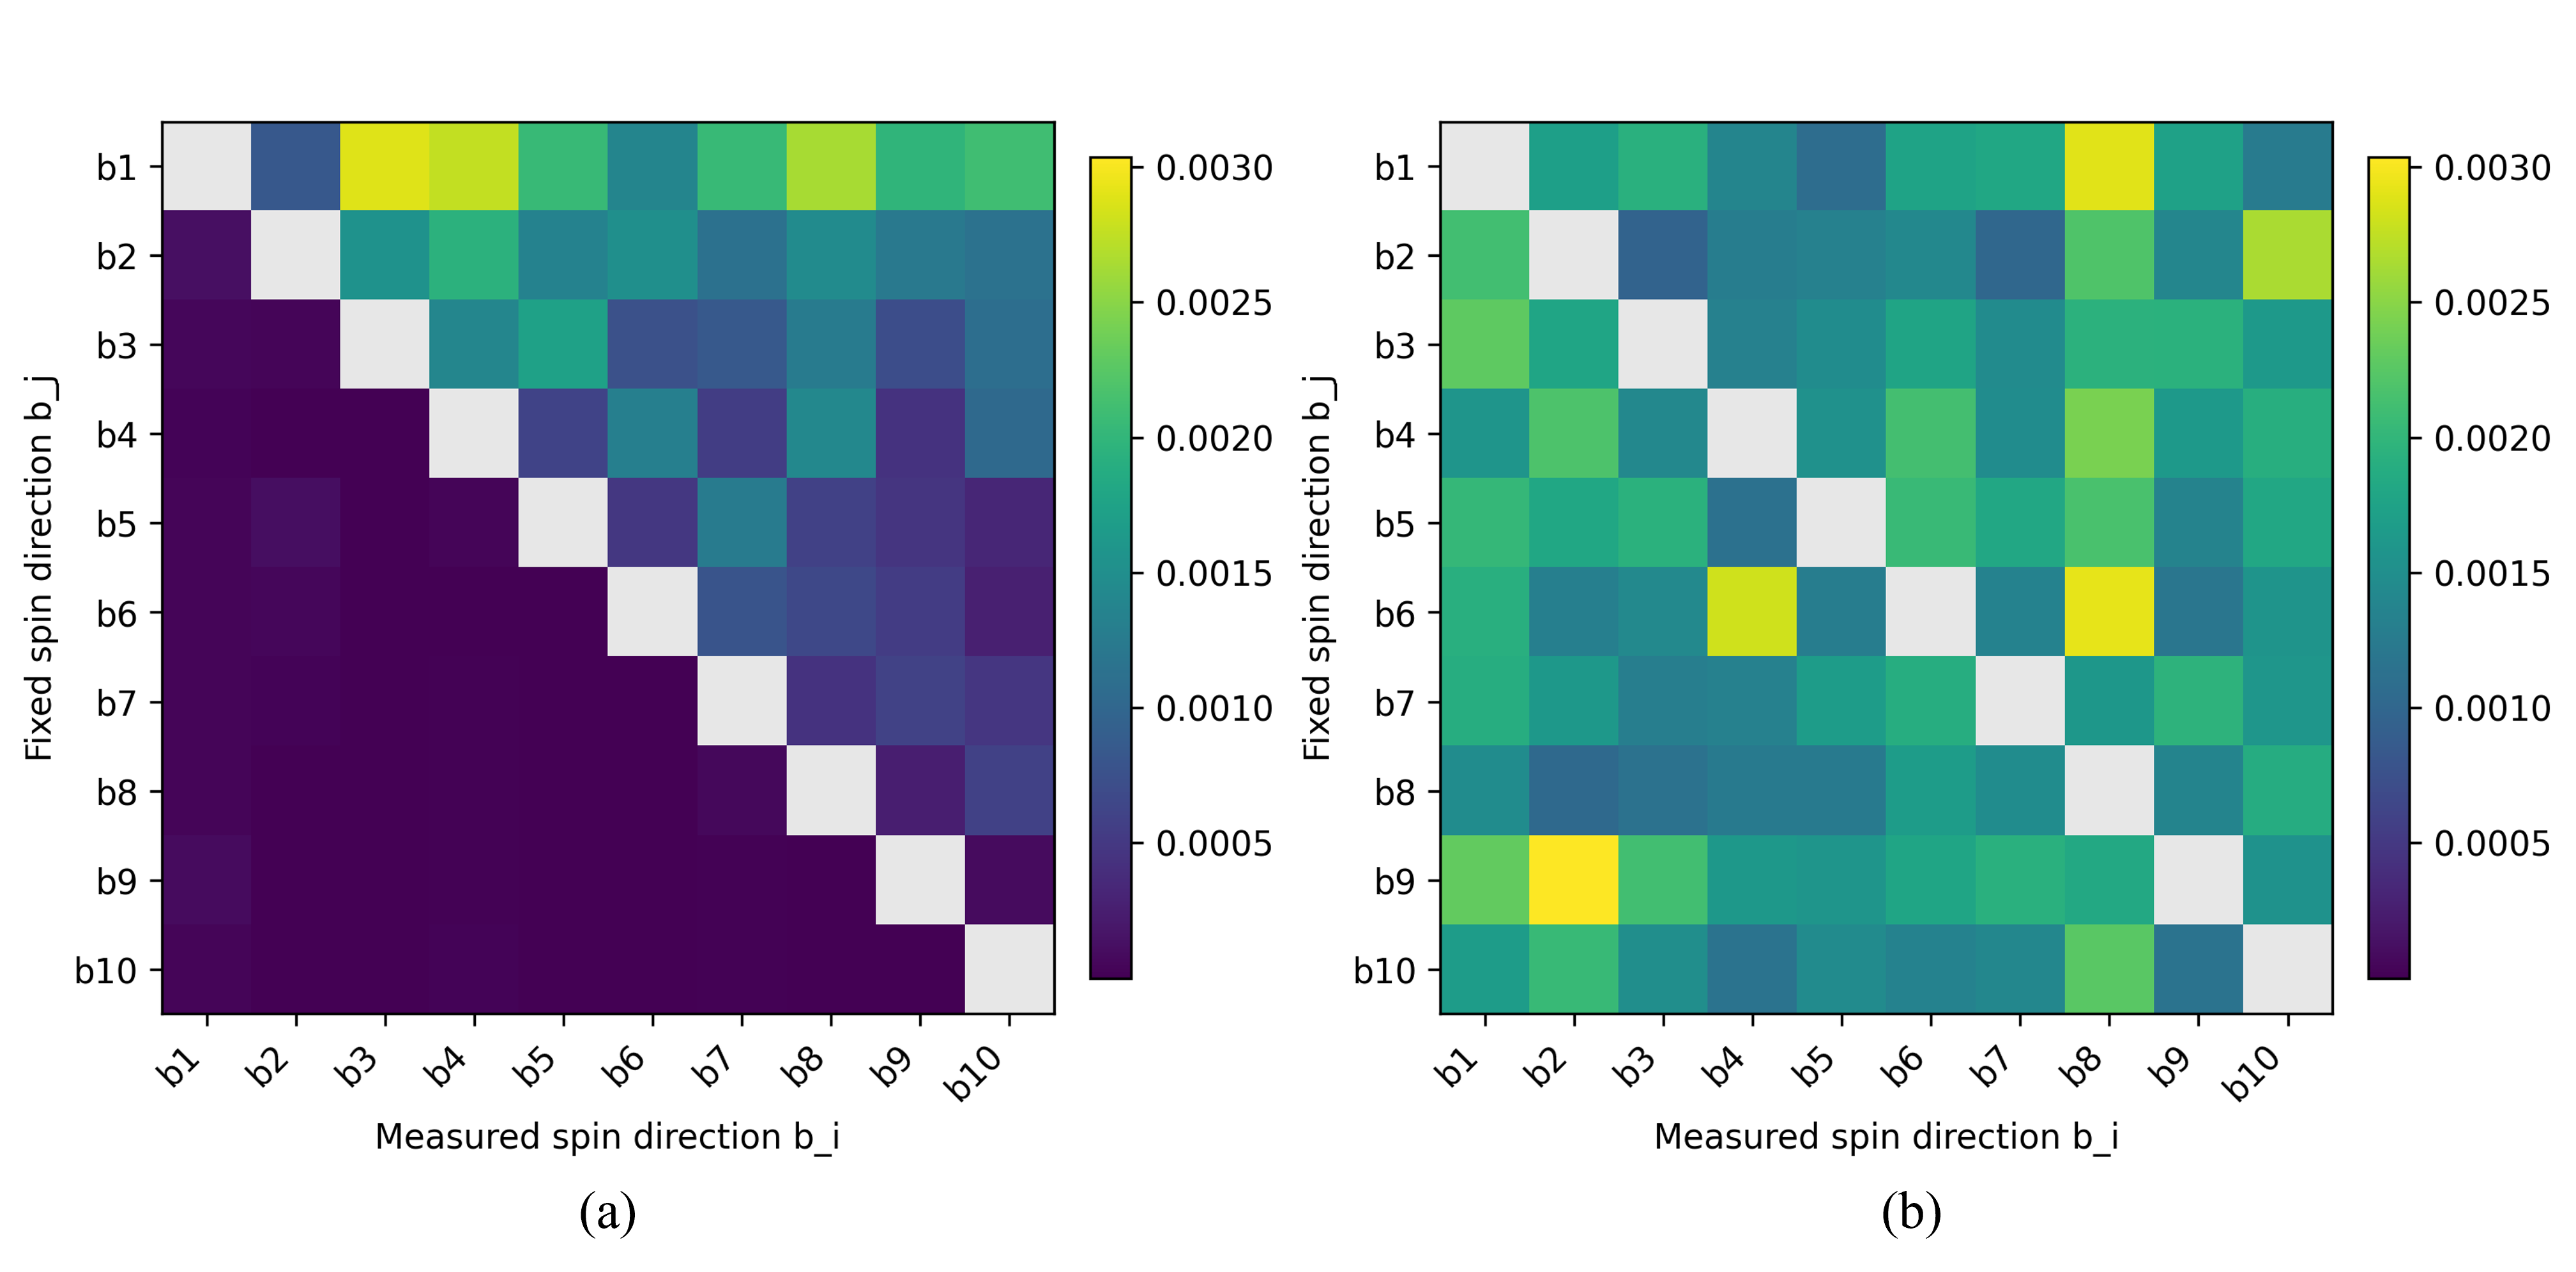
\includegraphics[width=0.98\textwidth]{fig/kl_control_to_experiment_heatmaps2.png}
  \caption{KL divergence of the predicted distributions of the remaining qubits after fixing the measurement outcome of a selected qubit. (a) The result of Diffushadow with causal attention. (b) The result of Diffushadow with full-attention.
  Full attention allows the perturbation to influence both earlier and later sequence positions, whereas causal attention primarily propagates the perturbation to later positions.}
  \label{fig:kl_divergence_attention}    
\end{figure}


\begin{figure}[htbp]
  \centering
  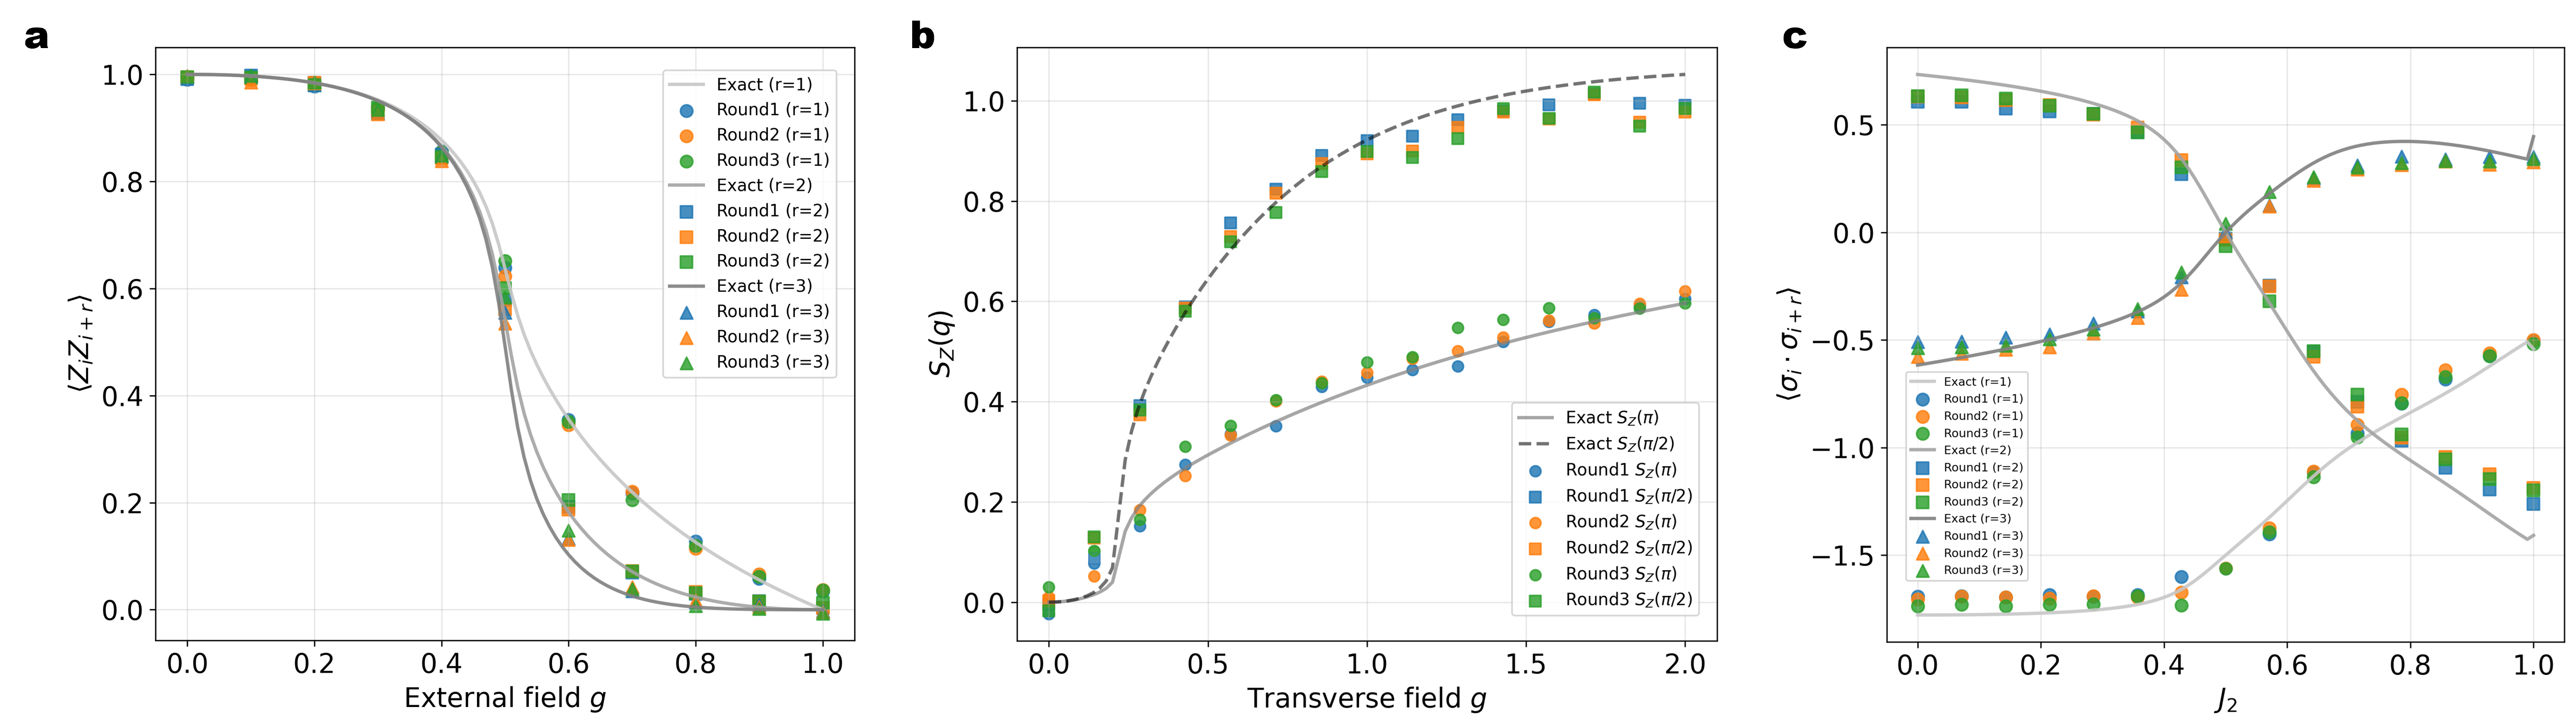
\includegraphics[width=\textwidth]{fig/Figure_stability_all2.0.png}
\caption{\textbf{Consistency of observable estimates across recursive training rounds.}
Observable estimates from Diffushadow models obtained in three recursive training rounds are compared at the common system size $N=24$.
\textbf{a,} Longitudinal spin correlations $\langle Z_i Z_{i+r}\rangle$ at $r=1,2,3$ in the transverse-field Ising (TFI) chain.
\textbf{b,} Longitudinal structure factors $S_Z(\pi)$ and $S_Z(\pi/2)$ in the ANNNI chain.
\textbf{c,} Spin-dot correlations $\langle\boldsymbol{\sigma}_i\cdot\boldsymbol{\sigma}_{i+r}\rangle$ at $r=1,2,3$ in the $J_1$--$J_2$ chain.
Solid or dashed curves denote finite-size exact diagonalization (ED) references, while markers denote estimates from Diffushadow-generated classical-shadow measurements.
The observable estimates remain broadly consistent across the three recursive rounds, indicating limited drift in the tested observables at this system size.}
\label{fig:stability_analysis}
\end{figure}


\begin{figure}[htbp]
  \centering
  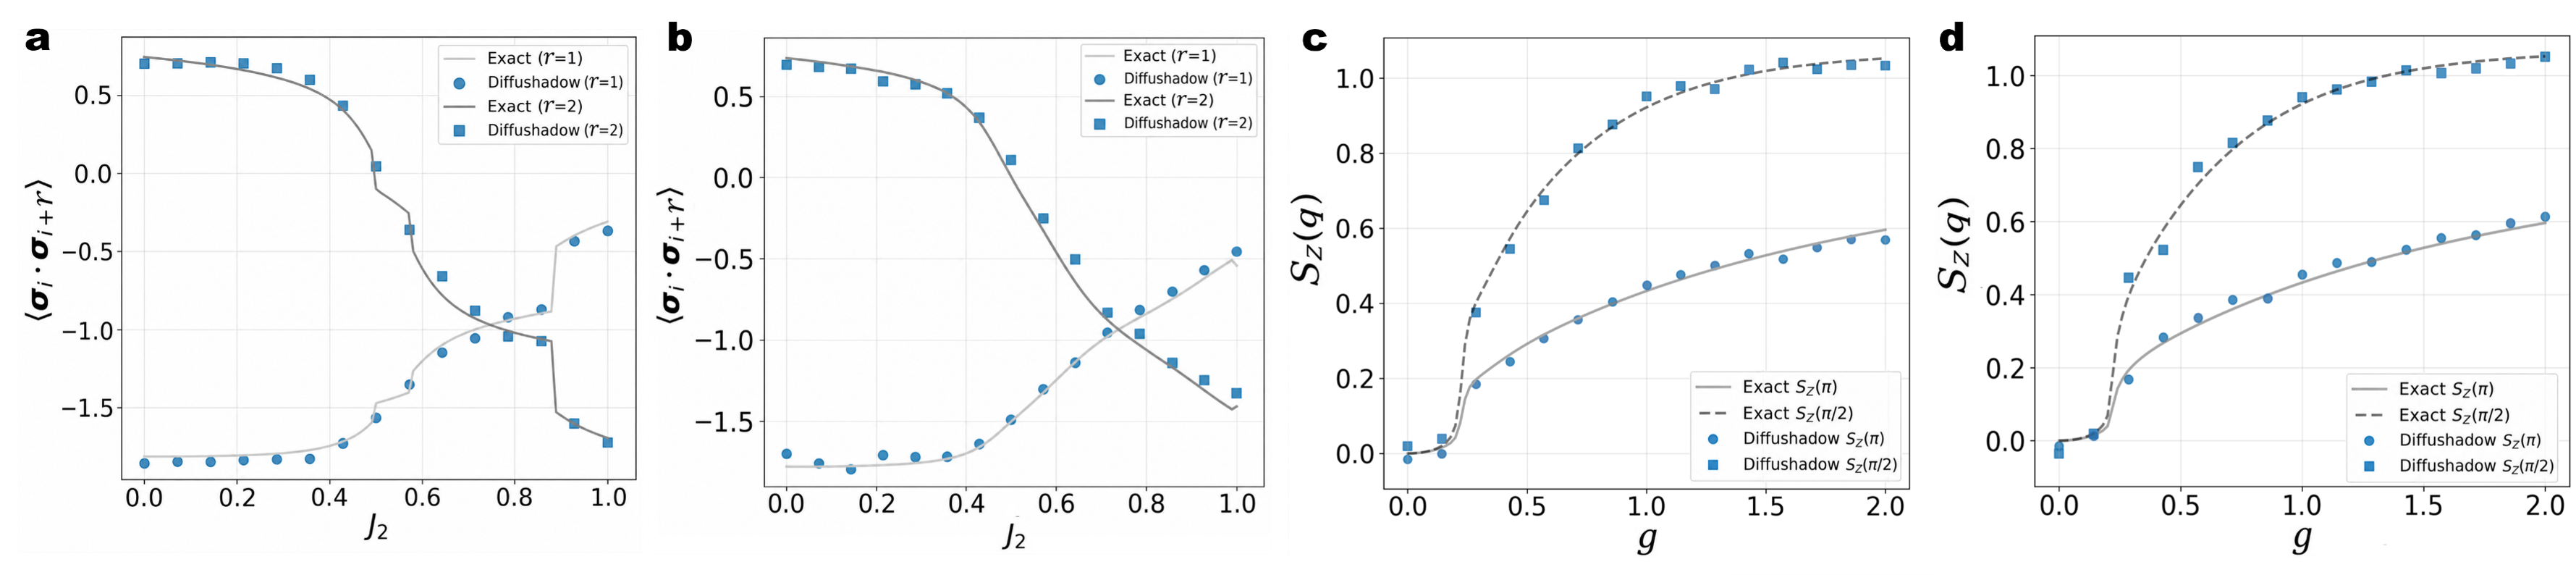
\includegraphics[width=\textwidth]{fig/Figure_J1J2_ANNNI_12_24.png}
    \caption{\textbf{Finite-size observable validation for the $J_1$--$J_2$ and ANNNI chains.}
\textbf{a,b,} Spin-dot correlations
$\langle\boldsymbol{\sigma}_i\cdot\boldsymbol{\sigma}_{i+r}\rangle$
at separations $r=1$ (circles) and $r=2$ (squares) for the
$J_1$--$J_2$ model with $J_1=1$, shown as functions of $J_2$
for $N=12$ (\textbf{a}) and $N=24$ (\textbf{b}).
\textbf{c,d,} Longitudinal structure factors $S_Z(q)$
at $q=\pi$ (circles) and $q=\pi/2$ (squares) for the
ANNNI model at fixed $\kappa=0.4$, shown as functions of
$g$ for $N=12$ (\textbf{c}) and $N=24$ (\textbf{d}).
Blue markers denote estimates from Diffushadow-generated
classical-shadow measurements, and grey lines denote
finite-size exact diagonalization (ED) references.
The size $N=12$ is included in the initial training set,
whereas $N=24$ is absent from it.}
    \label{fig:J1J2_ANNNI_12_24}    
\end{figure}







% \begin{table*}[htbp]
% \centering
% \small
% \caption{
% Calibration of finite-size extrapolation using exact transverse-field
% Ising correlations. Exact finite-size correlations evaluated at the
% same system sizes used in the main analysis are extrapolated using
% linear and quadratic expansions in \(1/N\). The extrapolation error is
% defined as
% \(\Delta_{\mathrm{ext}}
% =
% |C_{\infty}^{\mathrm{fit}}
% -
% C_{\infty}^{\mathrm{exact}}|\).
% The critical-region mean absolute error (MAE) is evaluated over
% \(|g-g_c|\leq0.1\), with \(g_c=0.5\).
% }
% \label{tab:tfi_extrapolation_calibration}
% \begin{tabular}{clcccc}
% \hline
% \(r\) &
% Fit &
% MAE (all \(g\)) &
% MAE (critical region) &
% Maximum error &
% \(g\) at maximum \\
% \hline
% \multirow{2}{*}{1}
% & Linear
% & \(2.965\times10^{-4}\)
% & \(1.390\times10^{-3}\)
% & \(2.193\times10^{-3}\)
% & \(0.5714\) \\
% & Quadratic
% & \(\mathbf{1.556\times10^{-4}}\)
% & \(\mathbf{6.925\times10^{-4}}\)
% & \(\mathbf{1.261\times10^{-3}}\)
% & \(0.5714\) \\
% \hline
% \multirow{2}{*}{10}
% & Linear
% & \(7.284\times10^{-4}\)
% & \(3.635\times10^{-3}\)
% & \(9.372\times10^{-3}\)
% & \(0.5000\) \\
% & Quadratic
% & \(\mathbf{2.402\times10^{-4}}\)
% & \(\mathbf{1.189\times10^{-3}}\)
% & \(\mathbf{2.348\times10^{-3}}\)
% & \(0.5714\) \\
% \hline
% \end{tabular}
% \end{table*}

% \begin{figure}[htbp]
%   \centering
%   \includegraphics[width=0.98\textwidth]{fig/TFI_extrapolation_Calibration.png}
%     \caption{
%     Calibration of finite-size extrapolation in the transverse-field Ising model using exact correlation data. Absolute extrapolation errors,
%     \(\left|C_{\infty}^{\mathrm{fit}}-C_{\infty}^{\mathrm{exact}}\right|\),
%     are shown as functions of the transverse-field parameter \(g\) for
%     (a) the nearest-neighbor correlation \(\langle Z_iZ_{i+1}\rangle\) and
%     (b) the longer-range correlation \(\langle Z_iZ_{i+10}\rangle\).
%     Exact finite-size correlations evaluated at the same system sizes used in the main analysis are extrapolated using either a linear form,
%     \(C_N=C_{\infty}+a/N\), or a quadratic form,
%     \(C_N=C_{\infty}+a/N+b/N^2\).
%     The fitted intercepts are compared with the exact thermodynamic-limit correlations. The extrapolation errors are concentrated near the critical region around \(g_c=0.5\), particularly for the longer-range correlation, while the quadratic fit substantially reduces the maximum error relative to the linear fit.
%     }
%   \label{fig:tfi_extrapolation_calibration}    
% \end{figure}



% \begin{figure}[htbp]
%   \centering
%   \includegraphics[width=0.98\textwidth]{fig/Figure_stability_all.png}
%   \caption{KL divergence of the predicted distributions of the remaining qubits after fixing the measurement outcome of a selected qubit. (a) The result of Diffushadow with causal attention. (b) The result of Diffushadow.
%   Full attention allows the perturbation to influence both earlier and later sequence positions, whereas causal attention primarily propagates the perturbation to later positions.}
%   \label{fig:kl_divergence_attention}    
% \end{figure}

% %%=============================================================%%
% %% Sample for another appendix section			       %%
% %%=============================================================%%

% %% \section{Example of another appendix section}\label{secA2}%
% %% Appendices may be used for helpful, supporting or essential material that would otherwise 
% %% clutter, break up or be distracting to the text. Appendices can consist of sections, figures, 
% %% tables and equations etc.

% \end{appendices}

%%===========================================================================================%%
%% If you are submitting to one of the Nature Portfolio journals, using the eJP submission   %%
%% system, please include the references within the manuscript file itself. You may do this  %%
%% by copying the reference list from your .bbl file, paste it into the main manuscript .tex %%
%% file, and delete the associated \verb+\bibliography+ commands.                            %%
%%===========================================================================================%%



\end{document}
